\chapter{Diffusion-Inspired Masked Fine-Tuning for Knowledge injection in Autoregressive LLMs}
\label{Appendix C}

% \begin{savequote}[75mm]
% This is some random quote to start off the chapter.
% \qauthor{Firstname lastname}
% \end{savequote}

%\chapter{Diffusion-Inspired Masked Fine-Tuning for Knowledge injection in Autoregressive LLMs}

\begin{figure*}[h]
  \centering
  \resizebox{0.7\textwidth}{!}{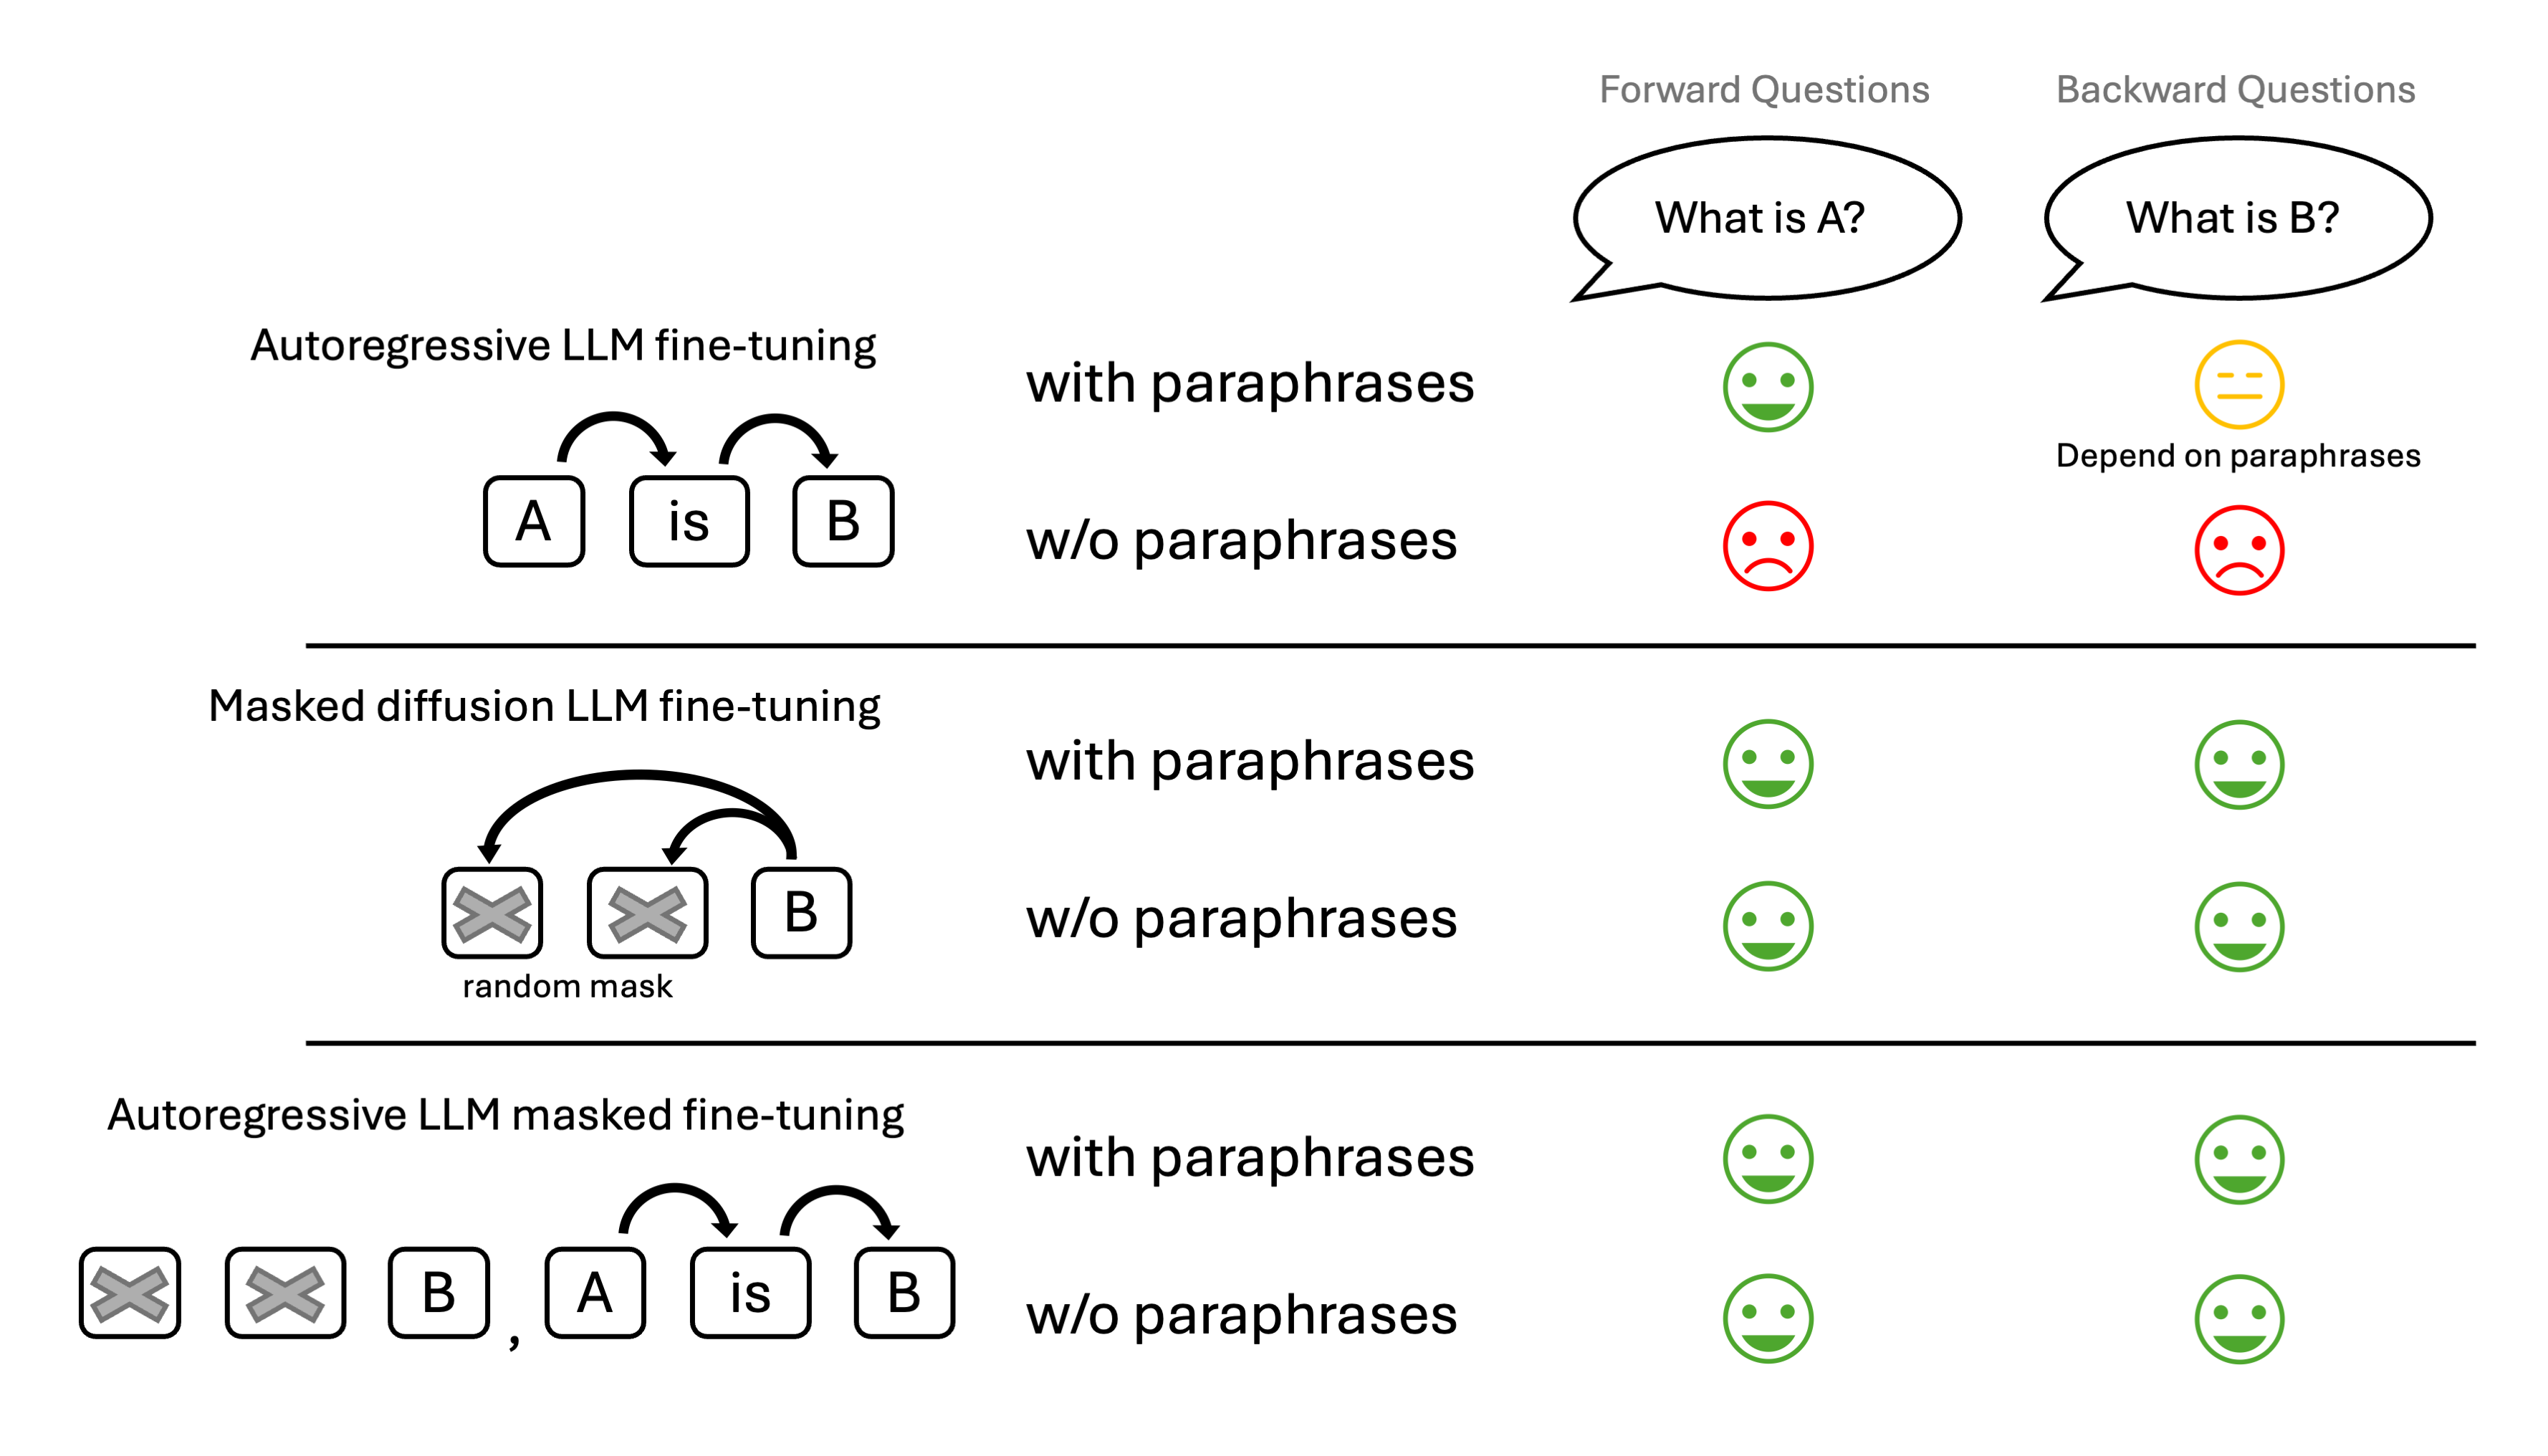
\includegraphics{figures/appendixc_fig01.png}}
  \caption{A schematic summary of the results. First row: autoregressive LLM requires paraphrases to generalize knowledge from the fine-tuning text to QA tasks, and suffers from reversal curse (i.e. fail to answer backward questions). Second row: masked diffusion LLM can easily generalize fine-tuning text to QA tasks in both forward and backward styles. Third row: Inspired by the masked diffusion LLM, we propose a masked fine-tuning paradigm that closes the fine-tuning gap between autoregressive LLMs and masked diffusion LLMs.}
  \label{fig:diagram}
\end{figure*}

\section{Introduction}

Large language models (LLMs) as general assistants are often deployed in settings where facts evolve: news breaks, policies change, and organizations maintain internal knowledge that is continuously updated. A natural idea to keep an LLM up-to-date is to fine-tune the model on newly available documents, in a way similar to pre-training. Yet, a growing body of work shows that fine-tuning on knowledge documents often struggles to translate into reliable downstream question answering (QA) ability, even when the fine-tuning loss decreases \citep{ovadia2023fine, mecklenburg2024injecting, gekhman2024does, soudani2024fine, zhao2025style, lampinen2025generalization}. This gap limits the practicality of weight updating as a long-term memory mechanism in LLMs.

There are two empirical obstacles that make knowledge injection via fine-tuning in autoregressive LLMs (arLLMs) difficult. (1) arLLMs often fail to generalize from raw documents to QA behavior unless the fine-tuning data is expanded with many paraphrases \citep{ovadia2023fine, mecklenburg2024injecting}. This kind of augmentation is expensive and sometimes impractical, as high-quality paraphrases typically require additional LLM calls, careful filtering, and substantial engineering to avoid distribution shift. Such paraphrase dependence indicates that standard fine-tuning may not provide enough training signal from each example. (2) After training on statements whose information is presented in one order (e.g., “A is B”), arLLMs can answer questions aligned with that order but fail catastrophically when asked to invert it (e.g., “B is A”), a behavior known as the reversal curse \citep{berglund2023reversal, zhu24b, lv-etal-2024-analysis, lin2024delving, guo-etal-2024-mitigating, golovneva2024reverse, lu2024rethinking}. The reversal curse is not just “lack of data”, whether augmentation helps depends on whether it re-expresses the same facts in the order demanded by the question.

Recent masked diffusion language models (dLLMs) \citep{ICLR2025_ce1c1ff5, llada, ye2025dream} have revived a bidirectional “denoising” style objective, such as in BERT and T5/Flan-T5 \cite{devlin2019bert, raffel2020exploring}, at LLM scale. Several advantages of dLLMs have been found over arLLMs. During pretraining, dLLMs can reach lower training loss in data-scarce regimes \citep{prabhudesai2025diffusion, ni2025difflm}, suggesting better sample efficiency. After instruction tuning, dLLMs appear less prone to the “reversal curse”; an 8B dLLM has been reported to outperform GPT-4o on a reversal poem completion task \cite{llada}. This motivates our hypothesis about dLLM knowledge injection via fine-tuning:

\textbf{Hypothesis 1}: \textit{Unlike arLLMs, which depend on paraphrase augmentation and exhibit the reversal curse, dLLMs can generalize from fine-tuning on the knowledge text alone to strong QA performance, without additional paraphrased data.}

\begin{sloppypar}
We test this hypothesis in controlled knowledge injection settings. Across datasets, we find that arLLMs strongly depend on paraphrase augmentation for forward QA generalization and still fail on backward QA (an indication of the reversal curse), while dLLMs achieve high accuracy in both directions without paraphrases.
\end{sloppypar}

Since dLLMs' training repeatedly asks the model to reconstruct missing tokens given a partially observed context, this gives the model many distinct conditioning patterns for the same underlying sequence, which can be viewed as implicit augmentation of token order and context availability. This motivates our second hypothesis:

\textbf{Hypothesis 2}: \textit{The knowledge-injection advantage of dLLMs is mainly due to the demasking training objective, rather than diffusion-style decoding or architectural differences. Therefore, adapting a demasking-style fine-tuning objective to decoder-only arLLMs should substantially improve knowledge injection from raw text and largely close the performance gap to dLLMs.}

To test this hypothesis and attempt to transfer dLLM's advantages to arLLM fine-tuning, we propose masked fine-tuning for arLLMs, a simple paradigm that reframes each knowledge document as a reconstruction task. During fine-tuning, we create a masked version of the document, prompt the model to recover the masked passage, and supervise the model on the original unmasked text as the target. By sampling different masks across steps, a single document yields many conditioning patterns, providing bidirectional learning signals while preserving the model’s decoder-only architecture and standard autoregressive training. Empirically, this masked fine-tuning objective substantially improves knowledge injection: it reduces reliance on paraphrase augmentation for forward QA and mitigates the reversal curse for backward QA, largely closing the gap to dLLMs. To probe whether the benefit is specific to factual knowledge injection or also good for procedural knowledge learning, we adapt the demasking formulation to math SFT by masking parts of the target solution and training the model to reconstruct them. Across two math datasets and two arLLMs, masked SFT improves over standard SFT, suggesting a broader applicability of the demasking objective.


\section{Background}

\subsection{Knowledge injection and paraphrase dependence}

Empirically, LLMs can appear to store facts yet fail to extract them under novel question wordings unless the training samples cover a variety of ways that the same fact can be presented. In a synthetic setting, \citet{zhu24a} found that reliable knowledge extraction correlates strongly with paraphrase augmentation during training, and that post-hoc instruction tuning cannot fully recover extractability if the pretraining signal lacks such variation. In a more realistic setting involving Wikipedia knowledge injection into instruction-tuned LLMs, \citet{ovadia2023fine} and \citet{mecklenburg2024injecting} found that QA capability scales with the number of paraphrases used in training but saturates quickly at around 10 paraphrases per sample and still lags behind retrieval-based methods such as RAG. \citet{ovadia2025knowledge} showed that a multi-stage data augmentation pipeline—first breaking articles down into individual concepts and facts and then paraphrasing—can further improve QA accuracy, but such methods are extremely expensive and rely on a strong LLM to prepare the data.

\subsection{Reversal curse}

The reversal curse describes a failure mode in LLM training in which, after learning statements of the form “A is B,” a model does not generalize to the inverse form “B is A.” The reversal curse has been observed across training phases and model families \citep{berglund2023reversal, zhu24b, lv-etal-2024-analysis, lin2024delving, guo-etal-2024-mitigating, golovneva2024reverse, lu2024rethinking}. Even commercial models such as GPT-4 and GPT-4o show signs of the reversal curse \citep{berglund2023reversal, llada}. The reversal curse has been theoretically attributed to an inherent limitation of the autoregressive training objective \citep{zhu2024towards, kitouni2024factorization} (see Appendix \ref{app:reversal} for further discussion). Common approaches to mitigating the reversal curse in autoregressive models include: (i) augmenting the training set with paraphrases \citep{lu2024rethinking}, which requires substantial computation to construct; (ii) augmenting the training set with reordered sequences \citep{guo-etal-2024-mitigating, golovneva2024reverse}, which often violates natural-language grammar and degrades overall language modeling performance; and (iii) replacing causal attention with bidirectional attention \citep{lv-etal-2024-analysis}, which struggles to retrieve information over long contexts (e.g., a person’s description). In contrast, our proposed masked fine-tuning paradigm (Section \ref{section:6}) for arLLMs addresses the reversal curse without constructing paraphrase augmentations or altering the autoregressive objective; it only requires rewriting the training sample into a demasking task.

\subsection{Demasking objective in language models}


Recently, dLLMs have emerged as a strong competitor to arLLMs \citep{sahoo2024simple, llada, ye2025dream}. Compared to autoregressive models, dLLMs use bidirectional attention (non-causal) to generate text by iteratively demasking tokens via a reversed discrete diffusion process. The training objective is to minimize the mask reconstruction loss \cite{llada}:

\begin{equation}
\mathcal{L}(\theta) = -\mathbb{E}_{t,\boldsymbol{x}_0,\boldsymbol{x}_t}\left[\frac{1}{t}\sum_{\ell=1}^{L}\mathbb{I}[\boldsymbol{x}_t^{\ell} \in \text{M}]\log p_\theta(\boldsymbol{x}_0^{\ell}|\boldsymbol{x}_t)\right],
\label{eq:1}
\end{equation}

$\boldsymbol{x_0}$ is an original sequence of length $L$ sampled from the training data. The masking process is governed by the mask ratio $t$, which is sampled uniformly, resulting in the corrupted sequence $\boldsymbol{x_t}$. The set $\mathbf{M}$ denotes the indices of the tokens that were masked by the forward process at ratio $t$. The $\ell$-th token is considered for the loss only if it was masked. Such a loss objective has been shown to be the negative evidence lower bound (ELBO) on the data likelihood \citep{shi2024simplified}.

Recent studies report dLLMs are more sample-efficient than arLLMs. When the training data is scarce, dLLMs keep improving with repeated use of the data and surpass arLLMs on validation loss, while arLLMs saturate the validation loss or increase it due to overfitting \citep{prabhudesai2025diffusion, ni2025difflm}. \citet{prabhudesai2025diffusion} further shows that the lower validation loss in dLLMs can generalize to downstream tasks like ARC-Easy, and attributes its data efficiency to random masks as implicit data augmentation. However, whether these advantages persist in new knowledge acquisition during post-training—where the model needs to learn generalizable knowledge through small fine-tuning sets—remains unclear. 

\newtcbox{\grayhl}{on line, tcbox raise base,
  colback=pink!30, colframe=pink!30,
  boxrule=0pt, arc=0pt,
  boxsep=0pt, left=1pt, right=1pt, top=0pt, bottom=0pt,
  before upper=\strut % match the line’s height/depth for the current font size
}

\newtcbox{\pinkhl}{on line, tcbox raise base,
  colback=cyan!20!green!10, colframe=cyan!20!green!10,
  boxrule=0pt, arc=0pt,
  boxsep=0pt, left=1pt, right=1pt, top=0pt, bottom=0pt,
  before upper=\strut % match the line’s height/depth for the current font size
}


\begin{table*}[t]
      \caption{Fine-tuning performance of the dLLM and arLLMs across all three datasets. Model names are shortened for presentation (see section \ref{sec:setup} for full model names). ``Masked'' denotes the masked fine-tuning paradigm. ``Reverse training'' denotes the entity-level reverse-training paradigm proposed in \cite{golovneva2024reverse}, which we use as a baseline control. For the Wiki dataset, we use the same-order paraphrase set. Pink indicates clear failure (accuracy below 50\%); turquoise indicates clear success (accuracy above 90\%).}
    \label{tab:3}
  \begin{center}
    % \begin{scriptsize}
    {\fontsize{8.5}{10}\selectfont
      % \begin{sc}
        \setlength{\tabcolsep}{4pt}
        \resizebox{\textwidth}{!}{\begin{tabular}{lcccccccc}
        \toprule
        & \multicolumn{4}{c}{NameDescription} & \multicolumn{2}{c}{Biography} & \multicolumn{2}{c}{Wiki} \\
        \cmidrule(lr){2-5}\cmidrule(lr){6-7}\cmidrule(lr){8-9}
         & N2D-fwd & N2D-bwd & D2N-fwd & D2N-bwd & Fwd & Bwd & Fwd & Bwd \\
        \midrule
        
        Llada before fine-tuning        & \grayhl{0.030} & \grayhl{0.000} & \grayhl{0.028} & \grayhl{0.000} & \grayhl{0.030} & \grayhl{0.000} & \grayhl{0.210} & \grayhl{0.156} \\
        Llada w/o paraphrases      & 0.873 & \pinkhl{0.913} & 0.864 & 0.790 & 0.892 & 0.696 & \pinkhl{0.908} & 0.778 \\
        Llada w paraphrases        & \pinkhl{0.967} & \pinkhl{0.994} & \pinkhl{0.994} & \pinkhl{0.973} & \pinkhl{0.991} & 0.857 & \pinkhl{0.900} & 0.785 \\
        \midrule
        Llama 8B before fine-tuning     & \grayhl{0.072} & \grayhl{0.000} & \grayhl{0.054} & \grayhl{0.000}  & \grayhl{0.001} & \grayhl{0.000} & \grayhl{0.164} & \grayhl{0.127} \\
        Llama 8B reverse training       & 0.637 & \grayhl{0.125} & \grayhl{0.113} & \grayhl{0.088} & \grayhl{0.180} & \grayhl{0.011} & 0.609 & \grayhl{0.425} \\
        Llama 8B w/o paraphrases        & \grayhl{0.374} & \grayhl{0.000} & \grayhl{0.017} & \grayhl{0.027} & \grayhl{0.121} & \grayhl{0.002} & \grayhl{0.377} & \grayhl{0.282} \\
        Llama 8B w paraphrases          & \pinkhl{0.910} & \grayhl{0.004} & \pinkhl{0.925} & \grayhl{0.071} & \pinkhl{0.962} & \grayhl{0.001} & 0.685 & \grayhl{0.396} \\
        Masked Llama 8B w/o paraphrases (ours) & 0.658 & \pinkhl{0.949} & \pinkhl{0.992} & \pinkhl{0.923} & \pinkhl{0.971} & 0.598 & \pinkhl{0.980} & \pinkhl{0.930} \\
        Masked Llama 8B w paraphrases (ours)  & \pinkhl{0.969} & \pinkhl{0.996} & \pinkhl{0.928} & 0.832 & \pinkhl{0.965} & 0.816 & \pinkhl{0.905} & 0.794 \\
        \midrule
        Llama 3B before fine-tuning     & \grayhl{0.078} & \grayhl{0.067} & \grayhl{0.000} & \grayhl{0.000} & \grayhl{0.001} & \grayhl{0.001} & \grayhl{0.106} & \grayhl{0.159} \\
        Llama 3B reverse training       & \grayhl{0.391} & \grayhl{0.079} & \grayhl{0.042} & \grayhl{0.025} & \grayhl{0.216} &  \grayhl{0.003} & \grayhl{0.384} & \grayhl{0.285} \\
        Llama 3B w/o paraphrases        & \grayhl{0.230} & \grayhl{0.078} & \grayhl{0.017} & \grayhl{0.000} & \grayhl{0.032} & \grayhl{0.000} & \grayhl{0.292} & \grayhl{0.229} \\
        Llama 3B w paraphrases          & \pinkhl{0.951} & \grayhl{0.040} & \pinkhl{0.967} & \grayhl{0.025} & \pinkhl{0.988} & \grayhl{0.001} & 0.622 & \grayhl{0.334} \\
        Masked Llama 3B w/o paraphrases (ours) & 0.887 & \pinkhl{0.932} & \pinkhl{0.992} & \pinkhl{0.933} & \pinkhl{0.967} & 0.738 & \pinkhl{0.970} & \pinkhl{0.908} \\
        Masked Llama 3B w paraphrases (ours)  & \pinkhl{0.982} & \pinkhl{0.928} & \pinkhl{1.000} & \pinkhl{0.992} & \pinkhl{0.964} & 0.809 & 0.855 & 0.810 \\
        \midrule
        Qwen 7B before fine-tuning     & \grayhl{0.039} & \grayhl{0.030} & \grayhl{0.000} & \grayhl{0.000} & \grayhl{0.018} & \grayhl{0.000} & \grayhl{0.205} & \grayhl{0.231} \\
        Qwen 7B reverse training       & \pinkhl{0.902} & \grayhl{0.092} & \grayhl{0.450} & \grayhl{0.350}  & 0.540  & \grayhl{0.026} & 0.678 & \grayhl{0.481} \\
        Qwen 7B w/o paraphrases        & \pinkhl{0.966} & \grayhl{0.043} & \grayhl{0.367} & \grayhl{0.000} & \grayhl{0.357} & \grayhl{0.003} & 0.676 & \grayhl{0.371} \\
        Qwen 7B w paraphrases          & \pinkhl{0.987} & \grayhl{0.063} & \pinkhl{0.954} & \grayhl{0.000} & \pinkhl{0.956} & \grayhl{0.003} & 0.712 & \grayhl{0.414} \\
        Masked Qwen 7B w/o paraphrases (ours) & 0.870 & 0.897 & \pinkhl{0.967} & \pinkhl{0.929} & \pinkhl{0.984} & 0.754 & \pinkhl{0.934} & 0.896 \\
        Masked Qwen 7B w paraphrases (ours)  & \pinkhl{0.957} & 0.810 & \pinkhl{0.933} & \pinkhl{1.000} & \pinkhl{0.960} & 0.828 & 0.867 & 0.821 \\
        \midrule
        Qwen 4B before fine-tuning     & \grayhl{0.026} & \grayhl{0.032} & \grayhl{0.000} & \grayhl{0.000} & \grayhl{0.058} & \grayhl{0.001} & \grayhl{0.237} & \grayhl{0.243} \\
        Qwen 4B reverse training       & \grayhl{0.259} & \grayhl{0.083} & \grayhl{0.008} & \grayhl{0.008} & \grayhl{0.140} & \grayhl{0.008} & \grayhl{0.470} & \grayhl{0.437} \\
        Qwen 4B w/o paraphrases        & \grayhl{0.137} & \grayhl{0.081} & \grayhl{0.000} & \grayhl{0.000} & \grayhl{0.103} & \grayhl{0.001} & 0.509 & \grayhl{0.353} \\
        Qwen 4B w paraphrases          & \pinkhl{0.962} & \grayhl{0.038} & \pinkhl{0.975} & \grayhl{0.000} & \pinkhl{0.994} & \grayhl{0.003} & 0.675 & \grayhl{0.418} \\
        Masked Qwen 4B w/o paraphrases (ours) & \pinkhl{0.928} & \pinkhl{0.902} & \pinkhl{0.950} & \pinkhl{0.967} & \pinkhl{0.944} & 0.623 & \pinkhl{0.907} & 0.870 \\
        Masked Qwen 4B w paraphrases (ours)  & \pinkhl{0.975} & 0.816 & \pinkhl{1.000} & \pinkhl{0.975} & \pinkhl{0.967} & 0.806 & 0.847 & 0.822 \\
        \bottomrule
        \end{tabular}}
      % \end{sc}
    % \end{scriptsize}
    }
    \vskip 0.1in

  \end{center}
  \vskip -0.1in
\end{table*}


\section{Datasets and experimental setups}

\label{sec:setup}

We focus on assessing LLMs' ability to learn new knowledge through fine-tuning. More specifically, LLMs are fine-tuned on a set of documents that contain knowledge unknown to the base LLM, and evaluated by open-ended QA tasks. The correctness of an answer is evaluated by the ROUGE-1 score \citep{lin2024delving, jiang2025anyedit} between the generated answer and the ground truth answer, which is reported as ``accuracy'' for brevity. It measures the proportion of the words in the ground truth answer that appear in the generated answer. To better demonstrate the generation quality, we also show examples of model responses in all the experiments in \ref{app:example}.    

We use three representative datasets. Two are existing synthetic datasets from prior reversal-curse studies, each accompanied by a paraphrase set for data augmentation; the third is constructed from Wikipedia articles about recent events. Prior work on the reversal curse has rarely used realistic datasets. We include the Wikipedia dataset to probe the reversal curse in a setting that better reflects real-world knowledge acquisition, where new events continually occur and models must absorb and retain them. See examples of each dataset in Appendix \ref{app:dataset}.

The \textbf{\textit{NameDescription}} \citep{berglund2023reversal} contains 60 statements of different fictitious individuals, 30 each of the form ``[name] is [description]'' (N2D) and ``[description] is [name]'' (D2N). \cite{lin2024delving} extended the dataset with an open-ended QA testing set. For each type of statement, the QA set contains two types of questions: ``What is the name related to a given description'' and ``What is the description of a given name''. Depending on whether the question is aligned with the original statement, each question is classified as ``forward'' or ``backward'' question (e.g. N2D statement with ``What is the description of a given name'' type of question is a forward question). The dataset also contains a paraphrase set, in which each statement is rewritten into 30 different versions, but the order of [name] and [description] in the paraphrases is always preserved as in the original statement (either N2D or D2N).

The \textbf{\textit{Biography}} dataset is proposed in \cite{zhu24a,zhu24b}. Since the original dataset is not publicly available, we used a subset of 100 samples from a replication \citep{zheng2025spurious}. Each sample is a 6-sentence paragraph about a fictitious individual, detailing their birth city, birthday, college, and job information. Note that the name only appears in the first sentence and is replaced with a pronoun in the following sentences; thus, questions about the name are considered backward questions. Each sample also includes a paraphrase set of 5 paraphrases; the paraphrases do not change the order of the sentences but only alter the wording while preserving the information. The testing QA set has both forward (i.e., asking for an attribute given the name) and backward styles (i.e., asking for the name given 3 attributes from the person) questions.

The \textbf{\textit{Wiki}} dataset contains 94 Wikipedia articles, constructed according to the protocol described in \cite{pan2025memorization}. We crawl the Wikipedia pages under the category ``2025 by month'', and then further filter out the pages that were created before the year 2025. This procedure ensures that these real-world events are recent enough that both dLLM and arLLM models have minimal knowledge about them, which is justified by the models' accuracy before fine-tuning (Table \ref{tab:3}). For each wiki article, we use GPT-o3-mini to generate QA pairs in both forward and backward styles. By prompting GPT-o3-mini, we construct two different paraphrase sets: one that retains the information in place while only changing the wording (same-order paraphrases); the other also changes the order of information in the article (permute-order paraphrases). 10 paraphrases of each type are generated for every wiki article. All LLM generated QAs or paraphrases are cross-checked by human and invalid entries are filtered out and replaced. More details on constructing the datasets are provided in Appendix \ref{app:dataset}.

We chose the arLLMs Llama-3.1-8B-Instruct, Llama-3.2-3B-Instruct \citep{dubey2024llama}, Qwen2.5-7B-Instruct, Qwen3-4B-Instruct-2507 \cite{yang2025qwen3} and dLLM LLaDA-8B-Instruct \citep{llada} to conduct the experiments. LLaDA-8B-Instruct is directly comparable to Llama-3.1-8B-Instruct as they have similar parameter size and comparable general capability benchmarks. Fine-tuning and evaluation configurations are provided in Appendix \ref{app:fine-tuning}.

\section{Results}

\subsection{Failures of arLLM knowledge injection}


We first show that knowledge injection by fine-tuning in arLLMs heavily relies on paraphrases. This is known in previous studies \citep{berglund2023reversal, zhu24b, lin2024delving, guo-etal-2024-mitigating, golovneva2024reverse}. We demonstrate this observation on three datasets to set baselines for comparison with dLLM and our novel paradigm in the following sections. %including our originally constructed Wiki dataset that represents a more realistic learning setting than previously used synthetic datasets.

We fine-tune arLLMs on samples from each dataset using the pre-training format (i.e., without a chat template; using a chat template yields similar results, Figure \ref{fig:fix_t} t=1.). Without paraphrases, backward accuracy on the NameDescription and Biography datasets is close to 0, while the forward accuracy of NameDescription N2D and Biography does not completely fail but is still poor (Table \ref{tab:3}). Adding same-order paraphrases drastically raises forward accuracy close to 1, while backward accuracy remains close to 0. Paraphrases do not help backward accuracy in NameDescription and Biography datasets because the construction of these datasets does not change the semantic order of the sentences.
The trend is similar in the Wiki dataset (Table \ref{tab:3} and \ref{tab:2}). While the same-order paraphrases significantly increase forward accuracy, they only mildly increase backward accuracy. Using permute-order paraphrases increases both forward and backward accuracy, and the gap between them is smaller. Note that, due to the naturalness of this dataset, pre-fine-tuning accuracies are not as close to zero as in the other datasets (Table \ref{tab:3} and \ref{tab:2}); nonetheless, they are sufficiently low to demonstrate the effectiveness of fine-tuning.

\begin{table}[h]
  \caption{Fine-tuning performance of arLLM on the Wiki dataset. Pink indicates clear failure (accuracy below 50\%).}
\label{tab:2}
  \begin{center}
    % \begin{footnotesize}
    {\fontsize{8}{9}\selectfont
      % \begin{sc}
        \setlength{\tabcolsep}{4pt}
        \begin{tabular}{lcc}
          \toprule
          & \multicolumn{2}{c}{Wiki} \\
          \cmidrule(lr){2-3}
          Model / Setting & Fwd & Bwd \\
          \midrule
          Llama 8B before fine-tuning          & \grayhl{0.164} & \grayhl{0.127} \\
          Llama 8B w/o paraphrases             & \grayhl{0.377} & \grayhl{0.282} \\
          Llama 8B w same-order paraphrases    & 0.685          & \grayhl{0.396} \\
          Llama 8B w permute-order paraphrases & 0.721          & 0.628 \\
          \midrule
          Llama 3B before fine-tuning          & \grayhl{0.106} & \grayhl{0.159} \\
          Llama 3B w/o paraphrases             & \grayhl{0.292} & \grayhl{0.229} \\
          Llama 3B w same-order paraphrases    & 0.622          & \grayhl{0.334} \\
          Llama 3B w permute-order paraphrases & 0.667          & 0.550 \\
          \midrule
          Qwen 7B before fine-tuning           & \grayhl{0.205} & \grayhl{0.231} \\
          Qwen 7B w/o paraphrases              & 0.676          & \grayhl{0.371} \\
          Qwen 7B w same-order paraphrases     & 0.712          & \grayhl{0.414} \\
          Qwen 7B w permute-order paraphrases  & 0.761          & 0.621 \\
          \midrule
          Qwen 4B before fine-tuning           & \grayhl{0.237} & \grayhl{0.243} \\
          Qwen 4B w/o paraphrases              & 0.509          & \grayhl{0.353} \\
          Qwen 4B w same-order paraphrases     & 0.675          & \grayhl{0.418} \\
          Qwen 4B w permute-order paraphrases  & 0.693          & 0.639 \\
          \bottomrule
        \end{tabular}
      % \end{sc}
    % \end{footnotesize}
    }
    \vskip 0in

  \end{center}
  \vskip -0in
\end{table}

These results suggest that, in arLLM fine-tuning, paraphrases significantly improve QA accuracy, but help backward questions only when the paraphrases change the information order in the original text to be more aligned with the backward style. Note that the accuracy difference between fine-tuning with paraphrases and without paraphrases is not due to different training steps; in both cases, we train the models with a sufficiently large number of epochs; the reported accuracy is taken from the best checkpoint during the training (Figure \ref{fig:main} and Appendix Figure \ref{fig:total_acc}).

\begin{figure*}[t]
  \centering
  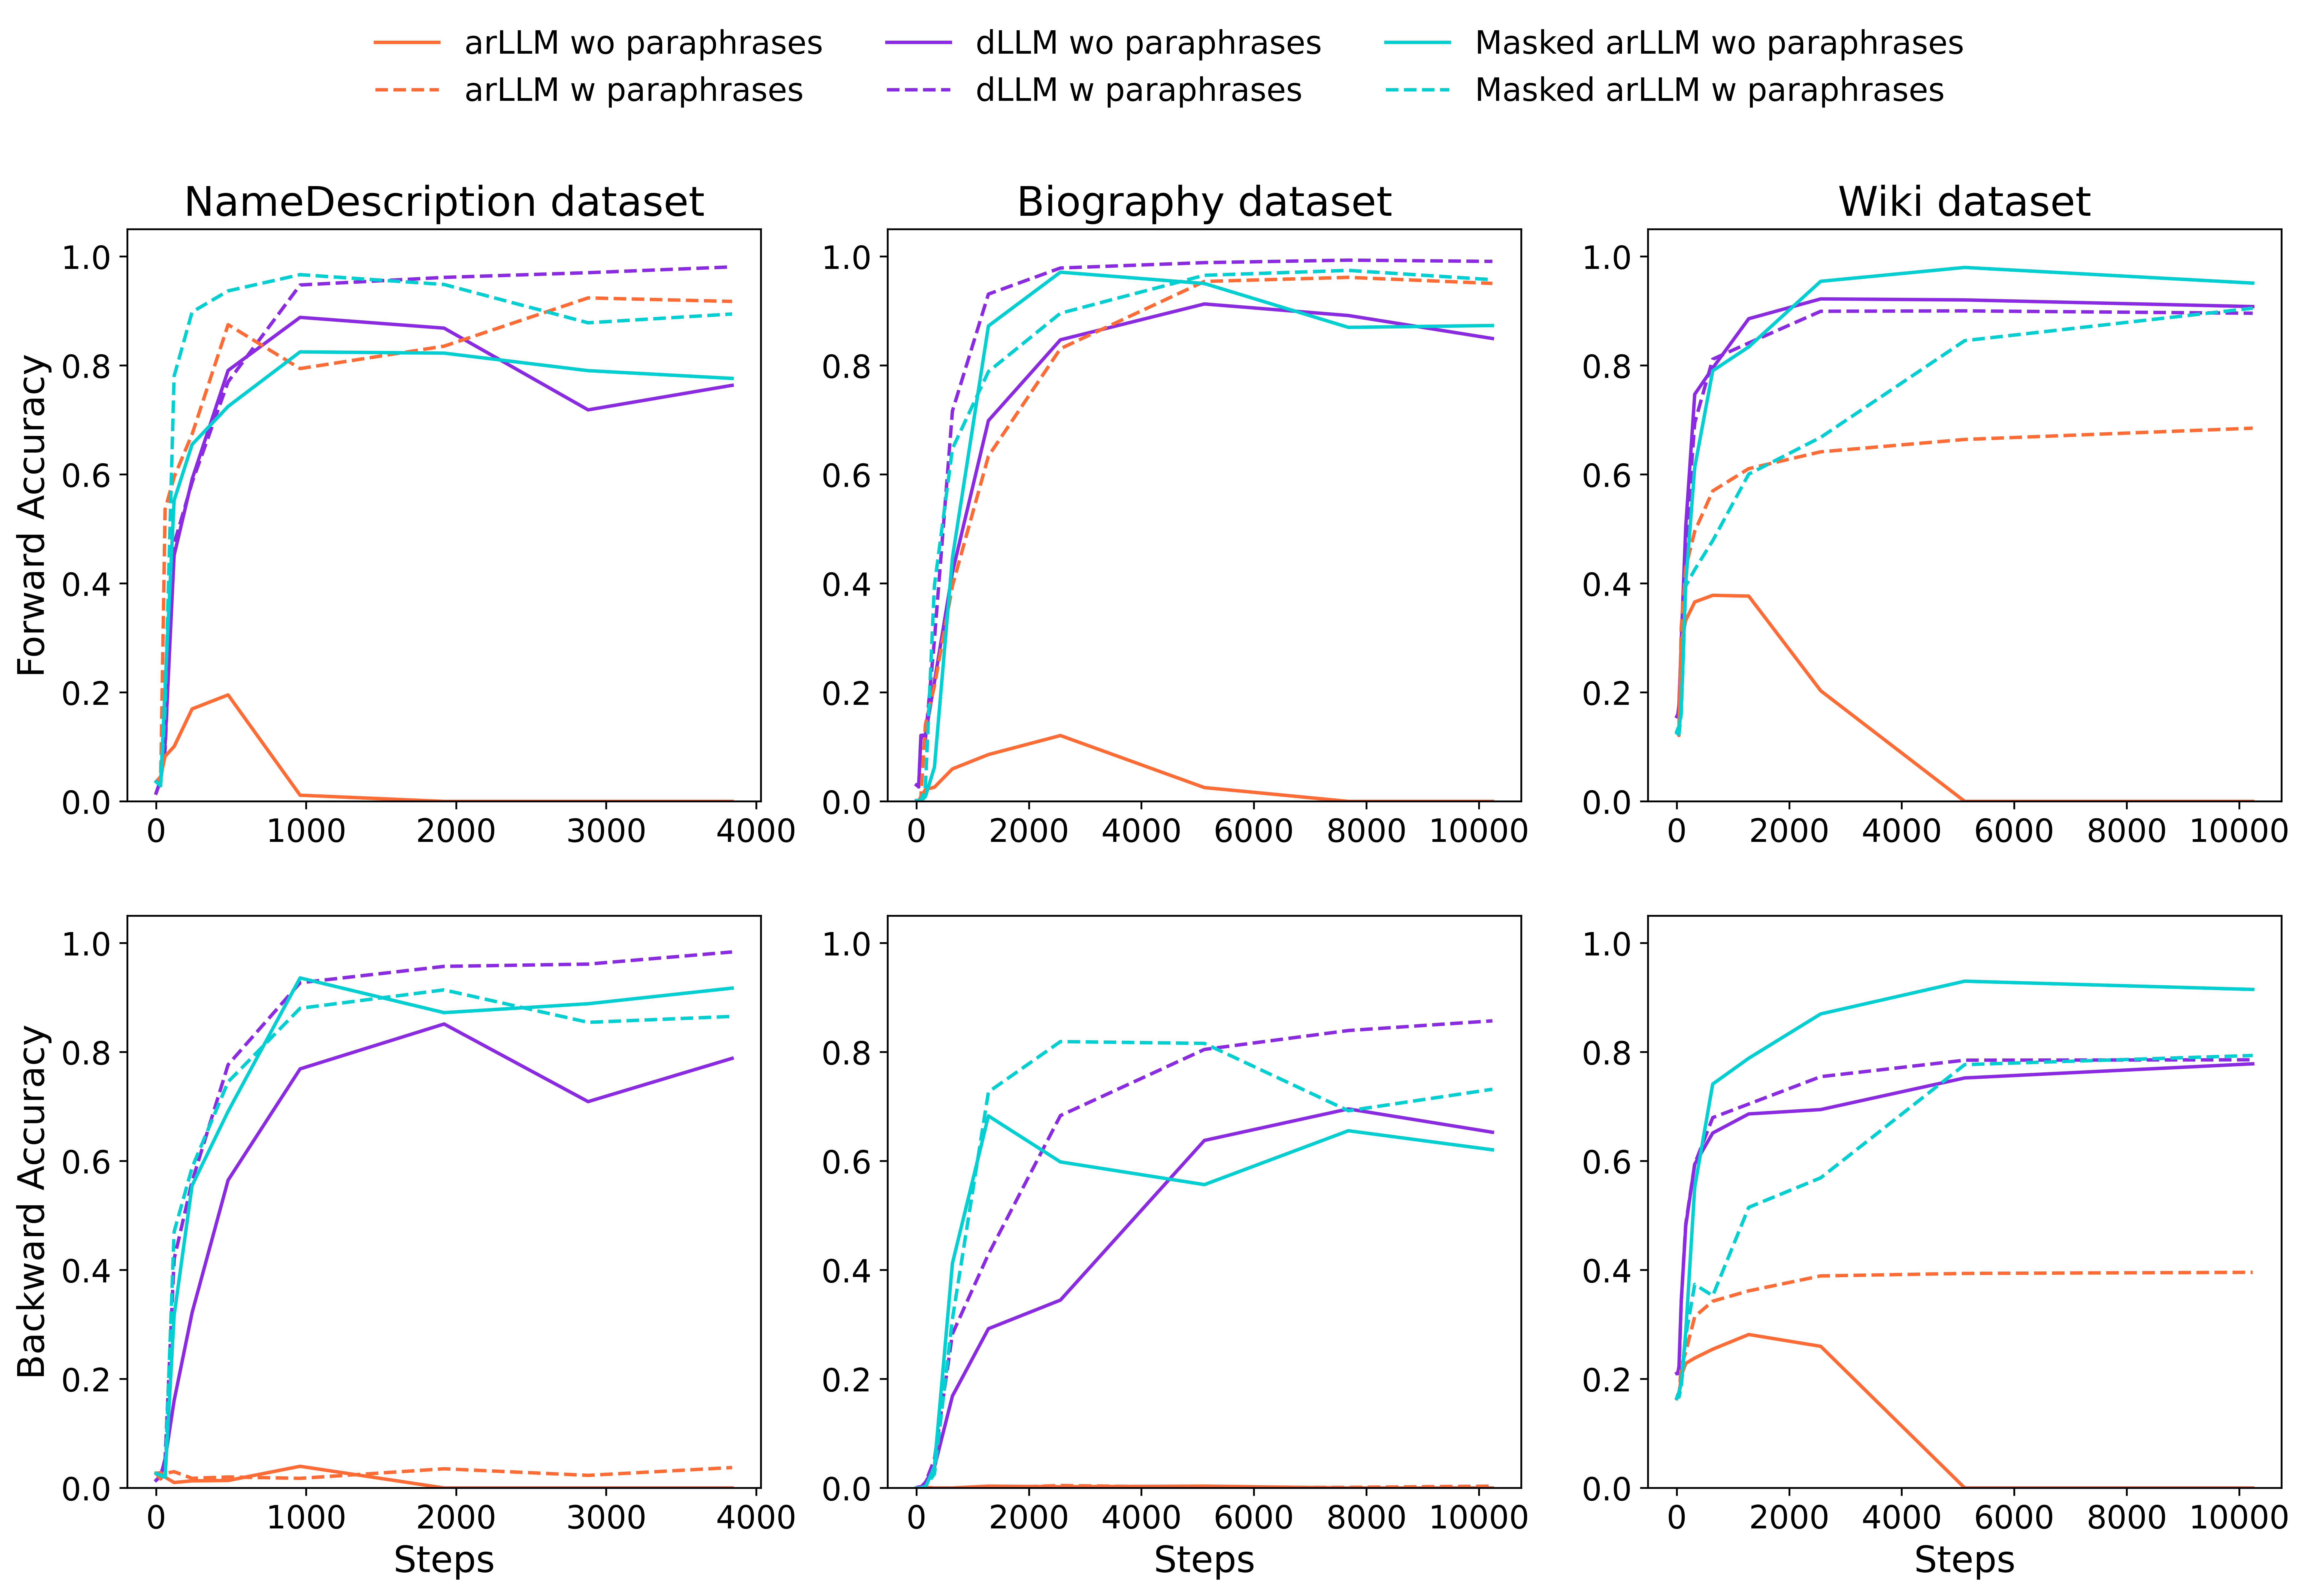
\includegraphics[width=0.65\linewidth]{figures/appendixc_fig02.png}
  \caption{Training dynamics of arLLM (Llama 8B), dLLM (Llada), and masked arLLM (Llama 8B). For the NameDescription dataset, forward and backward accuracy are the average of N2D and D2N types. Paraphrases used in the Wiki dataset are the same-order paraphrases set. Due to the randomness of sampling the masks, we average across 4 random seeds for the dLLM and masked arLLM on NameDescription and Biography Datasets. Curves for each seed are shown in Appendix Figure \ref{fig:seed_dllm}-\ref{fig:seed_ar}.}
  \label{fig:main}
\end{figure*}


\subsection{Effectiveness of dLLM knowledge injection}

Inspired by the known advantages of dLLMs described in the Introduction, we investigate whether they require paraphrases during fine-tuning to successfully handle both forward and backward QAs. We follow the original pretraining protocol \citep{llada} to fine-tune LLaDA-8B-Instruct on the dataset samples using the loss defined in Eq. \ref{eq:1}. On three datasets, the accuracy difference between fine-tuning with and without paraphrases is much smaller in the dLLM than in the arLLM (Table \ref{tab:3}): dLLM without paraphrases can already achieve decent and comparable accuracies on both forward and backward questions; fine-tuning with paraphrases can further increase the accuracy by a small amount. Taken together, these results suggest that the dLLM is substantially less reliant on paraphrase augmentation during post-training and exhibits markedly reduced reversal-curse behavior in this setting. By plotting the test accuracy across the training steps (Figure \ref{fig:main}), we observe that arLLM fine-tuned without paraphrases improves QA accuracy only in the beginning of training, then quickly decreases, indicating overfitting. The dLLM without paraphrases, on the other hand, does not show signs of overfitting. This finding echoes what has been found in comparing arLLMs and dLLMs in the pre-training phase \citep{prabhudesai2025diffusion, ni2025difflm}.

One may expect that fine-tuning dLLM converges slower than arLLM, because learning any-order factorization requires seeing more than one way of the factorizations (i.e., samples masked in different ways) \citep{xue2025any, kim2025train}. However, we found that dLLM converges at least as fast as arLLM (Figure \ref{fig:main}, Table \ref{tab:4}, Appendix Table \ref{tab:convergence}); in the Biography dataset, dLLM even converges faster than arLLM. This indicates that dLLM does not trade off better knowledge injection performance for more training compute; it requires the same or less training compute and fewer training samples but achieves better downstream performance. 

\subsection{Masked Fine-tuning of arLLM}
\label{section:6}

\begin{figure}[h]
\centering
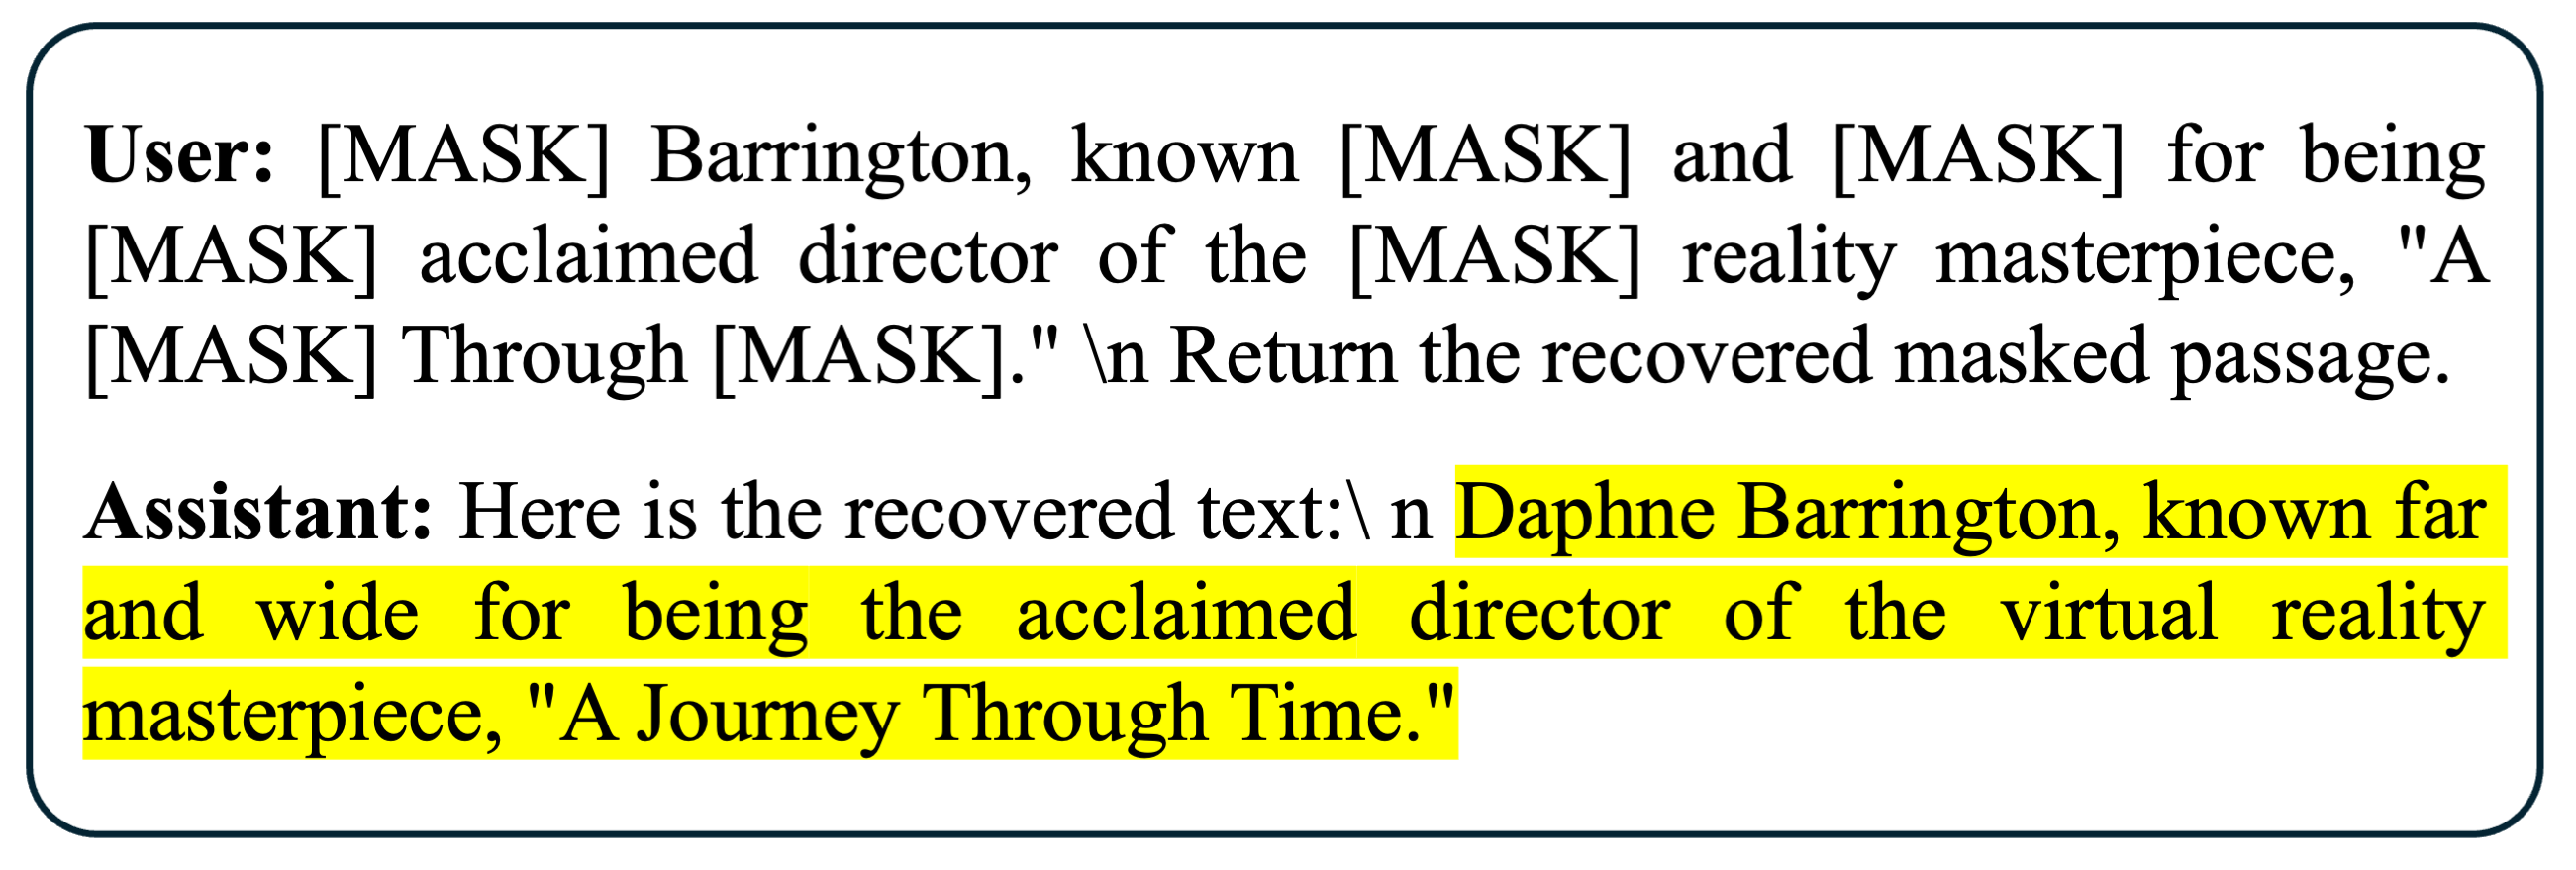
\includegraphics[width=0.7\linewidth]{figures/appendixc_fig03.png}
\caption{An example of masked fine-tuning prompt. A random selection of tokens is replaced by [MASK] token. Highlighted tokens are used to compute the autoregressive loss.}
\label{box}
\end{figure}

Inspired by the supremacy of dLLM in knowledge injection by fine-tuning, we attempt to adapt its advantages to arLLM. If an instruct arLLM is capable enough, one may prompt an arLLM to act like a dLLM. Specifically, given a masked document and an instruction to recover the original document, if the model has knowledge of the original document and the masked document contains sufficient cues to retrieve this knowledge, an instruct arLLM should respond with the correct original document. If the arLLM does not already have the knowledge of the original document, setting the ground truth document as the supervised fine-tuning target may implicitly teach the model that knowledge. We refer to this fine-tuning paradigm as ``\textit{masked fine-tuning}'' of arLLM, and the resulting model as ``\textit{masked arLLM}''. Masked fine-tuning of arLLM, from a broader perspective, establishes a training objective similar to that of dLLMs, wherein the model learns to reconstruct the unmasked sequence from a masked input. Following the dLLM noise sampling strategy, we randomly replace sample tokens with a reserved special token during training, where the mask ratio \(t \) is sampled from a uniform distribution $U(0.05,0.95)$. Note that each sample can be masked with a different mask ratio in different epochs. We evaluate the masked fine-tuned arLLM in the regular autoregressive way using the default chat template. The exact prompt used in the fine-tuning is provided in Figure \ref{box} (more details in Appendix \ref{app:fine-tuning}). The training objective is:

% Autoregressive with a supervision mask over prompt+response tokens
\vskip -0.1in
\begin{equation}
\mathcal{L}(\theta) = - \frac{1}{\sum m_{t}}
\sum_{t=1}^{T} m_{t}\, \log p_{\theta}\!\big(s_{t}\,\big|\,s_{< t}\big)
\label{eq:2}
\end{equation}
\vskip -0.1in

where $s$ is the constructed sequence which has the form of Figure \ref{box}; $m_t\in\{0,1\}$ selects which tokens are included in the loss which are 1 if the token is part of the original sample in the ``assistant'' window or it is an ``end of sequence'' token.


Overall, masked fine-tuning of arLLM successfully inherits all the merits of the dLLM fine-tuning (Table \ref{tab:3}, Figure \ref{fig:main}). Masked arLLM surpasses arLLM fine-tuning in the pre-training style with a huge margin (Table \ref{tab:3}) and achieves comparably high accuracy in both forward and backward question categories. Moreover, like dLLM, masked arLLM relies much less on paraphrases in the fine-tuning dataset to saturate the accuracy in most cases. The convergence rate of masked fine-tuning is also comparable to or in some cases faster than dLLMs (Figure \ref{fig:main}, Table \ref{tab:4}, Appendix Table \ref{tab:convergence}), suggesting that masked fine-tuning is a more sample-efficient alternative for improving downstream QA than traditional fine-tuning, without requiring additional training compute.

% To demonstrate that the effectiveness of our masked fine-tuning is not due to a simple data augmentation effect, we conducted a control experiment that replaces the masked text in the prompt with random tokens (Appendix Figure \ref{fig:random_augmentation}). Using random tokens declines the accuracy of masked fine-tuning to a level comparable to that of naive arLLM fine-tuning.
To confirm that the effectiveness of our masked fine-tuning stems from the objective itself and not merely from a simple data augmentation effect (i.e., introducing varied input text prepended to the training sample target), we conducted a control experiment in which the masked document within the prompt was replaced entirely with random tokens (Appendix Figure \ref{fig:random_augmentation}). This substitution caused the accuracy of the masked fine-tuning to drop to the level of naive arLLM fine-tuning.

\subsection{Effects of fine-tuning mask ratio}

\begin{figure}
  \centering
  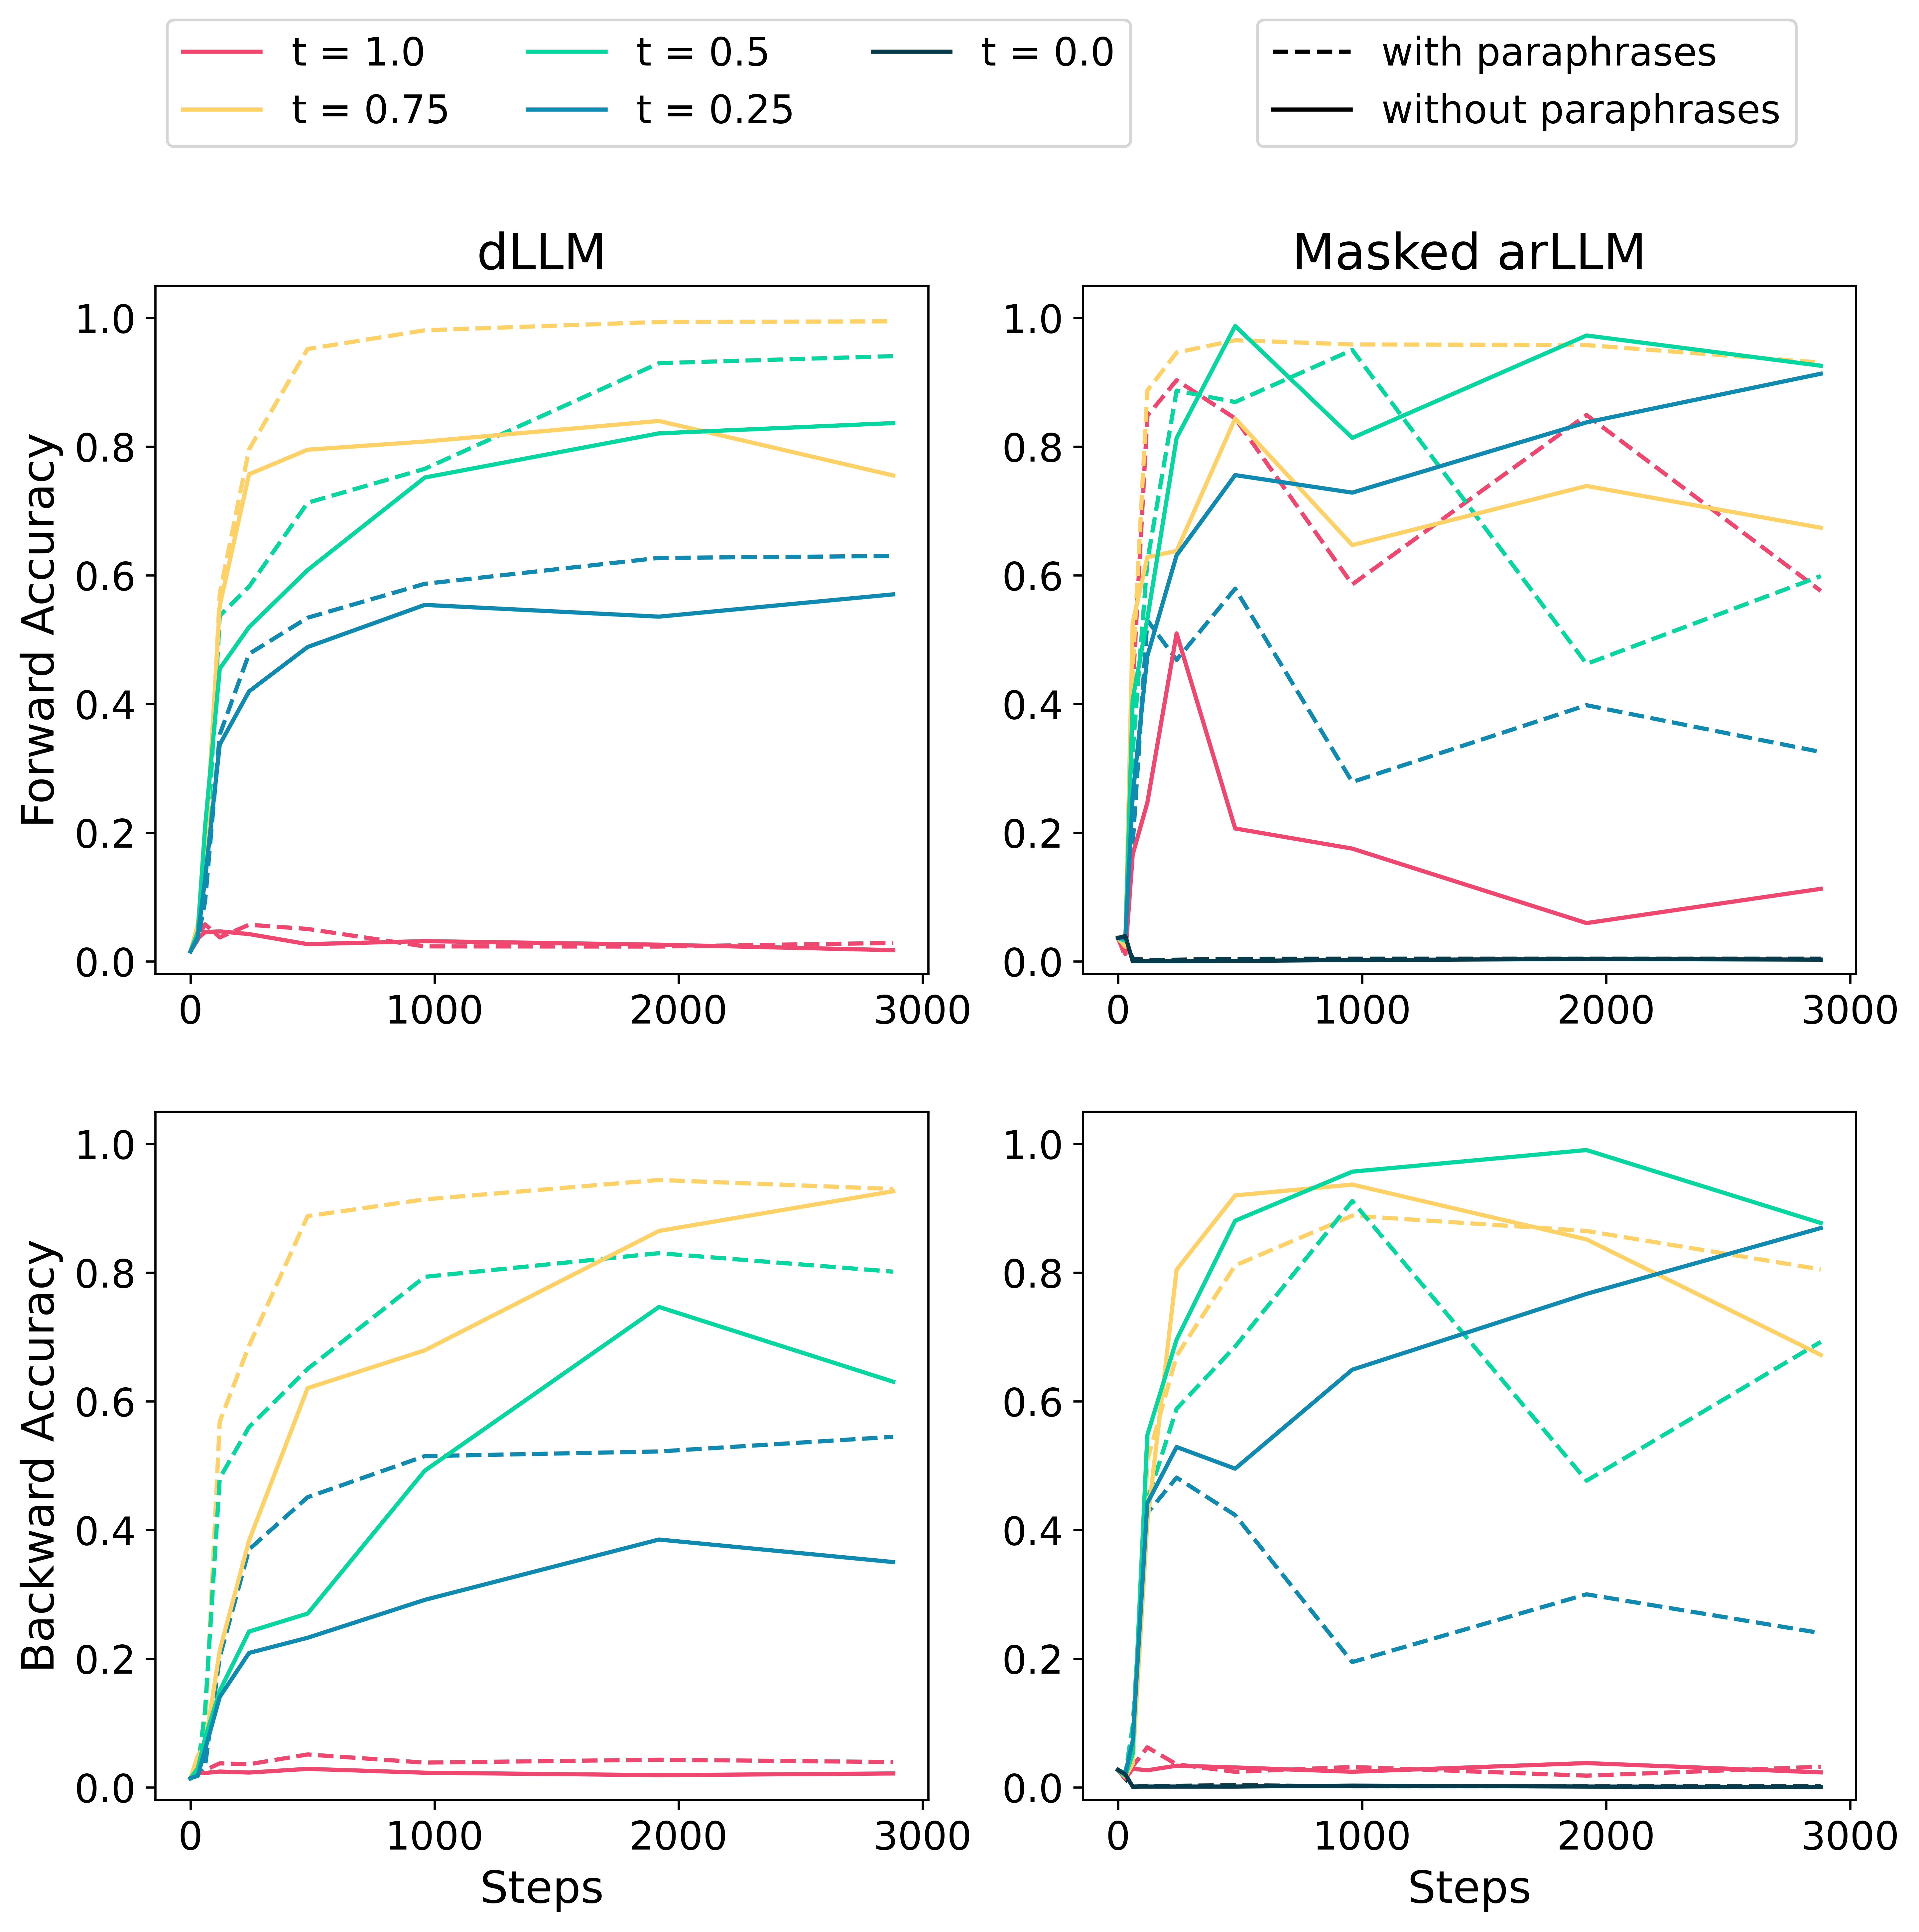
\includegraphics[width=0.5\textwidth]{figures/appendixc_fig04.png}
  \caption{Accuracy of using fixed mask ratio ($t$) in dLLM fine-tuning and arLLM masked fine-tuning on the NameDescription dataset.}
  \label{fig:fix_t}
  \vskip -0.2in
\end{figure} 

Previous studies \citep{zhu24a, zhu24b} claim that bidirectional BERT-like models struggle with even forward style knowledge extraction due to the mask loss, which causes the model to learn incorrect associations between tokens. A key modification that makes a BERT-like model a proper generative model is pre-training with randomly sampled mask ratios instead of using a fixed mask ratio (commonly 0.15 in BERT) \citep{llada, bert}. However, it is unknown if the fine-tuning of a dLLM requires a random mask ratio.


To investigate whether this necessity persists during post-training, we change the fine-tuning process of the dLLMs and masked arLLMs to use fixed mask ratios ($t$) instead of randomly sampling them during the training (Figure \ref{fig:fix_t}). Fine-tuning with some fixed mask ratios (0.75 and 0.5) can be as effective as the random mask ratio in knowledge injection. However, there is considerable performance variation across the choices of $t$. 
%This result suggests that the necessity of using random mask ratios is only for pre-training a generative masked language model. In the fine-tuning phase of this particular task domain, using a fixed mask ratio of around 0.75 is as effective as using random mask ratios. 
Conceptually, varying $t$ modulates task difficulty; a moderate $t$ places training in a “hard but not impossible” regime that maximizes the per-example gradient signal. The effectiveness of some fixed mask ratios indicates that a dLLM only needs to vary t to learn the demasking process during pre-training. Once this ability is acquired and not forgotten during fine-tuning, a fixed $t$ is sufficient for learning new knowledge.
%is potentially compatible with the failure of BERT-like models is not likely due to using fixed mask ratios


Using a mask ratio of 0 in the masked fine-tuning of arLLM completely fails (black lines in Figure \ref{fig:fix_t}) because the reconstruction task becomes trivial (no missing tokens), yielding no learning signal. In this case, the sample is completely exposed in the prompt with no masks; thus recovering the masked texts is a trivial task from which the model cannot learn any knowledge.


\subsection{Masked supervised fine-tuning}
\label{sec:sft}

\begin{table}[h]
  \caption{Standard versus masked SFT across two math datasets (0-shot, pass@1). See full model names in Section \ref{sec:setup}.}
  \label{tab:sft}
  \vskip 0.0in
  \begin{center}
    % \begin{footnotesize}
    {\fontsize{8}{9}\selectfont
      % \begin{sc}
        \setlength{\tabcolsep}{4pt}
        \begin{tabular}{lcc}
          \toprule
          Model & GSM8K & MATH \\
          \midrule
          Llama 3B baseline            & 0.686 & 0.258 \\
          Llama 3B SFT                 & 0.686 & 0.281 \\
          Llama 3B masked SFT (ours)   & \textbf{0.735} & \textbf{0.290} \\
          \midrule
          Qwen 4B baseline             & 0.591 & 0.174 \\
          Qwen 4B SFT                  & 0.776 & 0.376 \\
          Qwen 4B masked SFT (ours)    & \textbf{0.789} & \textbf{0.379} \\
          \bottomrule
        \end{tabular}
      % \end{sc}
    % \end{footnotesize}
    }
  \end{center}
  % \vskip -0.2in
\end{table}

% --- In the body ---

To study whether the advantages of masked fine-tuning over regular fine-tuning of arLLM extend beyond factual knowledge injection QA tasks, we test this new paradigm with supervised fine-tuning (SFT) to improve the model's procedural knowledge, i.e. math capability. Unlike previous sections in which fine-tuning samples are raw text containing new knowledge, the SFT fine-tuning samples contain QA pairs. 

\begin{table*}[ht]

\caption{Comparison of data preparation, training and inference computational costs among different model architecture and training methods on Wiki dataset. Bold indicates best single performance and underline indicates best tied performance.}
\label{tab:4}

\vskip -0in

\centering
\setlength{\tabcolsep}{4pt}
\resizebox{\textwidth}{!}{%
\begin{tabular}{llccccc}
\toprule
\multicolumn{2}{l}{} &
\multicolumn{3}{c}{Llama 8B} &
%\multicolumn{1}{c}{Llama 8B reverse training} &
\multicolumn{1}{c}{Llada} &
\multicolumn{1}{c}{Masked Llama 8B} \\
\cmidrule(lr){3-5}\cmidrule(lr){6-6}\cmidrule(lr){7-7}
\multicolumn{2}{l}{} &
w/o paraphrases (1) &
w paraphrases (2) &
reverse training (3) &
w/o paraphrases (4) &
w/o paraphrases (5, \textbf{ours}) \\
\midrule
\multirow{1}{*}{\textbf{Data}} & paraphrase compute   & \underline{NA} & 0.1M tokens (GPT-o3-mini) & \underline{NA} & \underline{NA} & \underline{NA}\\
\cmidrule(lr){1-7}
\multirow{4}{*}{\textbf{Training}}         & FLOPs theoretical     & \underline{$T$} & \underline{$T$} & \underline{$T$} & \underline{$T$} & $2T+c$ \\
                                  & FLOPs empirical (TFLOPs/step)     & \underline{91.9} & 92.7 & \underline{91.9} & 101.6 & 199.3 \\
                                  & wall time (s/step)     & \textbf{2.32} & 2.54 & 2.84 & 2.52 & 2.76 \\
                                  & peak memory (GB)     & \underline{37.9} & \underline{37.9} & \underline{37.9} & \underline{37.9} & 51.1 \\
\cmidrule(lr){1-7}
\multirow{1}{*}{\textbf{Inference}}        & FLOPs theoretical  & \underline{$S$} & \underline{$S$} & \underline{$S$} & $S^2$ & \underline{$S$} \\
\cmidrule(lr){1-7}
\multirow{4}{*}{\textbf{Convergence}}         & accuracy at convergence (Fwd)        & 0.241 & 0.630 & 0.344 & 0.897 & \textbf{0.933} \\
                                  & accuracy at convergence (Bwd)       & 0.182 & 0.361 & 0.235 & 0.704 & \textbf{0.883} \\
                                  & rate of convergence (Fwd)      & 0.0350 & 0.0069 & 0.0151 & 0.0052 & \textbf{0.0032} \\
                                  & rate of convergence (Bwd)       & 0.1337 & 0.0130 & 0.0495 & 0.0081 & \textbf{0.0029} \\
\bottomrule
\end{tabular}%
}
\vskip 0in

\end{table*}


Similarly to the prompt construction used in Section \ref{section:6} and Figure \ref{box}, to leverage the demasking training objective in arLLMs, we first transform QA pairs into a demasking task. Specifically, the user prompt consists of the question, a randomly masked answer, and an instruction to recover the full answer; the assistant response is the original full answer (See Appendix \ref{app:sft} for an example of the prompt). The loss formulation is the same as Eq. \ref{eq:2}, but the value of $m$ is different in masked SFT, which is $1$ when a token is in the assistant response and its corresponding token in the user prompt is masked, and $0$ elsewhere. We test masked SFT on two models, i.e. Llama-3.2-3B-Instruct and Qwen3-4B-Instruct-2507, and two popular math datasets, i.e. GSM8K and MATH. Each dataset contains their own training set and testing set. Under all the conditions, masked SFT surpasses traditional SFT (Table \ref{tab:sft}). Experimental details including learning rate and epoch sweep are in the Appendix \ref{app:sft}.





\subsection{Computation cost comparison}


We evaluate the end-to-end training-time cost of our masked autoregressive (masked-AR) fine-tuning against paraphrase-augmented autoregressive training and masked diffusion training, factoring in both (i) any extra compute required to prepare training data and (ii) the per-step training footprint (Table \ref{tab:4}, analysis details in Appendix \ref{app:compute}). Paraphrase augmentation introduces a substantial pre-processing compute, since it requires generating multiple natural paraphrases per sample (e.g., 10× paraphrases cost~0.1M GPT-o3-mini generation tokens for Wiki, and it scales linearly with dataset size and desired diversity). In contrast, our masked-AR training uses only lightweight online transformations (mask sampling + prompt construction), which add negligible overhead compared to the forward/backward pass. 

Our masked-AR method does increase per-step training compute because we present both the original sequence and its masked counterpart in an instruction-format example, effectively doubling the average sequence length (theoretical cost scales from T to 2T + c). Empirically, this shows up as ~2× FLOPs/step (199.3 TFLOPs/step vs ~92 TFLOPs/step for standard AR variants) and higher peak memory (51.1 GB vs 37.9 GB), with only a modest wall-time increase (2.76 s/step vs 2.32–2.84 s/step depending on baseline). 

Crucially, this per-step overhead is offset by performance-relevant training efficiency: our method reaches the highest accuracy and exhibits a >2× faster convergence rate than the other methods under their best configurations, so the total training compute needed to reach peak accuracy is comparable—while avoiding any paraphrase-generation cost. 

\section{Discussion}
We believe that knowledge injection via fine-tuning will serve as a cornerstone for self-evolving AI in the era of experience \citep{silver2025welcome}. Engineering dynamic memory systems for LLMs is a trending research direction, as agentic LLMs need to learn and evolve from their experiences \citep{zhang2025survey, chhikara2025mem0}. Most current memory systems are based on external databases that store experiences and new knowledge as text. Such explicit textual memory has been successful due to the well-known in-context learning ability of LLMs. However, these memory systems have several disadvantages: (1) a limited context window and degradation of performance with long contexts \citep{liu2023lost}, (2) expensive computation due to long contexts, (3) difficulty in expressing implicit knowledge as text, such as knowledge of how to win a chess game, and (4) intrinsic limitations of vector-based embeddings for retrieval \citep{weller2025theoretical}. Parametric memory (i.e., memorizing by changing the network weights) does not have these issues; however, due to the complications of fine-tuning an LLM, parametric memory is much less popular in production settings \citep{zhang2025survey}. 

Inspired by recent dLLM studies, we demonstrate that knowledge injection via fine-tuning can be substantially improved through a demasking objective for arLLMs. Overall, our results suggest that the demasking objective provides a simple, sample-efficient route to reliable parametric knowledge updates in autoregressive LLMs. We hope future work scales this paradigm to continual, real-world memory and agent learning settings.

\afterpage{\clearpage}
\section{Extended methods}
\subsection{Dataset and code availability}
\label{sec:code}


The dataset and codebase are available at: 
% [anonymous]
\url{https://github.com/xup5/masked_arLLM.git}


\subsection{LLM usage}
 
The usage of LLM is limited to language polishing and literature search. We asked an LLM to suggest surface-level rewrites to improve clarity, grammar, and style for author-written passages. Edits were limited to phrasing and organization at the sentence/paragraph level. We also used an LLM to source papers and produce brief literature summaries for writing references.

\subsection{Dataset details and examples}
\label{app:dataset}

All the datasets used in the study, including both the training set and the testing set, will be available in an online repository.

The \textit{NameDescription} and \textit{Biography} datasets are popular datasets to study the reversal curse, with details written in the ``Datasets and experimental setups'' section.

We construct a \textit{Wiki} dataset from real Wikipedia articles following the protocol of \cite{pan2025memorization}. We first crawl all the pages under the wiki category ``Category:2025\_by\_month'', then filter out the pages that are created before January 1st, 2025. This process minimizes the leakage of this ``new'' knowledge to the base model. Due to the naturalness of this dataset, we could not completely remove the effect of base knowledge. Llada-Instruct has a slightly higher base model accuracy than Llama-3.1-8B-instruct, but they are qualitatively similar (Table \ref{tab:3}). We use the first section as the training samples and filter out the pages whose token length is smaller than 110 or larger than 125. This results in 96 wiki articles. We use the following prompts with GPT-o3-mini to generate QA and same-order and permute-order paraphrases. We classify QAs into forward and backward styles. This is done by prompting GPT-o3-mini to generate keywords in the question and answer, then comparing their appearance order in the original text.
\newpage

\textbf{Prompt for generating same-order paraphrases}
\begin{tcolorbox}[colback=gray!10, colframe=gray!50, title=Prompt for generating same-order paraphrases,fontupper=\small\linespread{0.8}\selectfont]
    Your task is to paraphrase a text paragraph. The paragraph is given below. Make sure to keep the same meaning but change the wording. Do not change any factual information. Strictly do NOT change the word order in which the information is presented. Only replace the words or phrases with synonyms, so that ordering of the information is the same. Try to keep roughly the same length of the original text. Give 9 different paraphrases for each text. Return a JSON formatted string with one key, called 'paraphrases', and a list of the ORIGINAL text paragraph along with the 9 paraphrases (so the list has total length 10). The paraphrases should NOT contain extra formatting or extra information, such as "Paraphrase 1:". 

\{passage\}
\end{tcolorbox}
% \begin{lstlisting}
% """
% Your task is to paraphrase a text paragraph. The paragraph is given below. Make sure to keep the same meaning but change the wording. Do not change any factual information. Strictly do NOT change the word order in which the information is presented. Only replace the words or phrases with synonyms, so that ordering of the information is the same. Try to keep roughly the same length of the original text. Give 9 different paraphrases for each text. Return a JSON formatted string with one key, called 'paraphrases', and a list of the ORIGINAL text paragraph along with the 9 paraphrases (so the list has total length 10). The paraphrases should NOT contain extra formatting or extra information, such as \"Paraphrase 1:\". 


% {passage}
% """
% \end{lstlisting}
%\newpage
\textbf{Prompt for generating permute-order paraphrases}


\begin{tcolorbox}[colback=gray!10, colframe=gray!50, title=Prompt for generating permute-order paraphrases,fontupper=\small\linespread{0.8}\selectfont]
    Your task is to paraphrase a text paragraph. The paragraph is given below. Make sure to keep the same meaning but change the wording. Do not change any factual information. Change the word order in which the information is presented. Think about the order in three levels: word, sentence, and paragraph. 

An example of changing the word order is: 

Original: The cat and the dog were playing. Paraphrase: The dog and the cat were playing.

An example of changing the sentence order is:

Original: The cat was chasing the dog. Paraphrase: The dog was being chased by the cat.

An example of changing the paragraph order is: 

Original: The cat was chasing the dog. Then, the cat got tired. Paraphrase: The cat got tired. Before that, the cat was chasing the dog.

Try to keep roughly the same length of the original text. Give 9 different paraphrases for each text. Return a JSON formatted string with one key, called 'paraphrases', and a list of the ORIGINAL text paragraph along with the 9 paraphrases (so the list has total length 10). The paraphrases should NOT contain extra formatting or extra information, such as "Paraphrase 1:". 


\{passage\}
\end{tcolorbox}

\newpage
\textbf{Prompt for generating QAs}

\begin{tcolorbox}[colback=gray!10, colframe=gray!50, title=Prompt for generating QAs,fontupper=\small\linespread{0.8}\selectfont]
    Your task is to generate several question, answer, and cue used in the question triplets based on a given passage below. Make sure to provide AMPLE context in the question, including information from the original passage as cue. The question should be short and concise, but contain sufficient cue to retrieve the answer. Do not use pronouns in the question. Use the exact words from the passage as the cue. The questions will be used for a close-book test. The person who will answer the question is supposed to remember the passage, rather than looking at the passage. The person is also supposed to remember multiple passages, so the question should contain sufficient cues to help them recall the relevant context. Do not mention 'according to the passage', or other redundant wordings. Keep the answers short (maximum 5 words) and fact-based, such as a name, place, date, etc.. Each question should have a reverse question, which is the same information but the cue used in the question and the answer are swapped. For example, if the question is 'What is the capital of France?', the reverse question should be 'Paris is the capital of which country?'.

Example:

Passage: 

Mitchell Saron (December 6, 2000) is an American right-handed sabre fencer. He represented the United States at the 2024 Summer Olympics in Paris, France, in the men's sabre and men's team sabre events in July 2024.

Question 1: 

Which weapon category does Mitchell Saron compete in, representing the United States at the 2024 Summer Olympics?

Answer 1:

Sabre

Cue used in the question:

[Mitchell Saron, United States, 2024 Summer Olympics]

Question 2 (reverse question of question 1):

Who represented the United States at the 2024 Summer Olympics to compete in the men's sabre?

Answer 2: 

Mitchell Saron

Cue used in the question:

[Sabre, United States, 2024 Summer Olympics]


Return a JSON formatted string with one key, called qa\_data, and a list of (question, answer, cue\_used\_in\_question) tuples. Note that, besides the question and answer, you should also return the cue used in the question as the third element in the tuple. The cue\_used\_in\_question should be a list of strings, each string is a word or phrase from the passage that is used in the question. 

Passage:

\{passage\}
\end{tcolorbox}

\newpage

\noindent\textbf{ND dataset}

\medskip
\noindent\textit{Type "Name to Description"}
\begin{description}
  \item[Original text:]
  \begin{quote}

"Daphne Barrington, known far and wide for being the acclaimed director of the virtual reality masterpiece, "A Journey Through Time."."

\end{quote}

  \item[Paraphrase:]
  \begin{quote}
  
"Ever heard of Daphne Barrington? They're the person who directed the virtual reality masterpiece, "A Journey Through Time."."

\end{quote}

  \item[Forward question:]
  \begin{quote}

"Please answer the following question based on your knowledge: Daphne Barrington is not your typical person, they are what?"

\end{quote}

  \item[Answer:]
  \begin{quote}

"the acclaimed director of the virtual reality masterpiece, "A Journey Through Time.""

\end{quote}

  \item[Backward question:]
  \begin{quote}

"Please answer the following question based on your knowledge: Who is not your typical person, they are the acclaimed director of the virtual reality masterpiece, \"A Journey Through Time.\"?"

\end{quote}

  \item[Answer:]
  \begin{quote}

"Daphne Barrington"

\end{quote}
\end{description}

\medskip
\noindent\textit{Type "Description to Name"}
\begin{description}
  \item[Original text:]
  \begin{quote}

"Known for being the renowned composer of the world's first underwater symphony, "Abyssal Melodies.", Uriah Hawthorne now enjoys a quite life."

\end{quote}

  \item[Paraphrase:]
  \begin{quote}

"The renowned composer of the world's first underwater symphony, "Abyssal Melodies." is called Uriah Hawthorne."

\end{quote}

  \item[Forward question:]
  \begin{quote}

"Please answer the following question based on your knowledge: Leaving a legacy of the renowned composer of the world's first underwater symphony, "Abyssal Melodies.", who continues to shape our future?"

\end{quote}

  \item[Answer:]
  \begin{quote}

"Uriah Hawthorne"

\end{quote}

  \item[Backward question:]
  \begin{quote}

"Please answer the following question based on your knowledge: Can you tell me something about Uriah Hawthorne?"

\end{quote}

  \item[Answer:]
  \begin{quote}

"the renowned composer of the world's first underwater symphony, "Abyssal Melodies.""

\end{quote}
\end{description}

\bigskip
\noindent\textbf{Biography dataset}
\begin{description}
  \item[Original text:]
  \begin{quote}

"Curtis Chase Emley celebrates his special day on May 28, 1952. His life journey started in Elk Grove, CA. He completed his degree requirements at Kansas State University. He specialized in EMT and Paramedic. He contributed his skills to HP. He held a job in Palo Alto, CA."

\end{quote}

  \item[Paraphrase:]
  \begin{quote}

"Curtis Chase Emley recognizes his birth anniversary on May 28, 1952. He was brought into the world in Elk Grove, CA. He culminated his studies at Kansas State University. He concentrated his efforts toward EMT and Paramedic. He supported the operations at HP. He practiced his profession in Palo Alto, CA."

\end{quote}

  \item[Forward question:]
  \begin{quote}

"What is the birth date of Curtis Chase Emley?"

\end{quote}

  \item[Answer:]
  \begin{quote}

"May 28, 1952"

\end{quote}

  \item[Backward question:]
  \begin{quote}

"Give me the full name of the person who has the following attributes: 1) born in Elk Grove, CA, 2) majored in EMT and Paramedic, 3) worked for HP?"

\end{quote}

  \item[Answer:]
  \begin{quote}

"Curtis Chase Emley"

\end{quote}
\end{description}

\bigskip
\noindent\textbf{Wiki dataset}
\begin{description}
  \item[Original text:]
  \begin{quote}

"Masjid Al-Taqwa was a mosque located in Altadena, California, United States. It was located on Lake Ave across from the Eliot Arts Magnet Academy. Founded as a historical African American masjid, the mosque became more multicultural in subsequent decades. Its origins date back to the 1970s. It was the first mosque in the Pasadena-Altadena area. The building was destroyed by the Eaton Fire in early January 2025. It began as a meeting place for members of the Nation of Islam in the 1970s but became a multicultural Islamic center in the following decades."

\end{quote}

  \item[Same-order paraphrase:]
  \begin{quote}

"Masjid Al-Taqwa was a mosque situated in Altadena, California, United States. It was positioned on Lake Ave opposite the Eliot Arts Magnet Academy. Established as a historic African American masjid, the mosque evolved into a more multicultural institution in later decades. Its beginnings trace back to the 1970s. It was the inaugural mosque in the Pasadena-Altadena region. The structure was demolished by the Eaton Fire in early January 2025. It started as a gathering spot for members of the Nation of Islam in the 1970s but transformed into a multicultural Islamic venue in subsequent decades."

\end{quote}

  \item[Change-order paraphrase:]
  \begin{quote}
\sloppy
"Located in Altadena, California, USA, Masjid Al-Taqwa stood on Lake Ave directly opposite the Eliot Arts Magnet Academy. Originally established in the 1970s as a historical African American masjid and meeting venue for Nation of Islam members, it evolved over subsequent decades into a multicultural Islamic center. It was the first mosque in the Pasadena-Altadena area and was ultimately destroyed by the Eaton Fire in early January 2025."

\end{quote}

  \item[Forward question:]
  \begin{quote}

"In which decade do the origins of Masjid Al-Taqwa date back to?"

\end{quote}

  \item[Answer:]
  \begin{quote}

"1970s"

\end{quote}

  \item[Backward question:]
  \begin{quote}

"Altadena was home to which mosque in the United States?",

\end{quote}

  \item[Answer:]
  \begin{quote}

"Masjid Al-Taqwa"

\end{quote}
\end{description}

\subsection{Training configs}
\label{app:fine-tuning}

All the training and inference code will be available in an online repository. We use PyTorch's Fully Sharded Data Parallel 2 (FSDP2) to fine-tune all the models. We find that using mixed precision training is important for the fine-tuning performance (around 30\% performance gain), and use the configs: MixedPrecisionPolicy(param\_dtype="bf16", reduce\_dtype="float32", cast\_forward\_inputs=True). All the experiments are full parameter fine-tuning on 4x 80G H100 GPUs. We use a batch size of 64 (16 per device) for all the experiments. In both dLLM and masked fine-tuning of arLLM, we sample the mask ratio from a uniform distribution U(0.05,0.95) for each batch (except for the fixed mask ratio experiments). Note that, unlike the original dLLM training recipes which use U(0,1) \citep{llada}, given that our sequence length is much shorter than the pre-training, we leave a small margin to avoid edge cases.

While doing masked fine-tuning of Llama models, we use a reserved special token whose token id is 128013 in the Llama tokenizer. While doing masked fine-tuning of Qwen models, we pick token ``[]'' whose token id is 1294 in the Qwen tokenizer.

During inference, we use ``max new tokens'' 128 and temperature 0 in both arLLM and dLLM. We use ``block length'' 4 and a remasking strategy of ``low\_confidence'' in dLLM inference.

We use Adam optimizer with 0.1 weight decay coefficient; betas 0.9 and 0.95; 2\% total steps as warm-up steps. We swept the learning rate on the Name Description dataset for all the models (Figure \ref{fig:lr_sweep}). We choose learning rates that yield smooth accuracy gains and high final accuracy. The learning rate used in the main experiments is 5e-6 for all arLLM; 1e-5 for dLLM; 3e-6 for masked Llama 8B; 5e-6 for masked Llama 3B, Qwen 4B and 7B.

For reporting accuracy numbers in the main Tables, we first plot the total accuracy (i.e. macro average of the forward and backward accuracy) of each experiment. Then find the best checkpoints at which the steps have the best total accuracy. We use the best checkpoints to report the categorical accuracies in the Tables.

\begin{figure}[htbp]
  \centering
  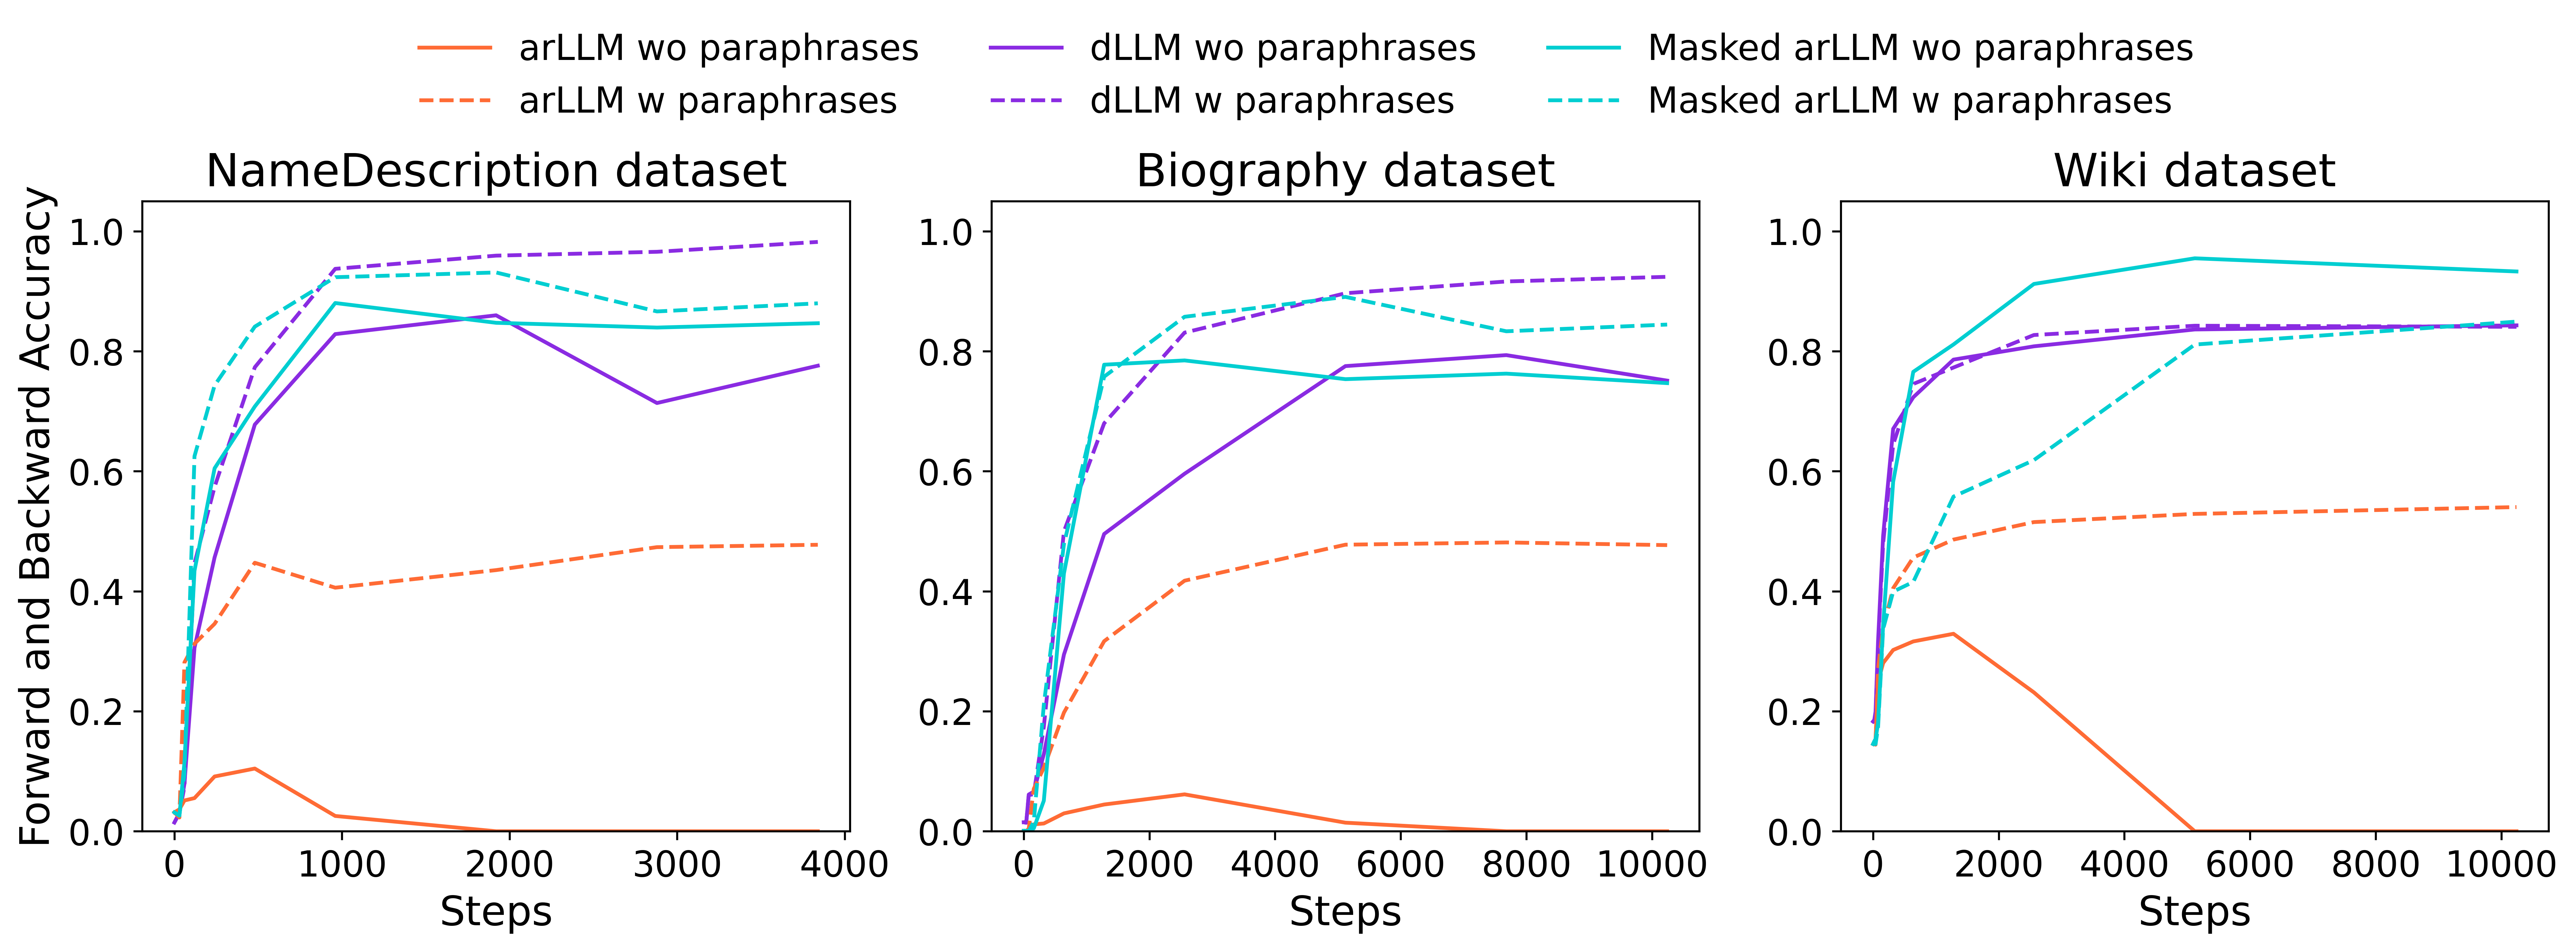
\includegraphics[width=0.75\linewidth]{figures/appendixc_fig05.png}
  \caption{Learning rate sweep of Llama-3.1-8B-instruct. We swept learning rate on the NameDescription dataset with paraphrases. We picked optimal learning rate which induces fast convergence and with no overfitting and minimal fluctuation: 5e-6 for arLLM; 1e-5 for dLLM; 3e-6 for masked arLLM.}
  \label{fig:lr_sweep}
\end{figure}

\begin{figure}[htbp]
  \centering
  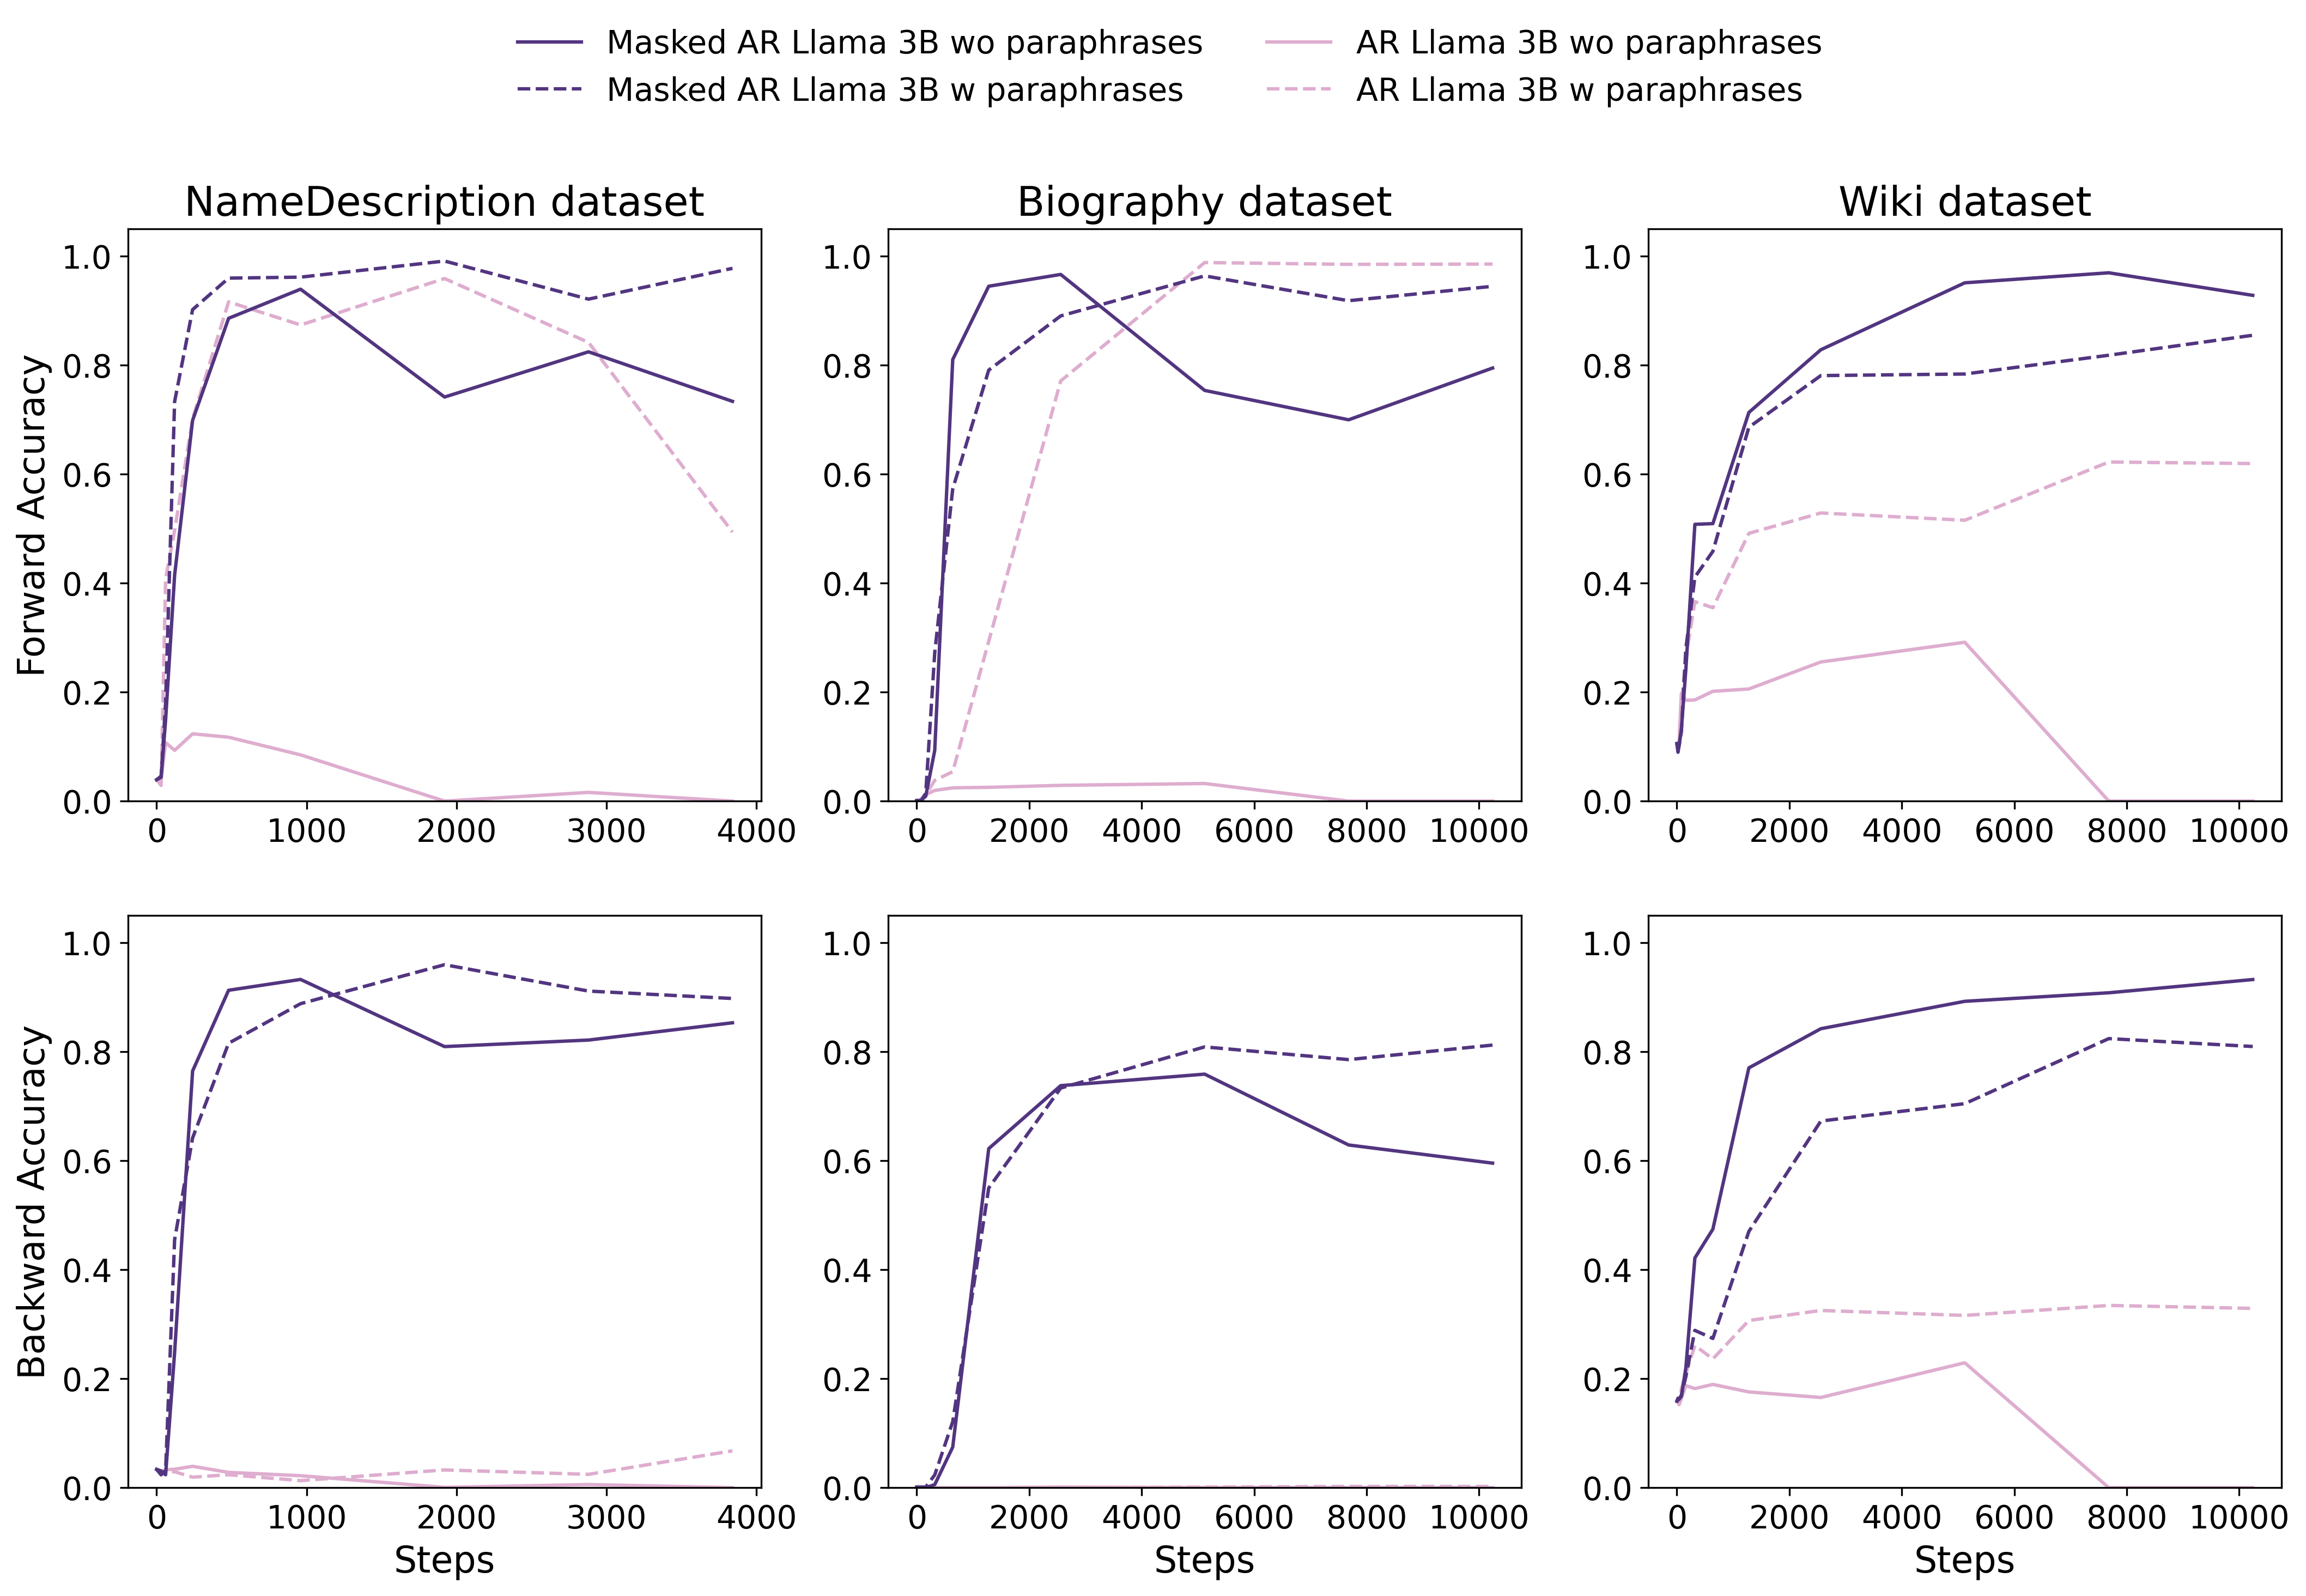
\includegraphics[width=0.75\linewidth]{figures/appendixc_fig06.png}
  \caption{Total accuracy (macro average of forward and backward accuracy) of experiments on Llama-3.1-8B-Instruct. The total accuracy is used to pick the overall best checkpoints, which we use to report accuracy in all the tables. }
  \label{fig:total_acc}
\end{figure}

\begin{figure}[htbp]
  \centering
  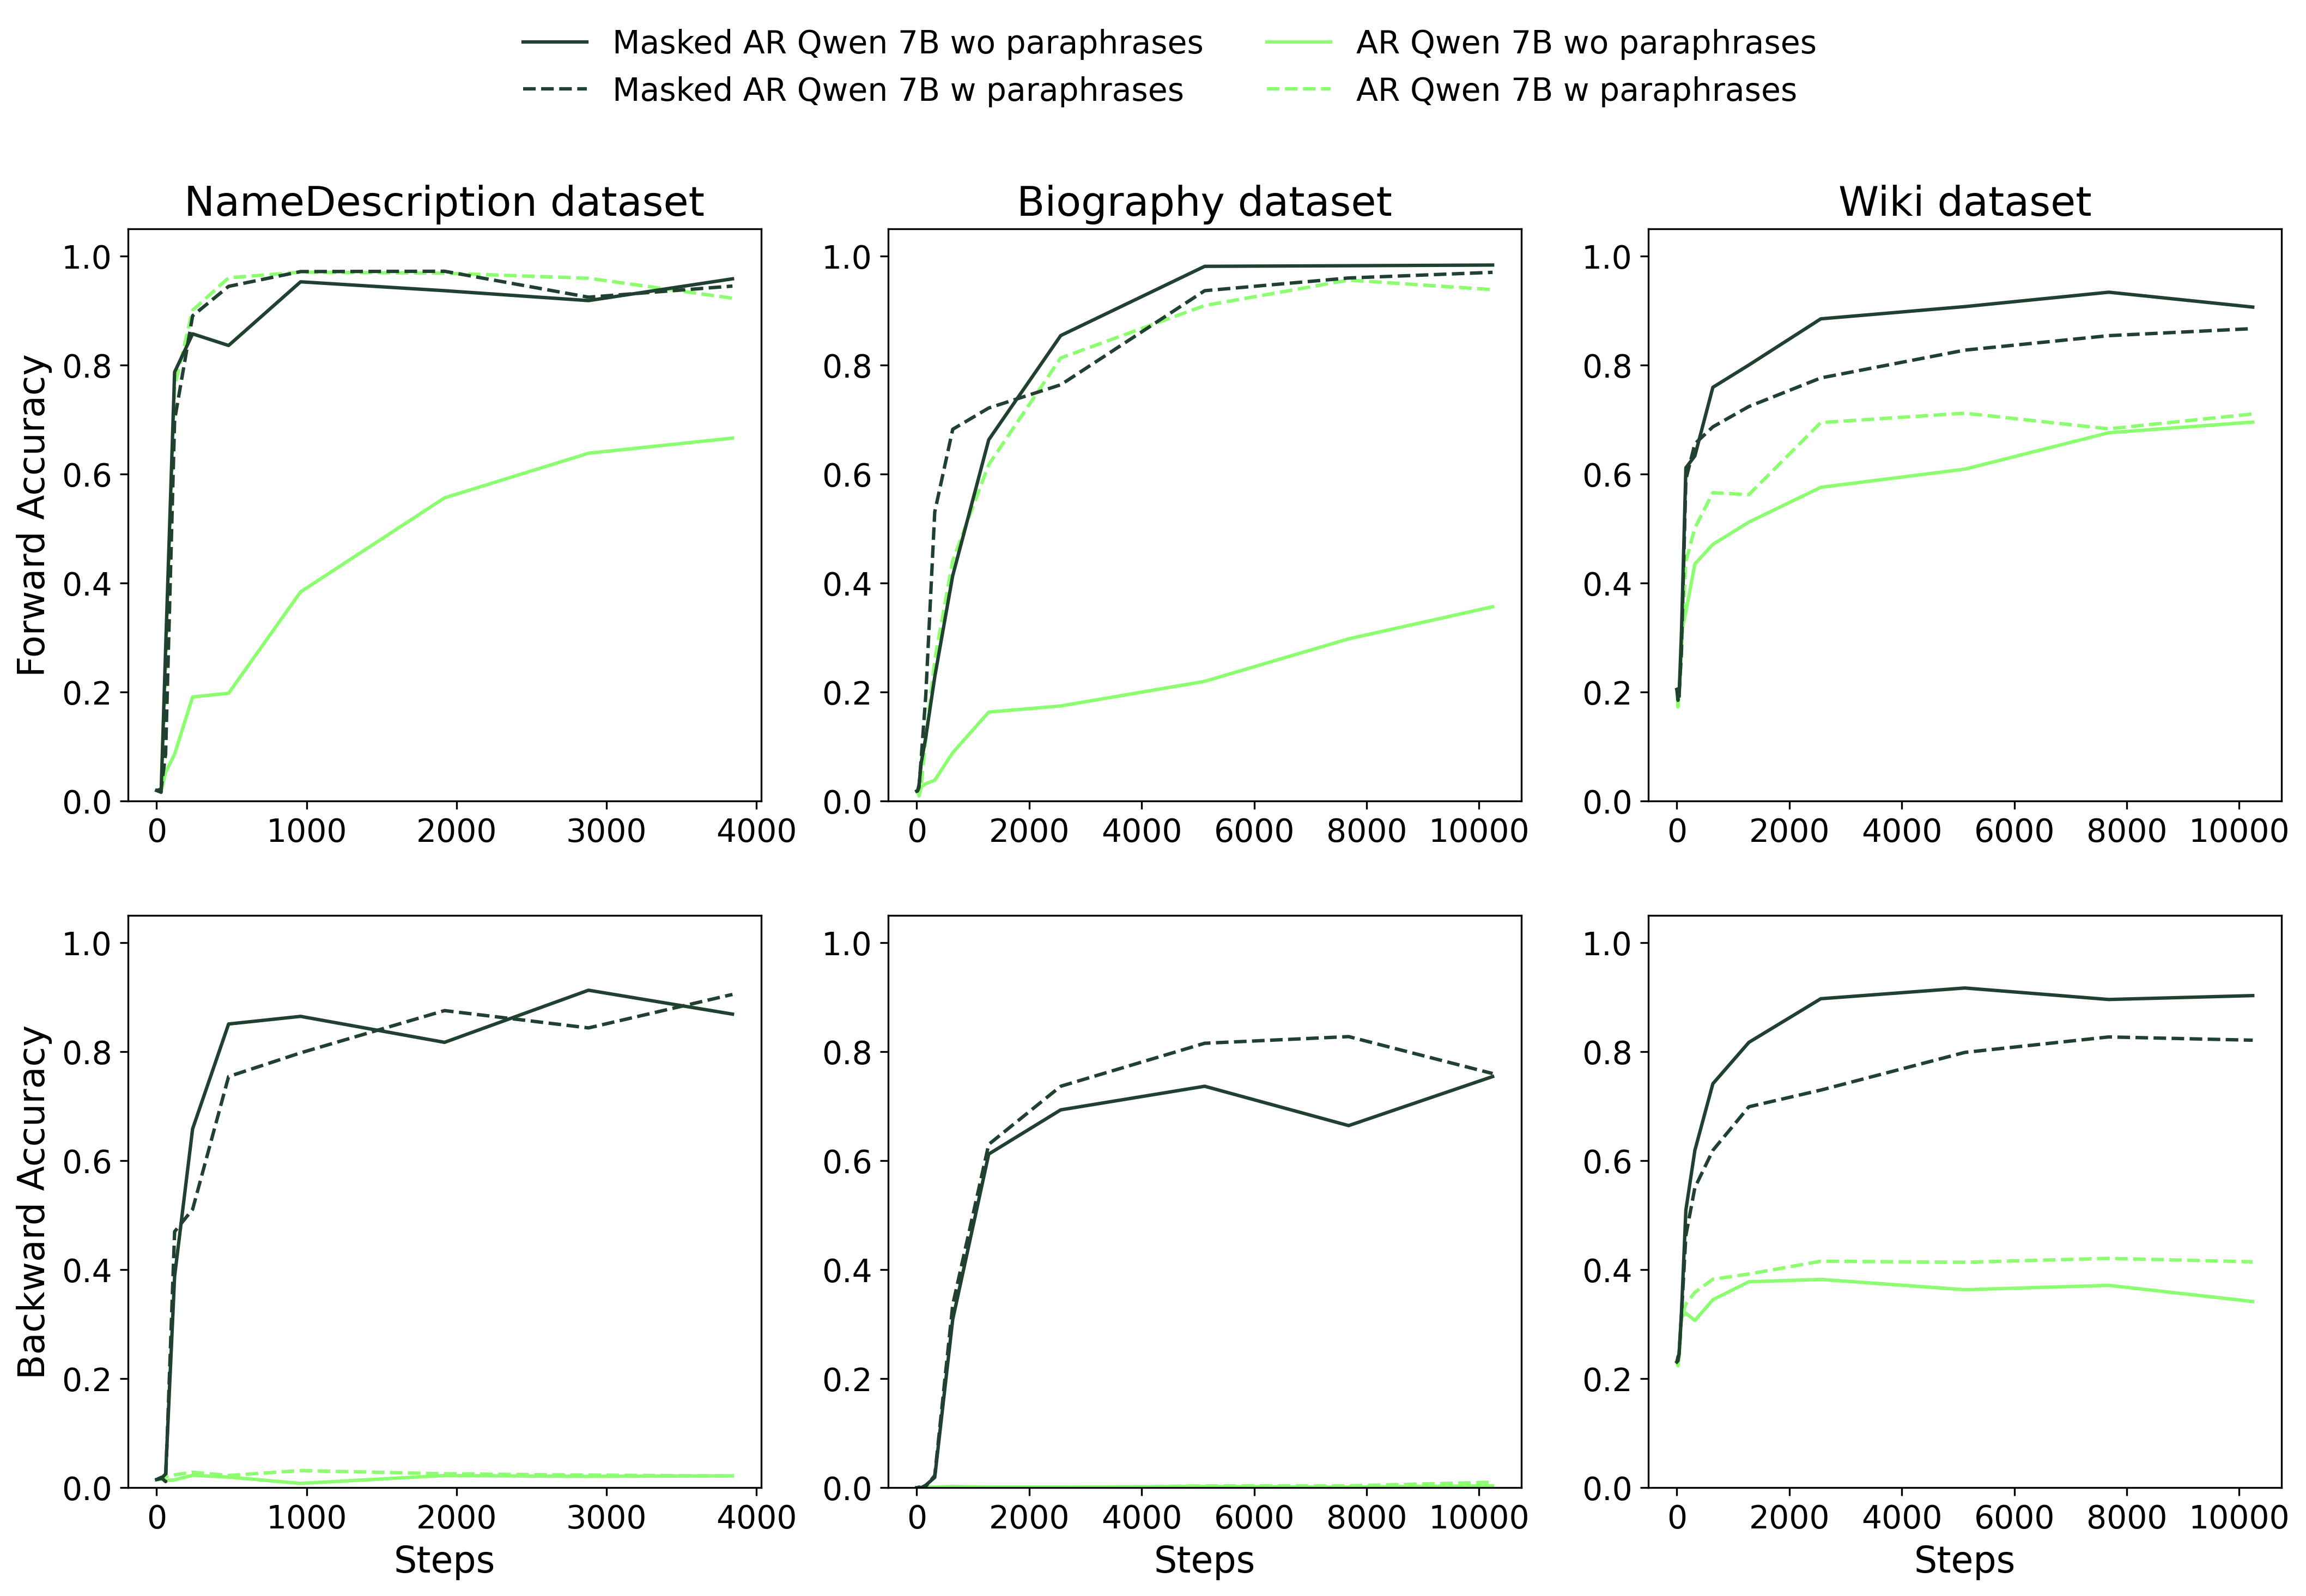
\includegraphics[width=0.75\linewidth]{figures/appendixc_fig07.png}
  \caption{Learning dynamics of Llama-3.2-3B-Instruct.}
  \label{fig:llama4b}
\end{figure}

\begin{figure}[htbp]
  \centering
  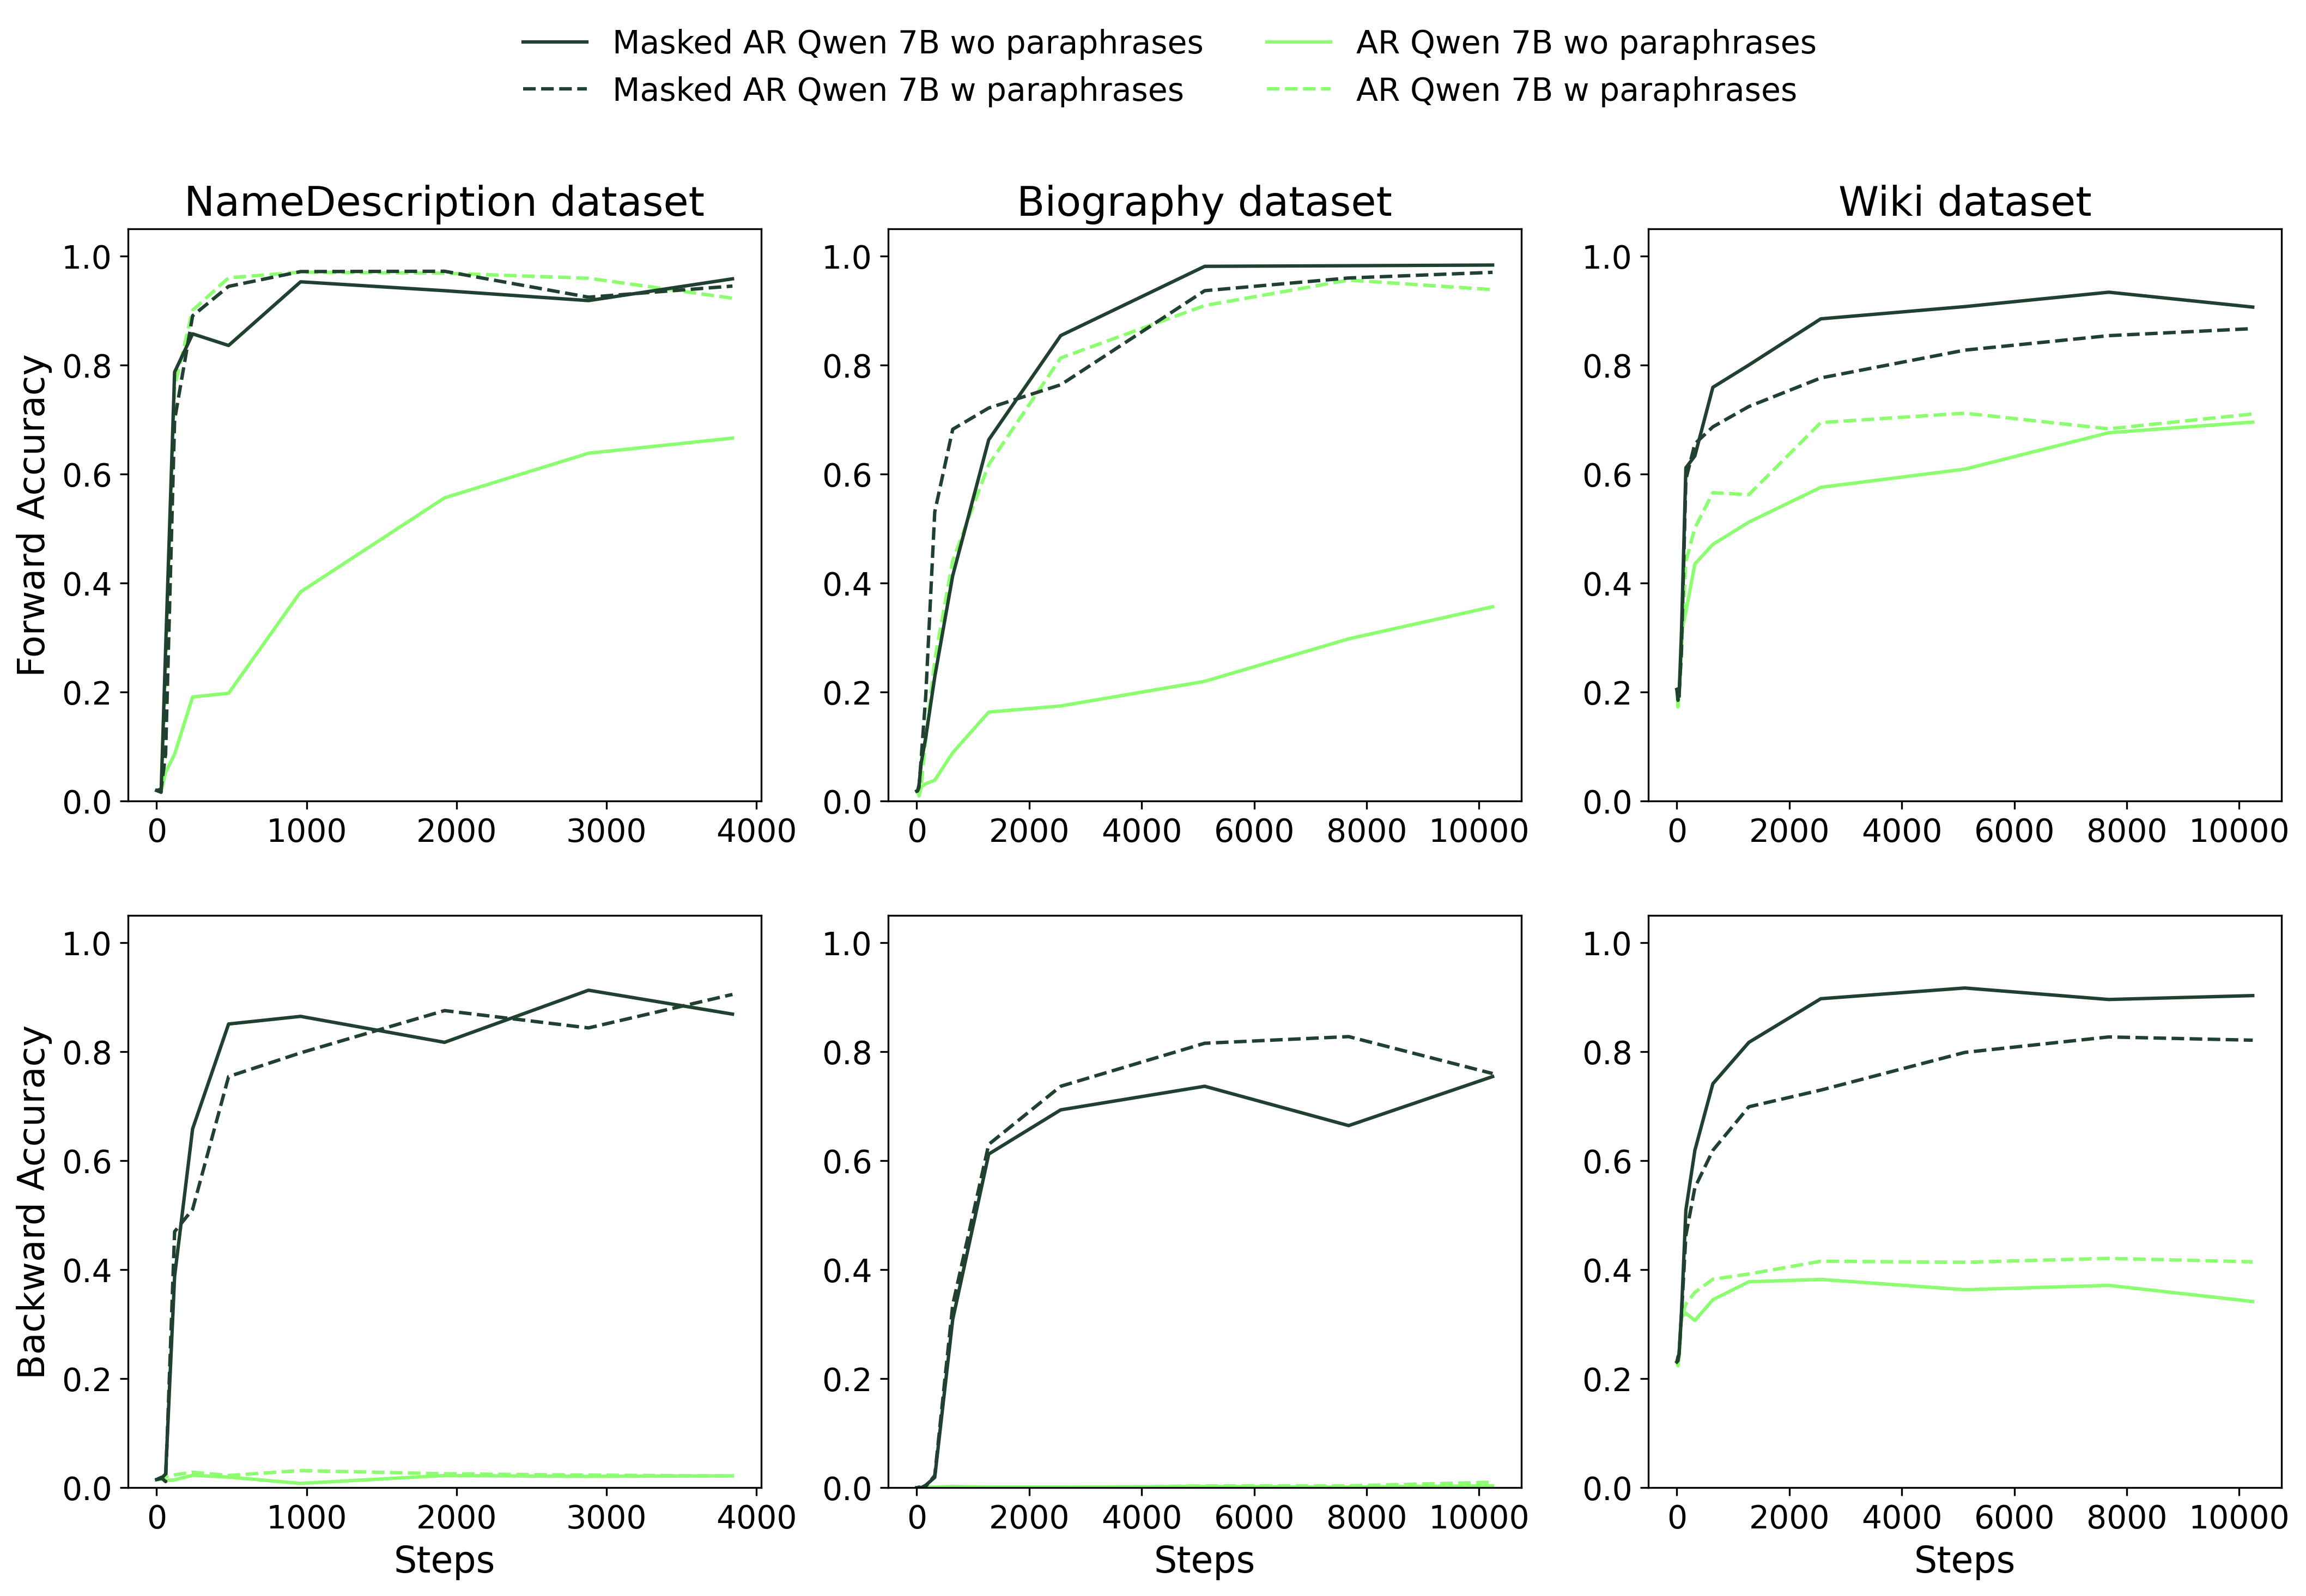
\includegraphics[width=0.75\linewidth]{figures/appendixc_fig08.png}
  \caption{Learning dynamics of Qwen/Qwen2.5-7B-Instruct.}
  \label{fig:qwen7b}
\end{figure}

\begin{figure}[htbp]
  \centering
  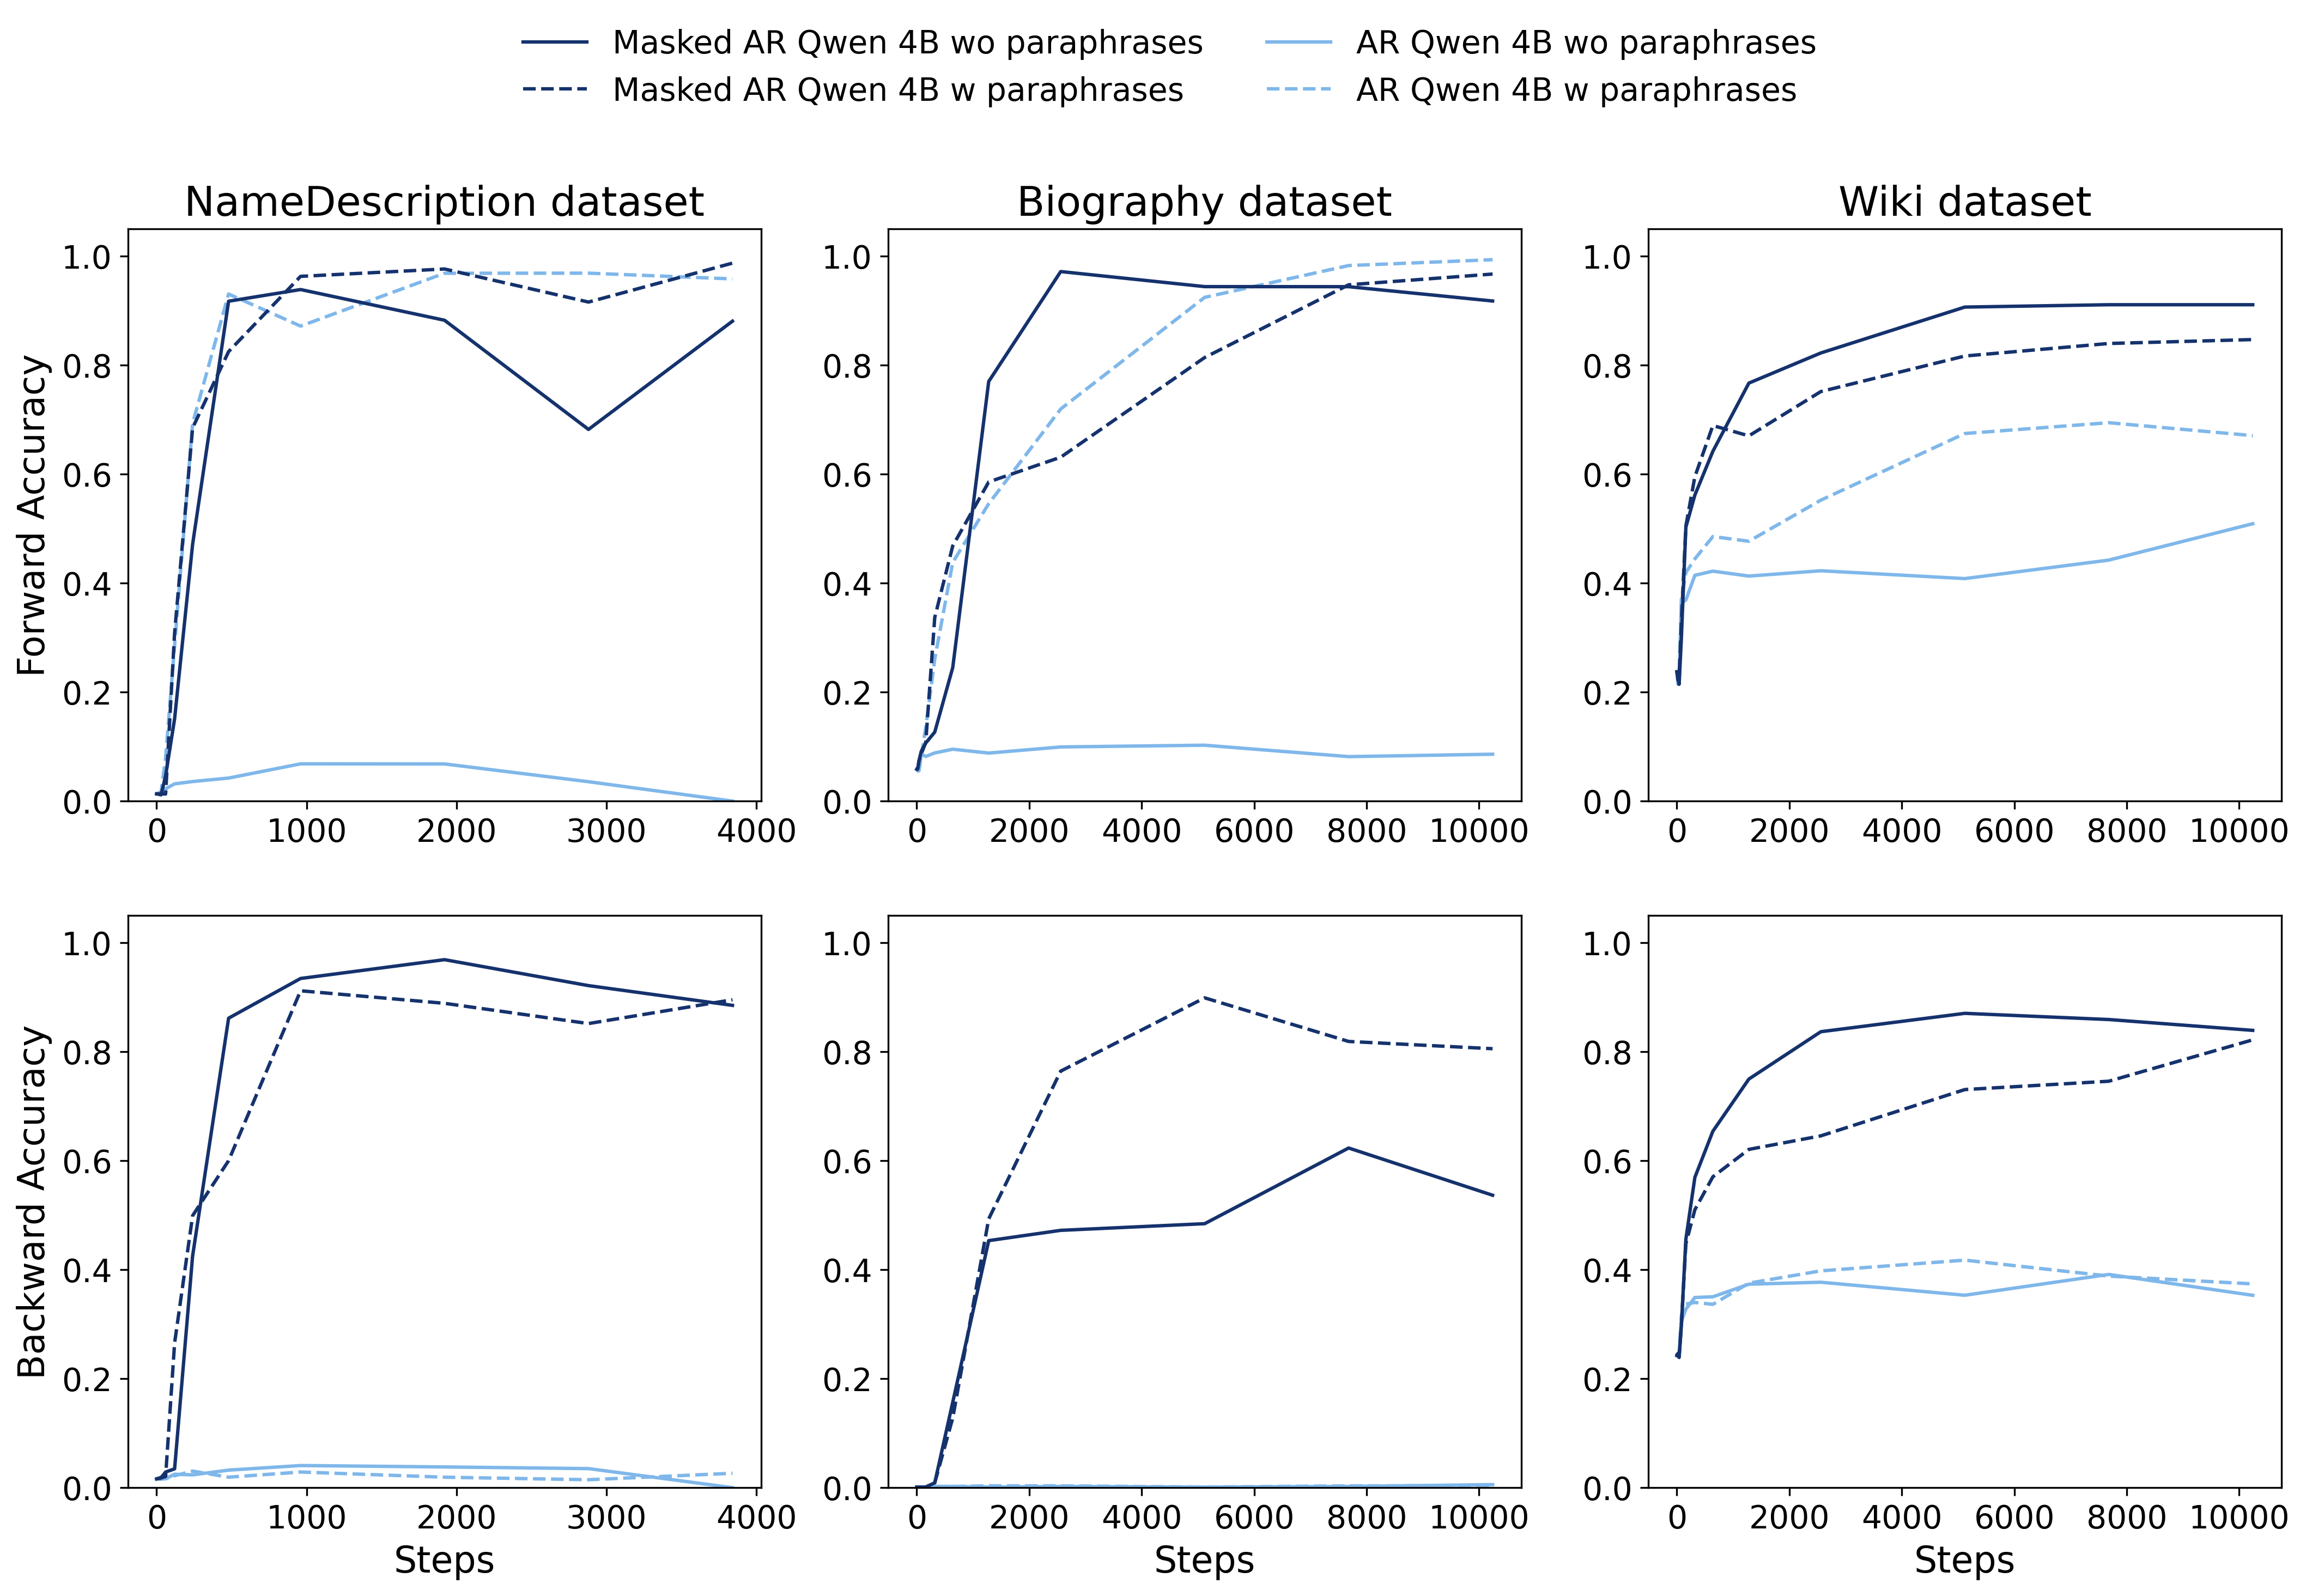
\includegraphics[width=0.75\linewidth]{figures/appendixc_fig09.png}
  \caption{Learning dynamics of Qwen/Qwen3-4B-Instruct-2507.}
  \label{fig:qwen3b}
\end{figure}

\begin{figure}[htbp]
  \centering
  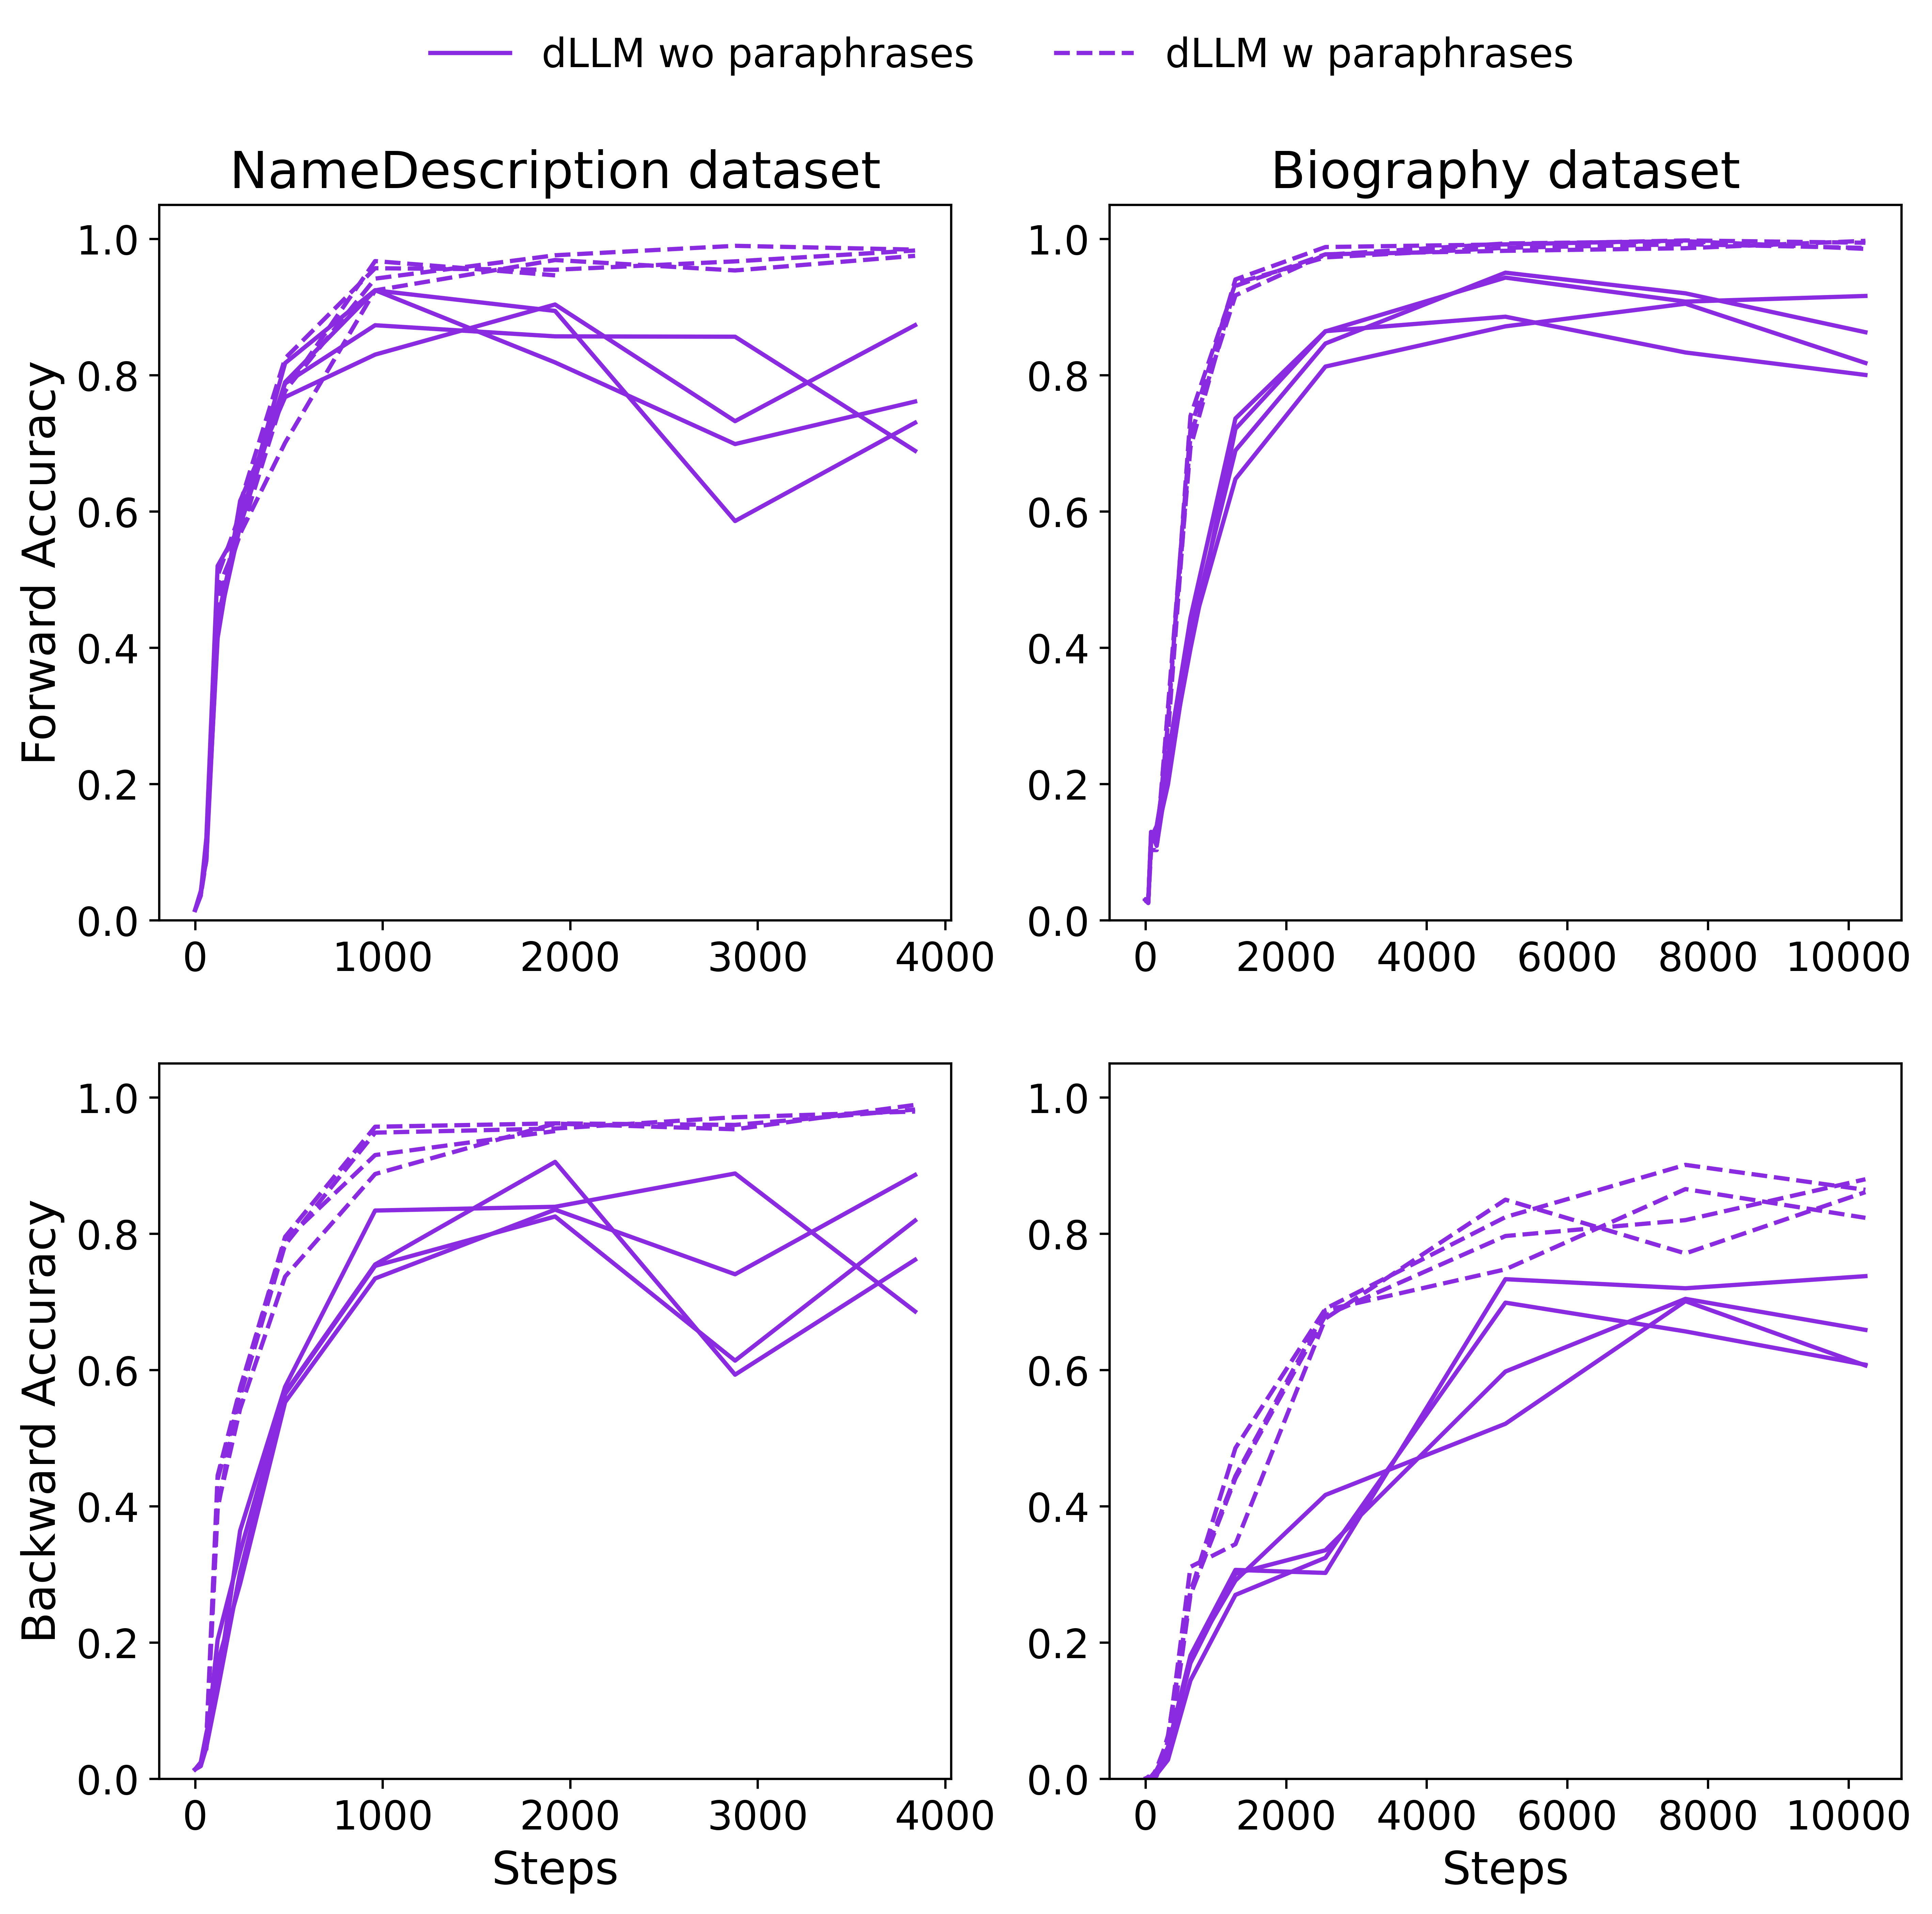
\includegraphics[width=0.6\linewidth]{figures/appendixc_fig10.png}
  \caption{Random seed effects in Llada. Random seed determines the sampling of mask ratio and masked tokens. Each line represent a random seed.}
  \label{fig:seed_dllm}
\end{figure}

\begin{figure}[htbp]
  \centering
  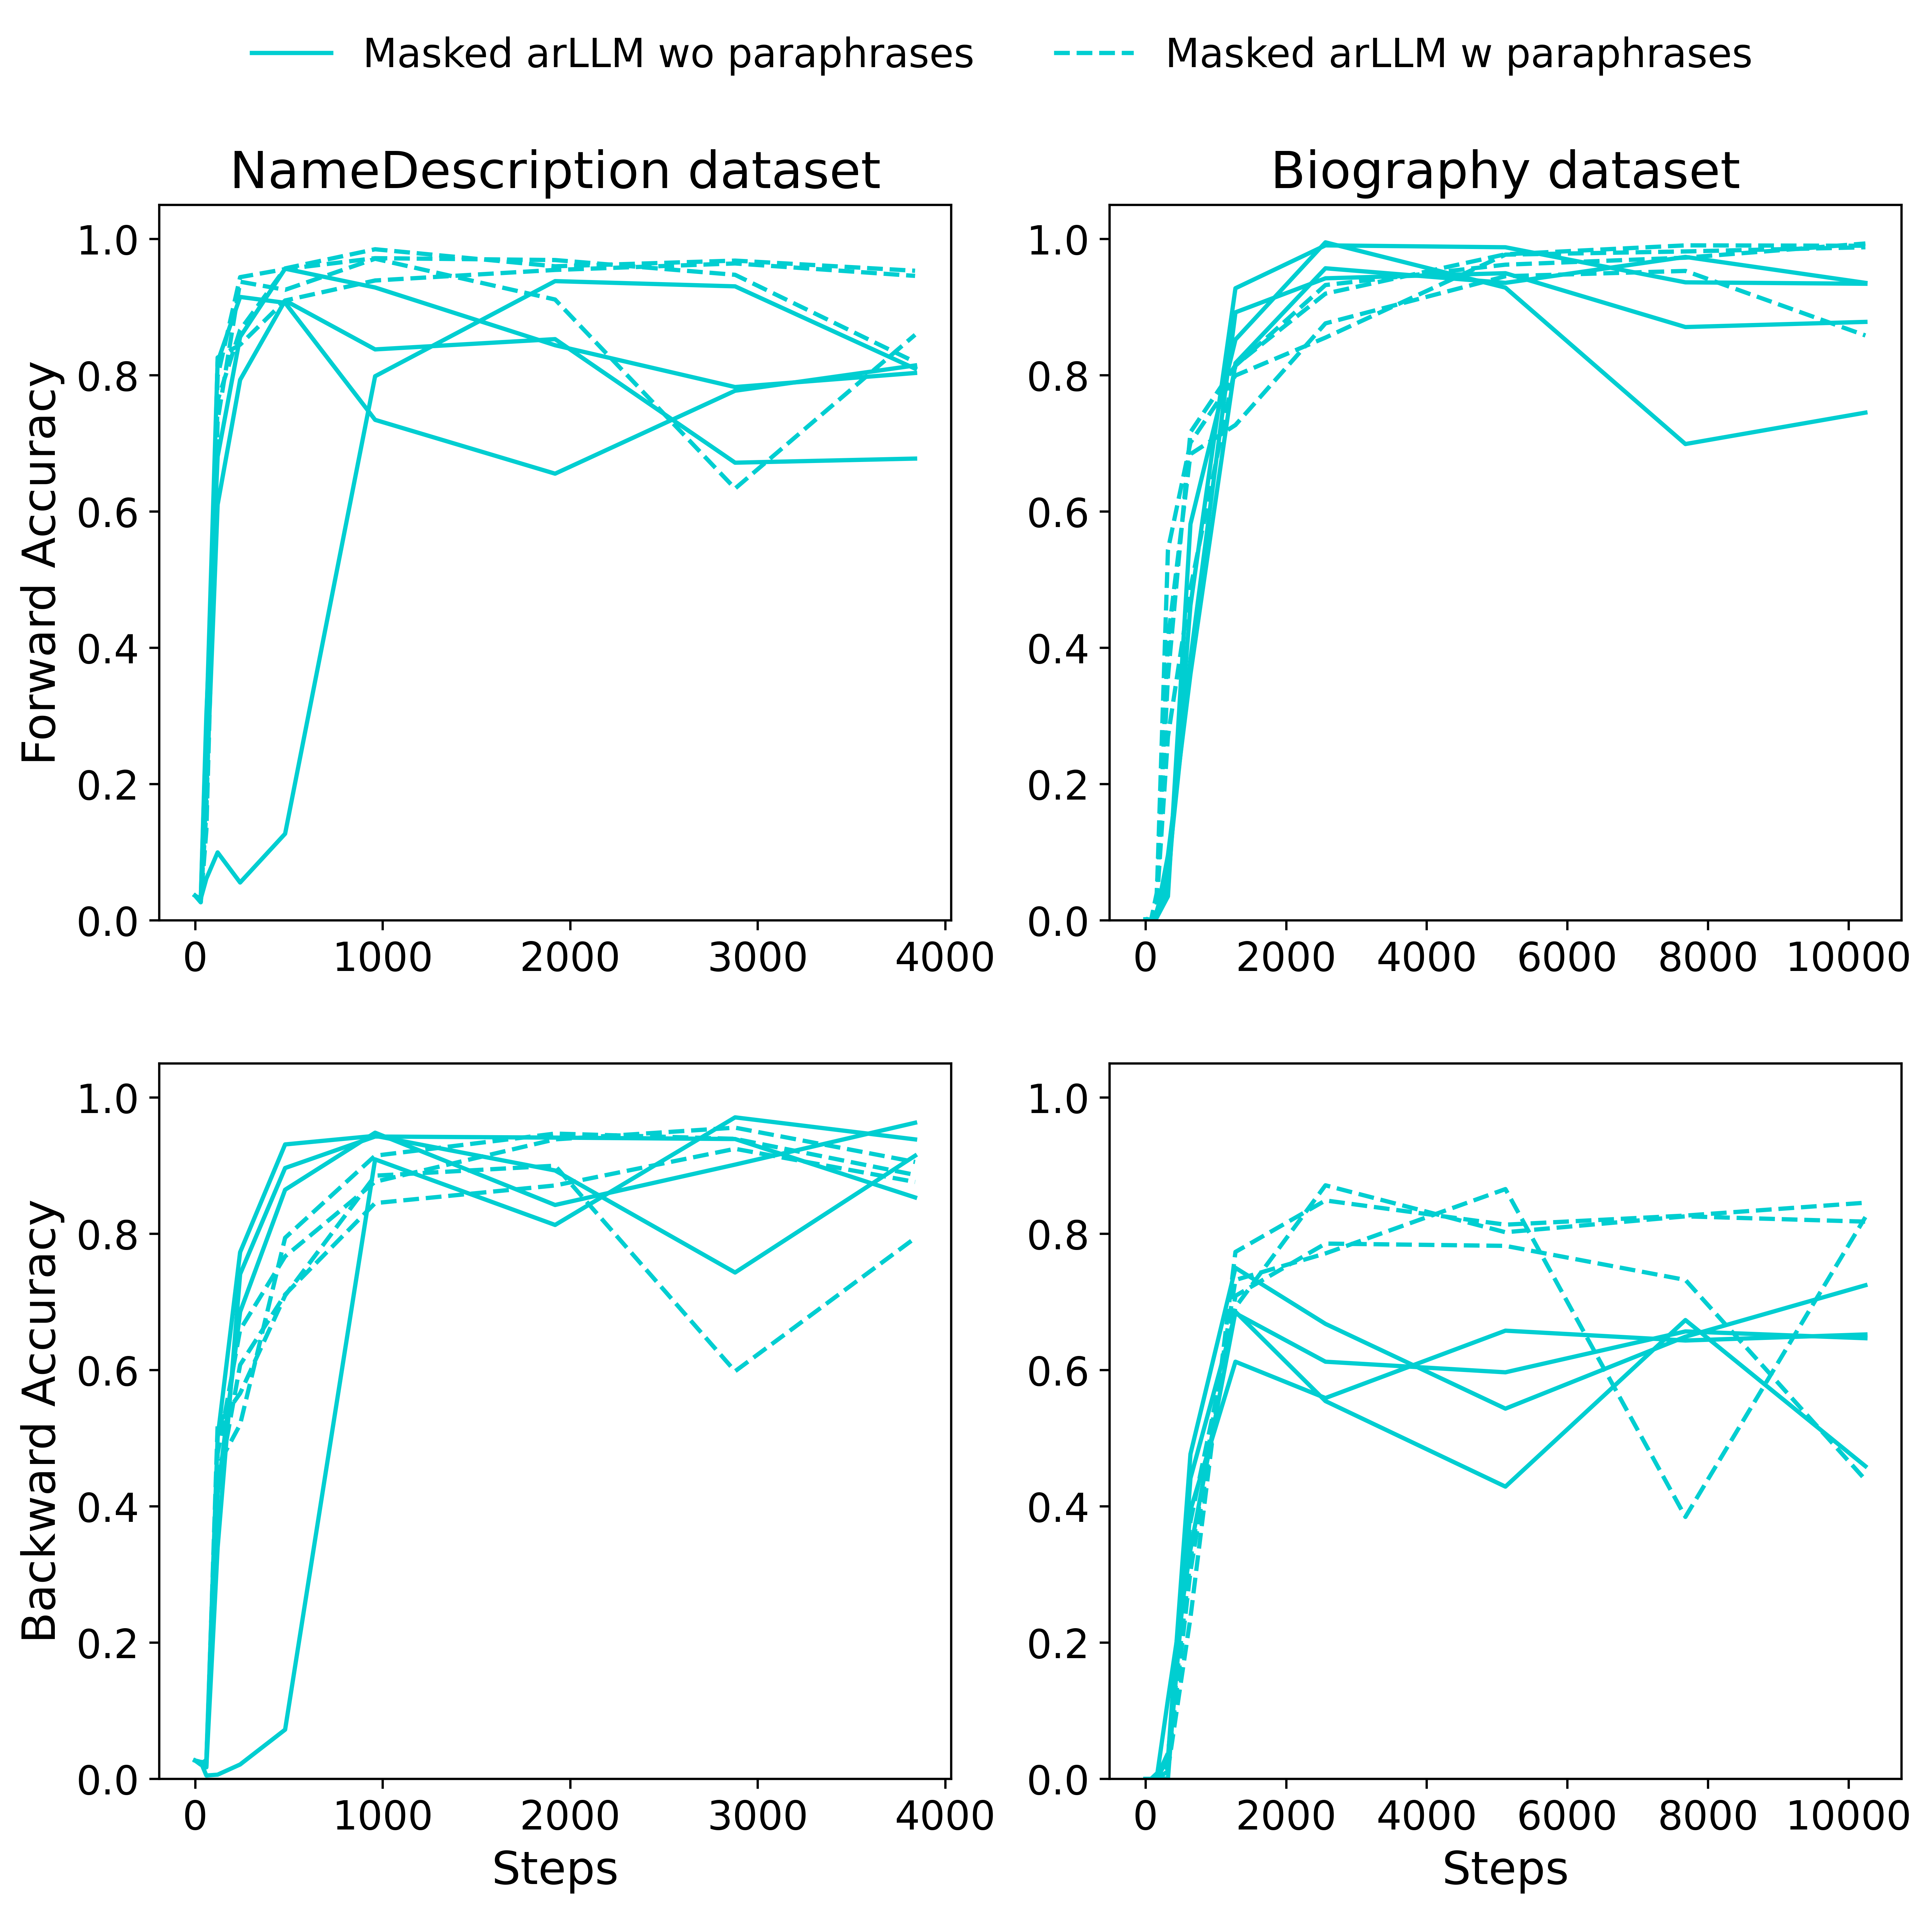
\includegraphics[width=0.6\linewidth]{figures/appendixc_fig11.png}
  \caption{Random seed effects in maksed Llama3.1 8B. Random seed determines the sampling of mask ratio and masked tokens. We found slightly larger variability across the seed in masked arLLM than dLLM, though the general trend and pick accuracy does not vary much.}
  \label{fig:seed_ar}
\end{figure}

\begin{figure}[htbp]
  \centering
  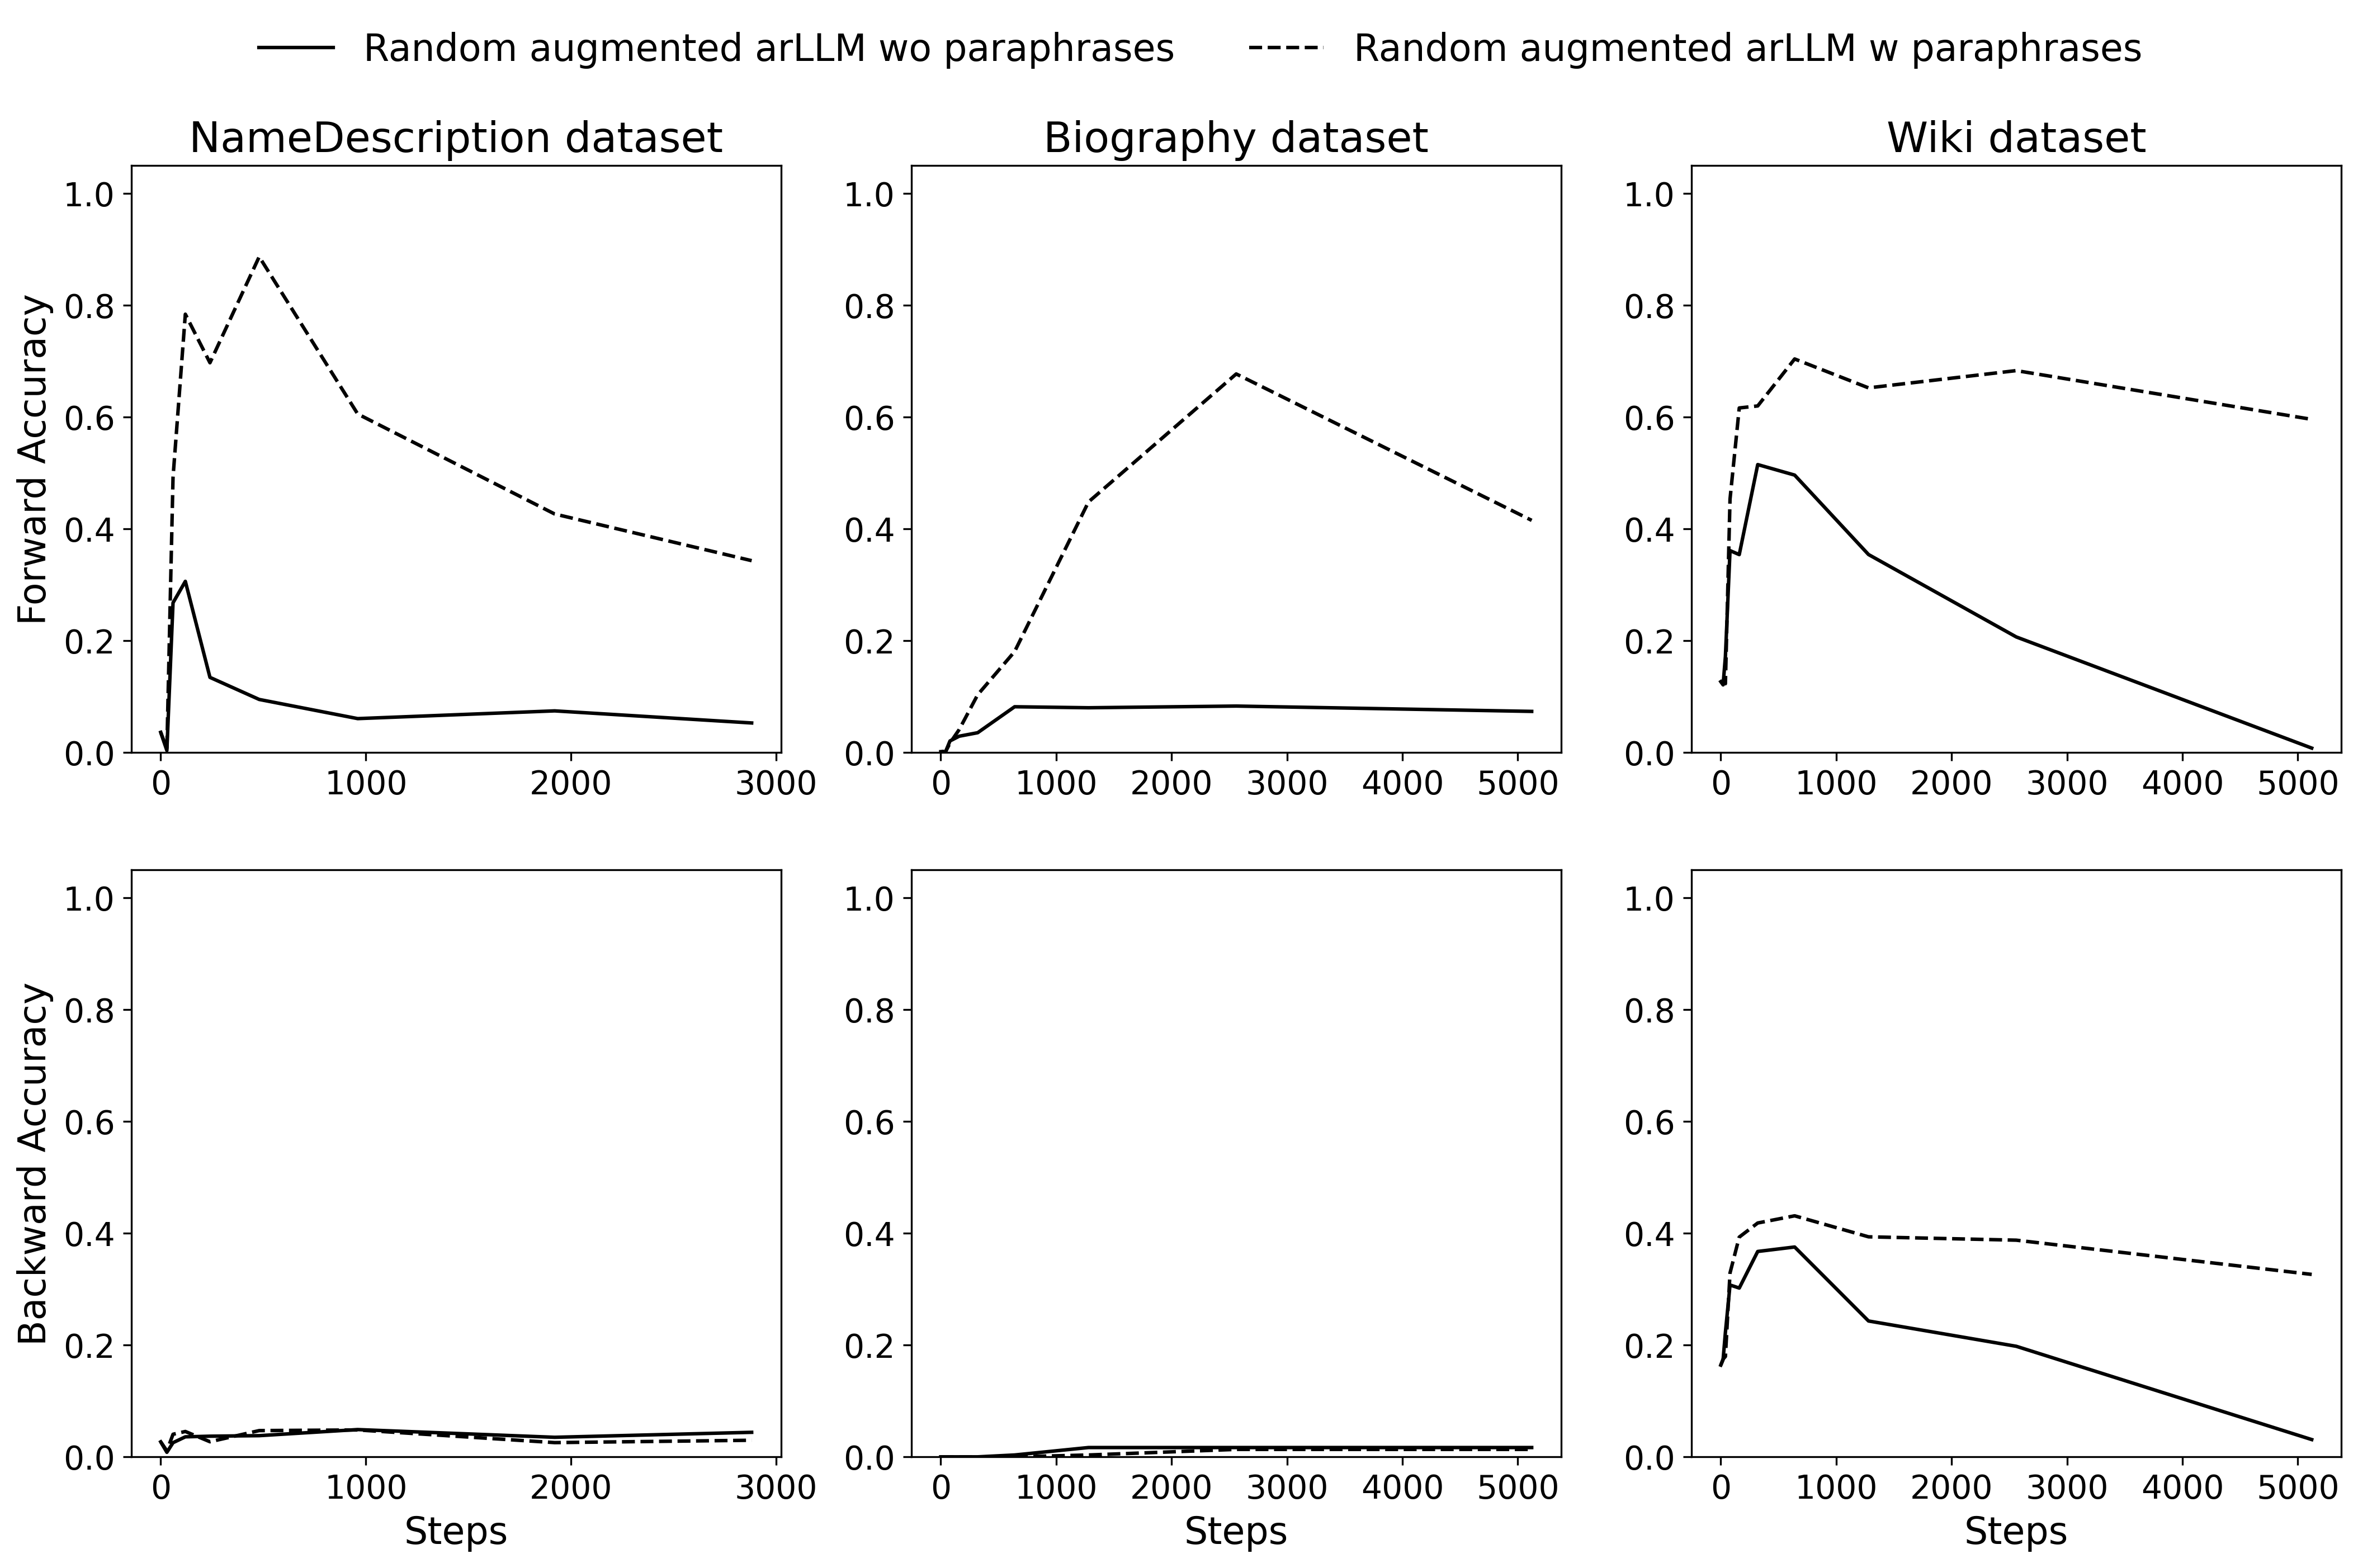
\includegraphics[width=0.75\linewidth]{figures/appendixc_fig12.png}
  \caption{To verify the advantage of masked fine-tuning of arLLMs is not simply due ``data augmentation'' (i.e. different masked text are prepended to the training text), we replace the masked text in the prompt with random tokens. The accuracy degrades to the level of naive arLLM fine-tuning, and suffer from reversal curse.}
  \label{fig:random_augmentation}
\end{figure}

\begin{table}[htbp]
\centering
\caption{To compare the rate of convergence, we fit the accuracy curve as a function of training steps to $A(1-e^{-kx})$. ``$A$'' is the accuracy at convergence; $k$ is the rate of convergence (unit $1/step$).}
\label{tab:convergence}
\scriptsize
\setlength{\tabcolsep}{4pt}
\renewcommand{\arraystretch}{1.15}
\resizebox{\textwidth}{!}{\begin{tabular}{*{13}{c}}
\toprule
& \multicolumn{4}{c}{NameDescription} & \multicolumn{4}{c}{Biography} & \multicolumn{4}{c}{Wiki} \\
\cmidrule(lr){2-5}\cmidrule(lr){6-9}\cmidrule(lr){10-13}
 & \multicolumn{2}{c}{Forward} & \multicolumn{2}{c}{Backward} & \multicolumn{2}{c}{Forward} & \multicolumn{2}{c}{Backward} & \multicolumn{2}{c}{Forward} & \multicolumn{2}{c}{Backward} \\
& A & k & A & k & A & k & A & k & A & k & A & k \\
\midrule
AR w paraphrases        & 0.862 & 0.0093 & 0.026 & 0.0411 & 0.960 & 0.0008 & 0.002 & 0.0006 & 0.630 & 0.0069 & 0.361 & 0.0130 \\
AR wo paraphrases       & 0.069 & 0.0502 & 0.014 & 0.5562 & 0.062 & 0.0034 & 0.001 & 0.0007 & 0.241 & 0.0350 & 0.182 & 0.1337 \\
dLLM w paraphrases      & 0.968 & 0.0038 & 0.967 & 0.0035 & 1.006 & 0.0015 & 0.864 & 0.0005 & 0.878 & 0.0049 & 0.734 & 0.0073 \\
dLLM wo paraphrases     & 0.819 & 0.0052 & 0.798 & 0.0024 & 0.777 & 0.0005 & 0.783 & 0.0001 & 0.897 & 0.0052 & 0.704 & 0.0081 \\
Masked arLLM w paraphrases & 0.944 & 0.0082 & 0.883 & 0.0042 & 0.961 & 0.0014 & 0.786 & 0.0010 & 0.759 & 0.0024 & 0.686 & 0.0018 \\
Masked arLLM wo paraphrases& 0.799 & 0.0068 & 0.911 & 0.0032 & 0.957 & 0.0009 & 0.617 & 0.0012 & 0.933 & 0.0032 & 0.883 & 0.0029 \\
\bottomrule
\end{tabular}}

\end{table}

\subsection{Masked SFT training configs}

In Section \ref{sec:sft}, we proposed a Masked SFT method that turns any SFT prompt-response sequence into a demasking task. Specifically, the constructed demasking task sequence contains the question and masked answer in the user prompt, and full answer in the assistant response. For example, a data entry in the GSM8K dataset is: \textbf{Question}:
Joy can read 8 pages of a book in 20 minutes. How many hours will it take her to read 120 pages? \textbf{Answer}: In one hour, there are 3 sets of 20 minutes. So, Joy can read 8 x 3 = <<8*3=24>>24 pages in an hour. It will take her 120/24 = <<120/24=5>>5 hours to read 120 pages. 5. After generating a random mask, the constructed masked SFT sequence is: 

\begin{center}
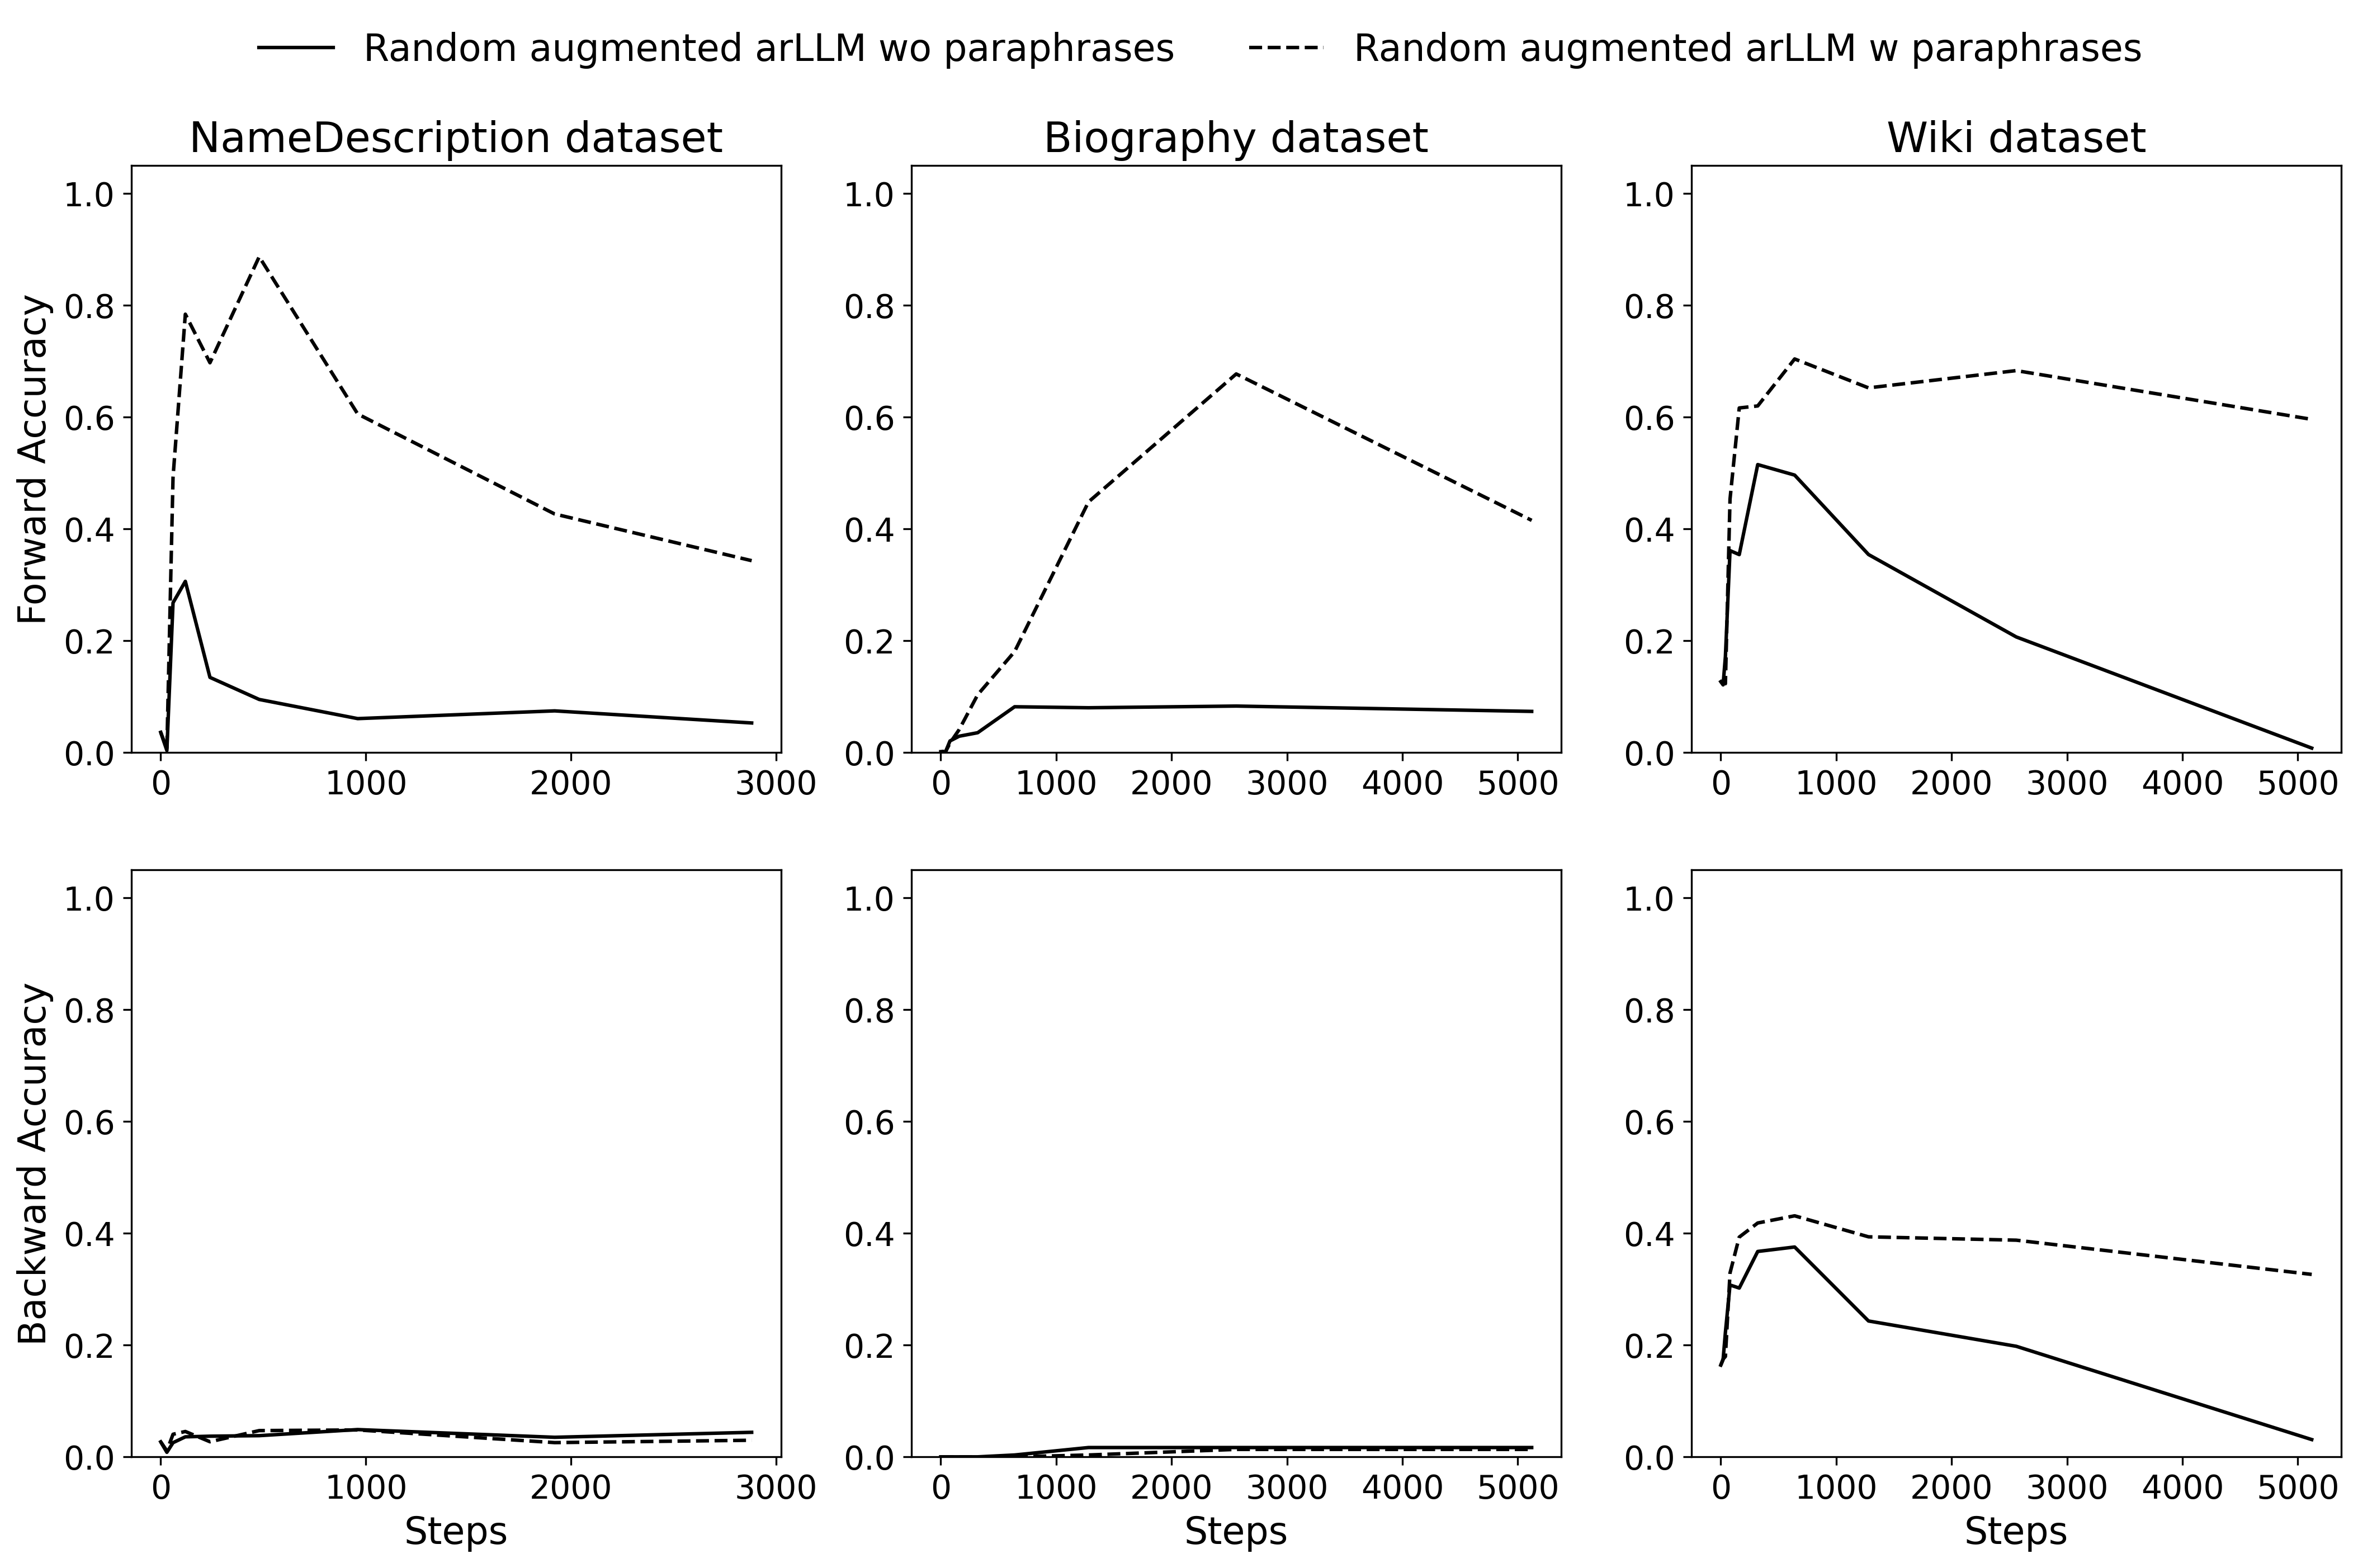
\includegraphics[width=0.95\linewidth]{figures/appendixc_fig12.png}
\end{center}



We compute loss only on the highlighted tokens. More specifically, in Eq. \ref{eq:2}, $m_i$ is set to $1$ when the $i$th token is in the assistant response and its corresponding token in the user prompt is masked.

We choose to use the GSM8K and MATH datasets for testing the SFT performance on Llama-3.2-3B-Instruct and Qwen/Qwen3-4B-Instruct-2507. For the MATH dataset, we use the default subset from huggingface DigitalLearningGmbH/MATH-lighteval. We further filter out the training samples whose token lengths (question + answer) are longer than 512. When evaluating the resulting models, we use the evaluation framework \texttt{LM Evaluation Harness} and the default tasks \texttt{gsm8k} and \texttt{hendrycks\_math} (\cite{eval-harness}). Specifically, we choose to use 0-shot and pass@1 with a maximum generation length of 256 at a temperature of 0. For GSM8K we report the accuracy using exact match with \texttt{LM Evaluation Harness}'s flexible extraction. For MATH we report the accuracy using exact match with \texttt{math-verify} extraction (\cite{Kydlicek_Math-Verify_Math_Verification}). Both extraction methods are chosen to maximize alignment with human examination.  

Most of the training configurations are the same as those in the main experiments, except for the following changes. The batch size is 32 for the GSM8K dataset, and 16 for the MATH dataset. We set maximum training epoch to 7, and reported the best testing accuracy across the training. Optimal learning rate is found for each model and dataset pair and shown in the following figures (Appendix Figure \ref{apx:llama3b_gsm8k}-\ref{apx:qwen4b_math}). 


\begin{figure}[htbp]
  \centering
  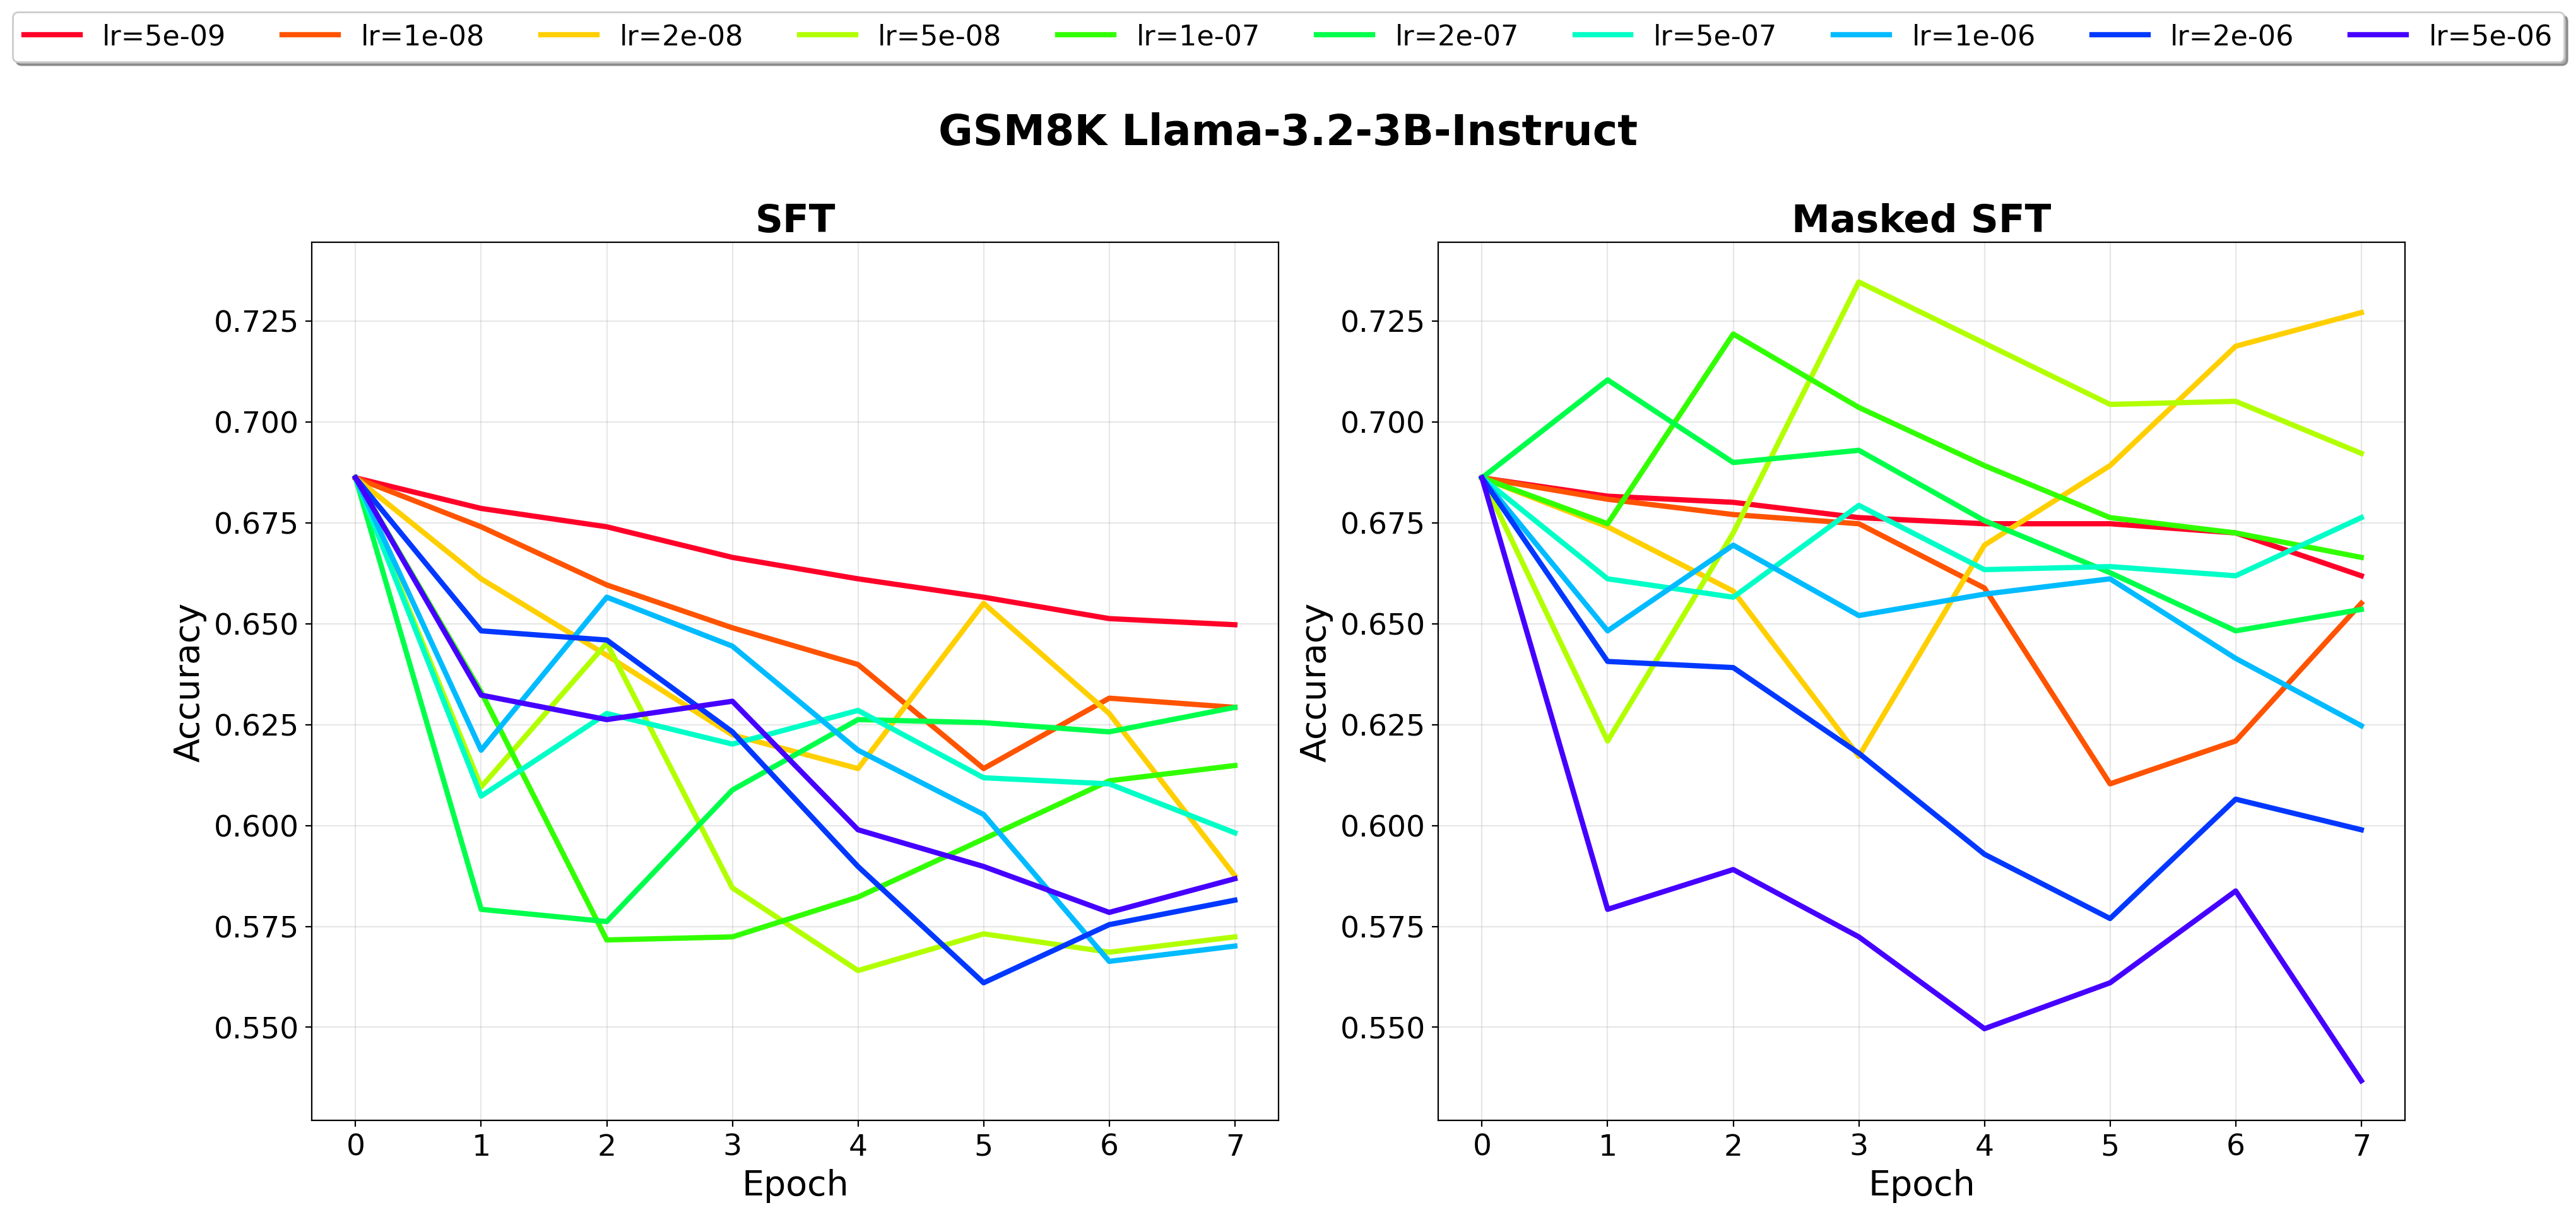
\includegraphics[width=0.7\linewidth]{figures/appendixc_fig14.png}
  \caption{Learning rate and epoch sweep of Llama-3.2-3B-Instruct on GSM8K dataset.}
  \label{apx:llama3b_gsm8k}
\end{figure}

\begin{figure}[htbp]
  \centering
  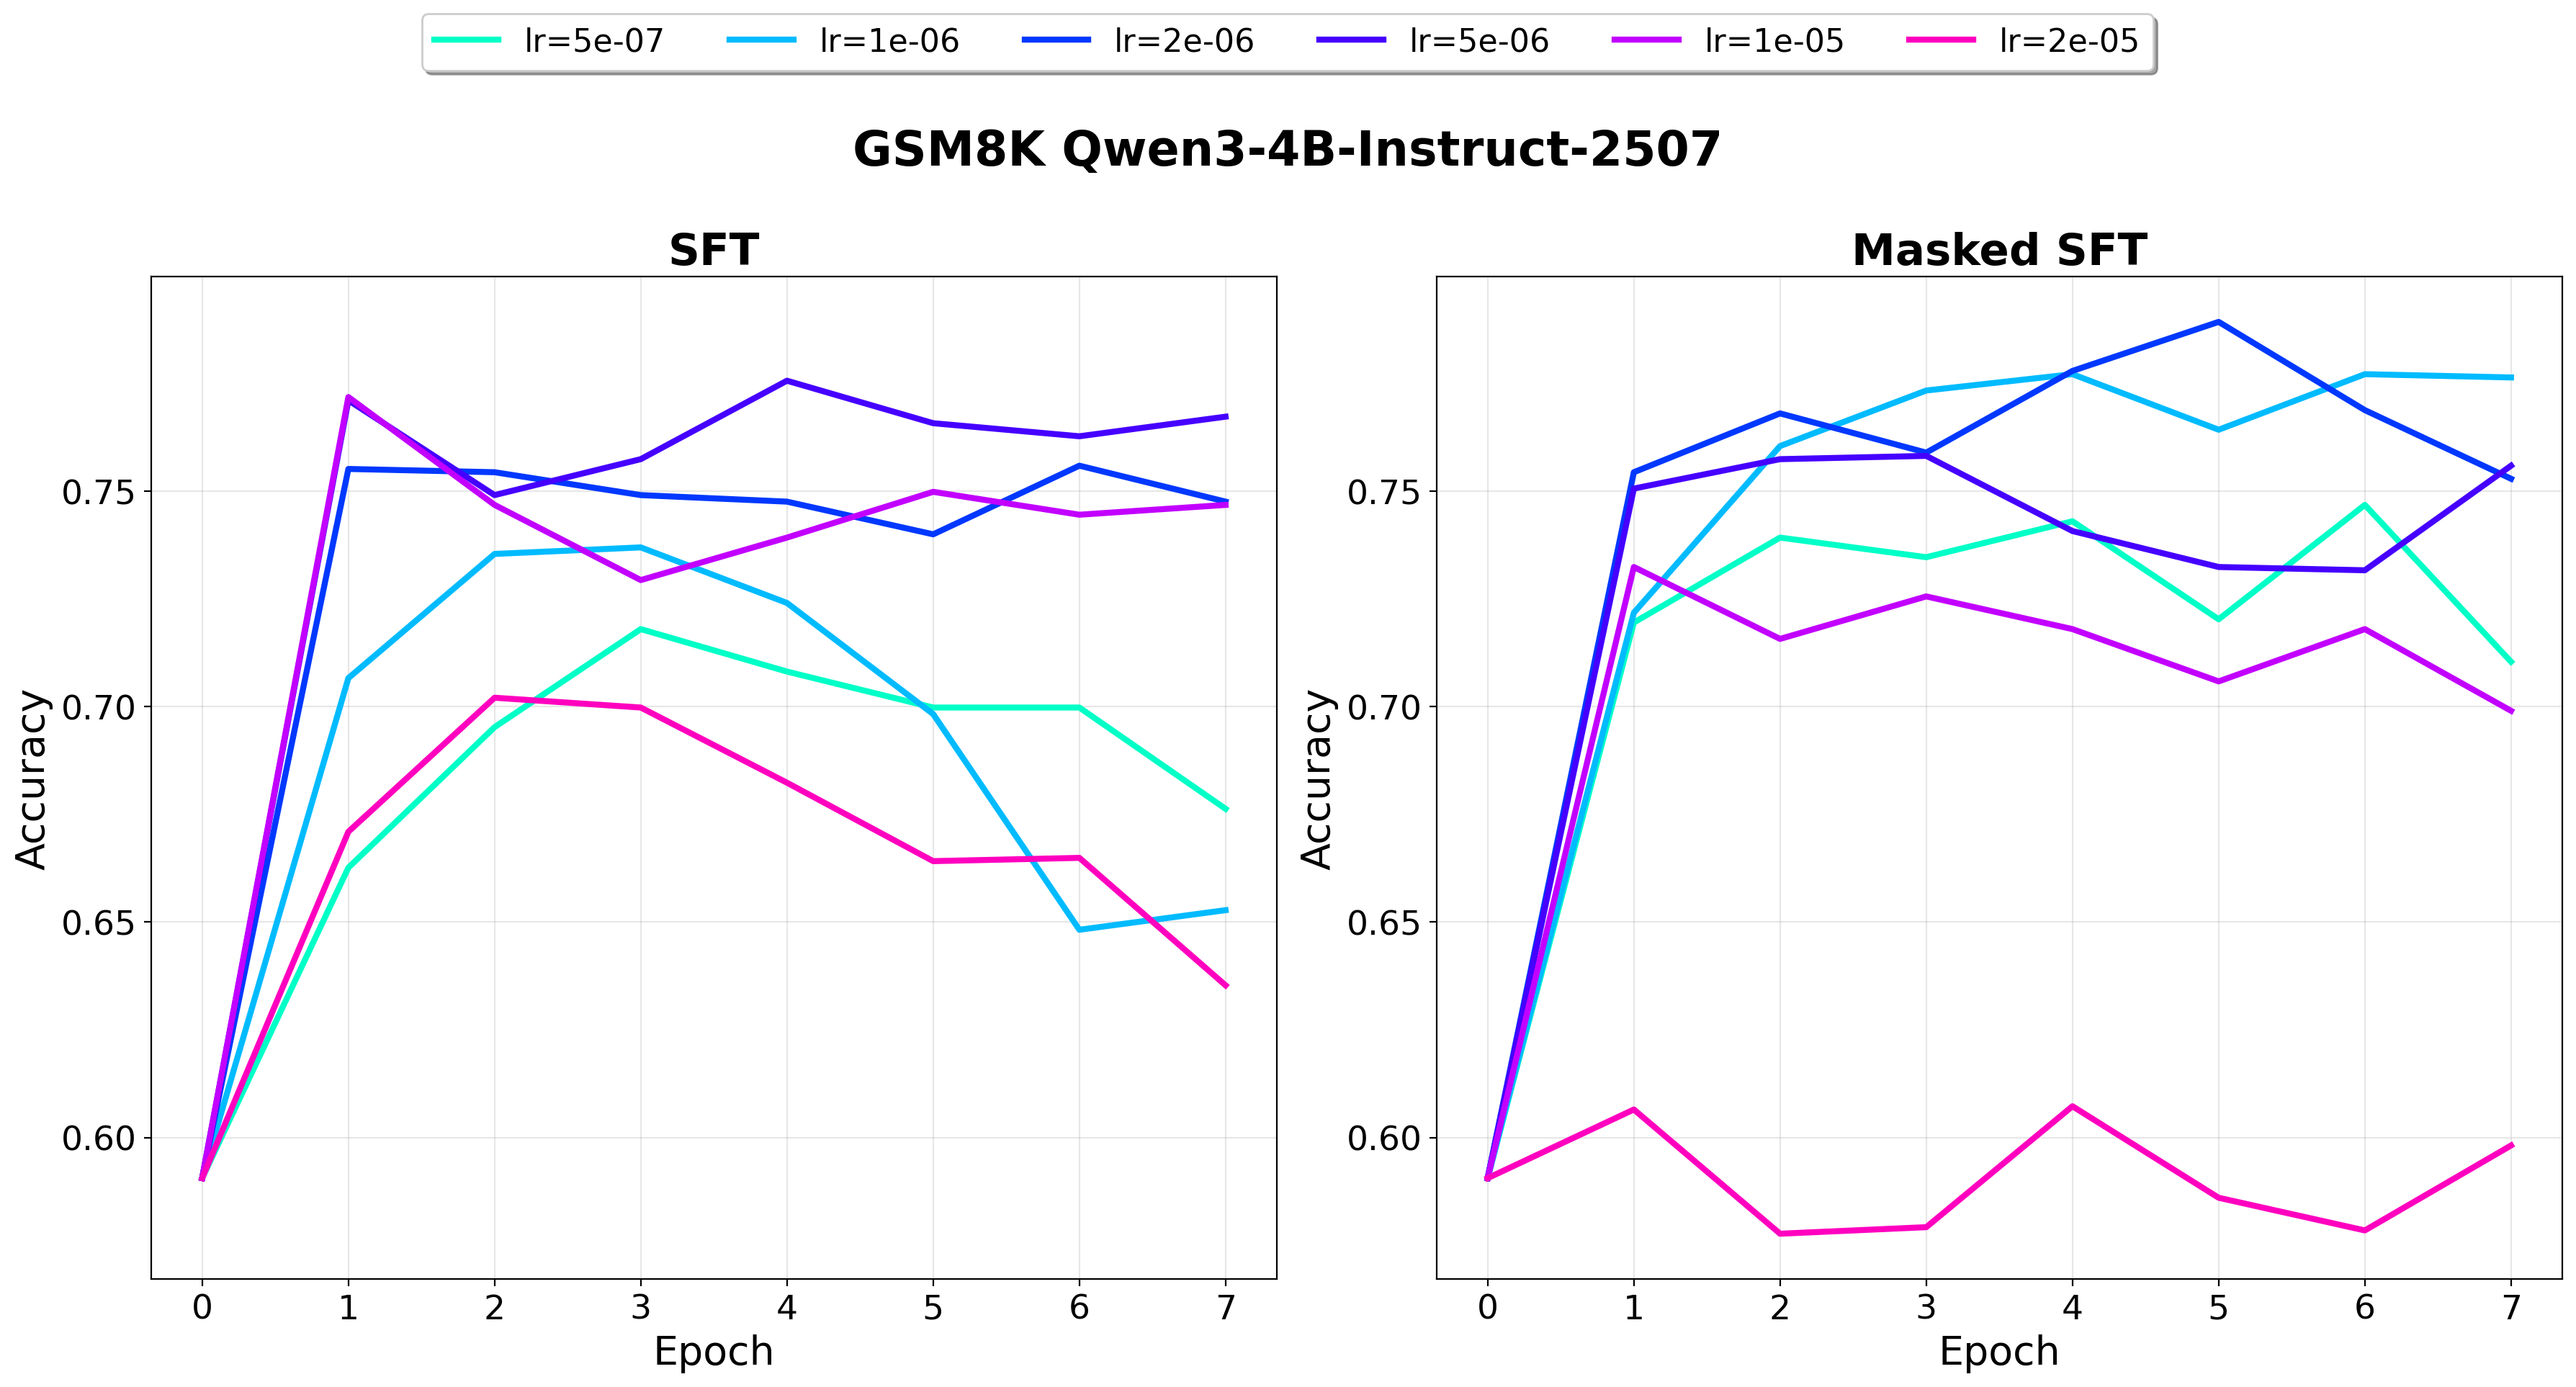
\includegraphics[width=0.7\linewidth]{figures/appendixc_fig15.png}
  \caption{Learning rate and epoch sweep of Qwen3-4B-Instruct-2507 on GSM8K dataset.}
\end{figure}

\begin{figure}[htbp]
  \centering
  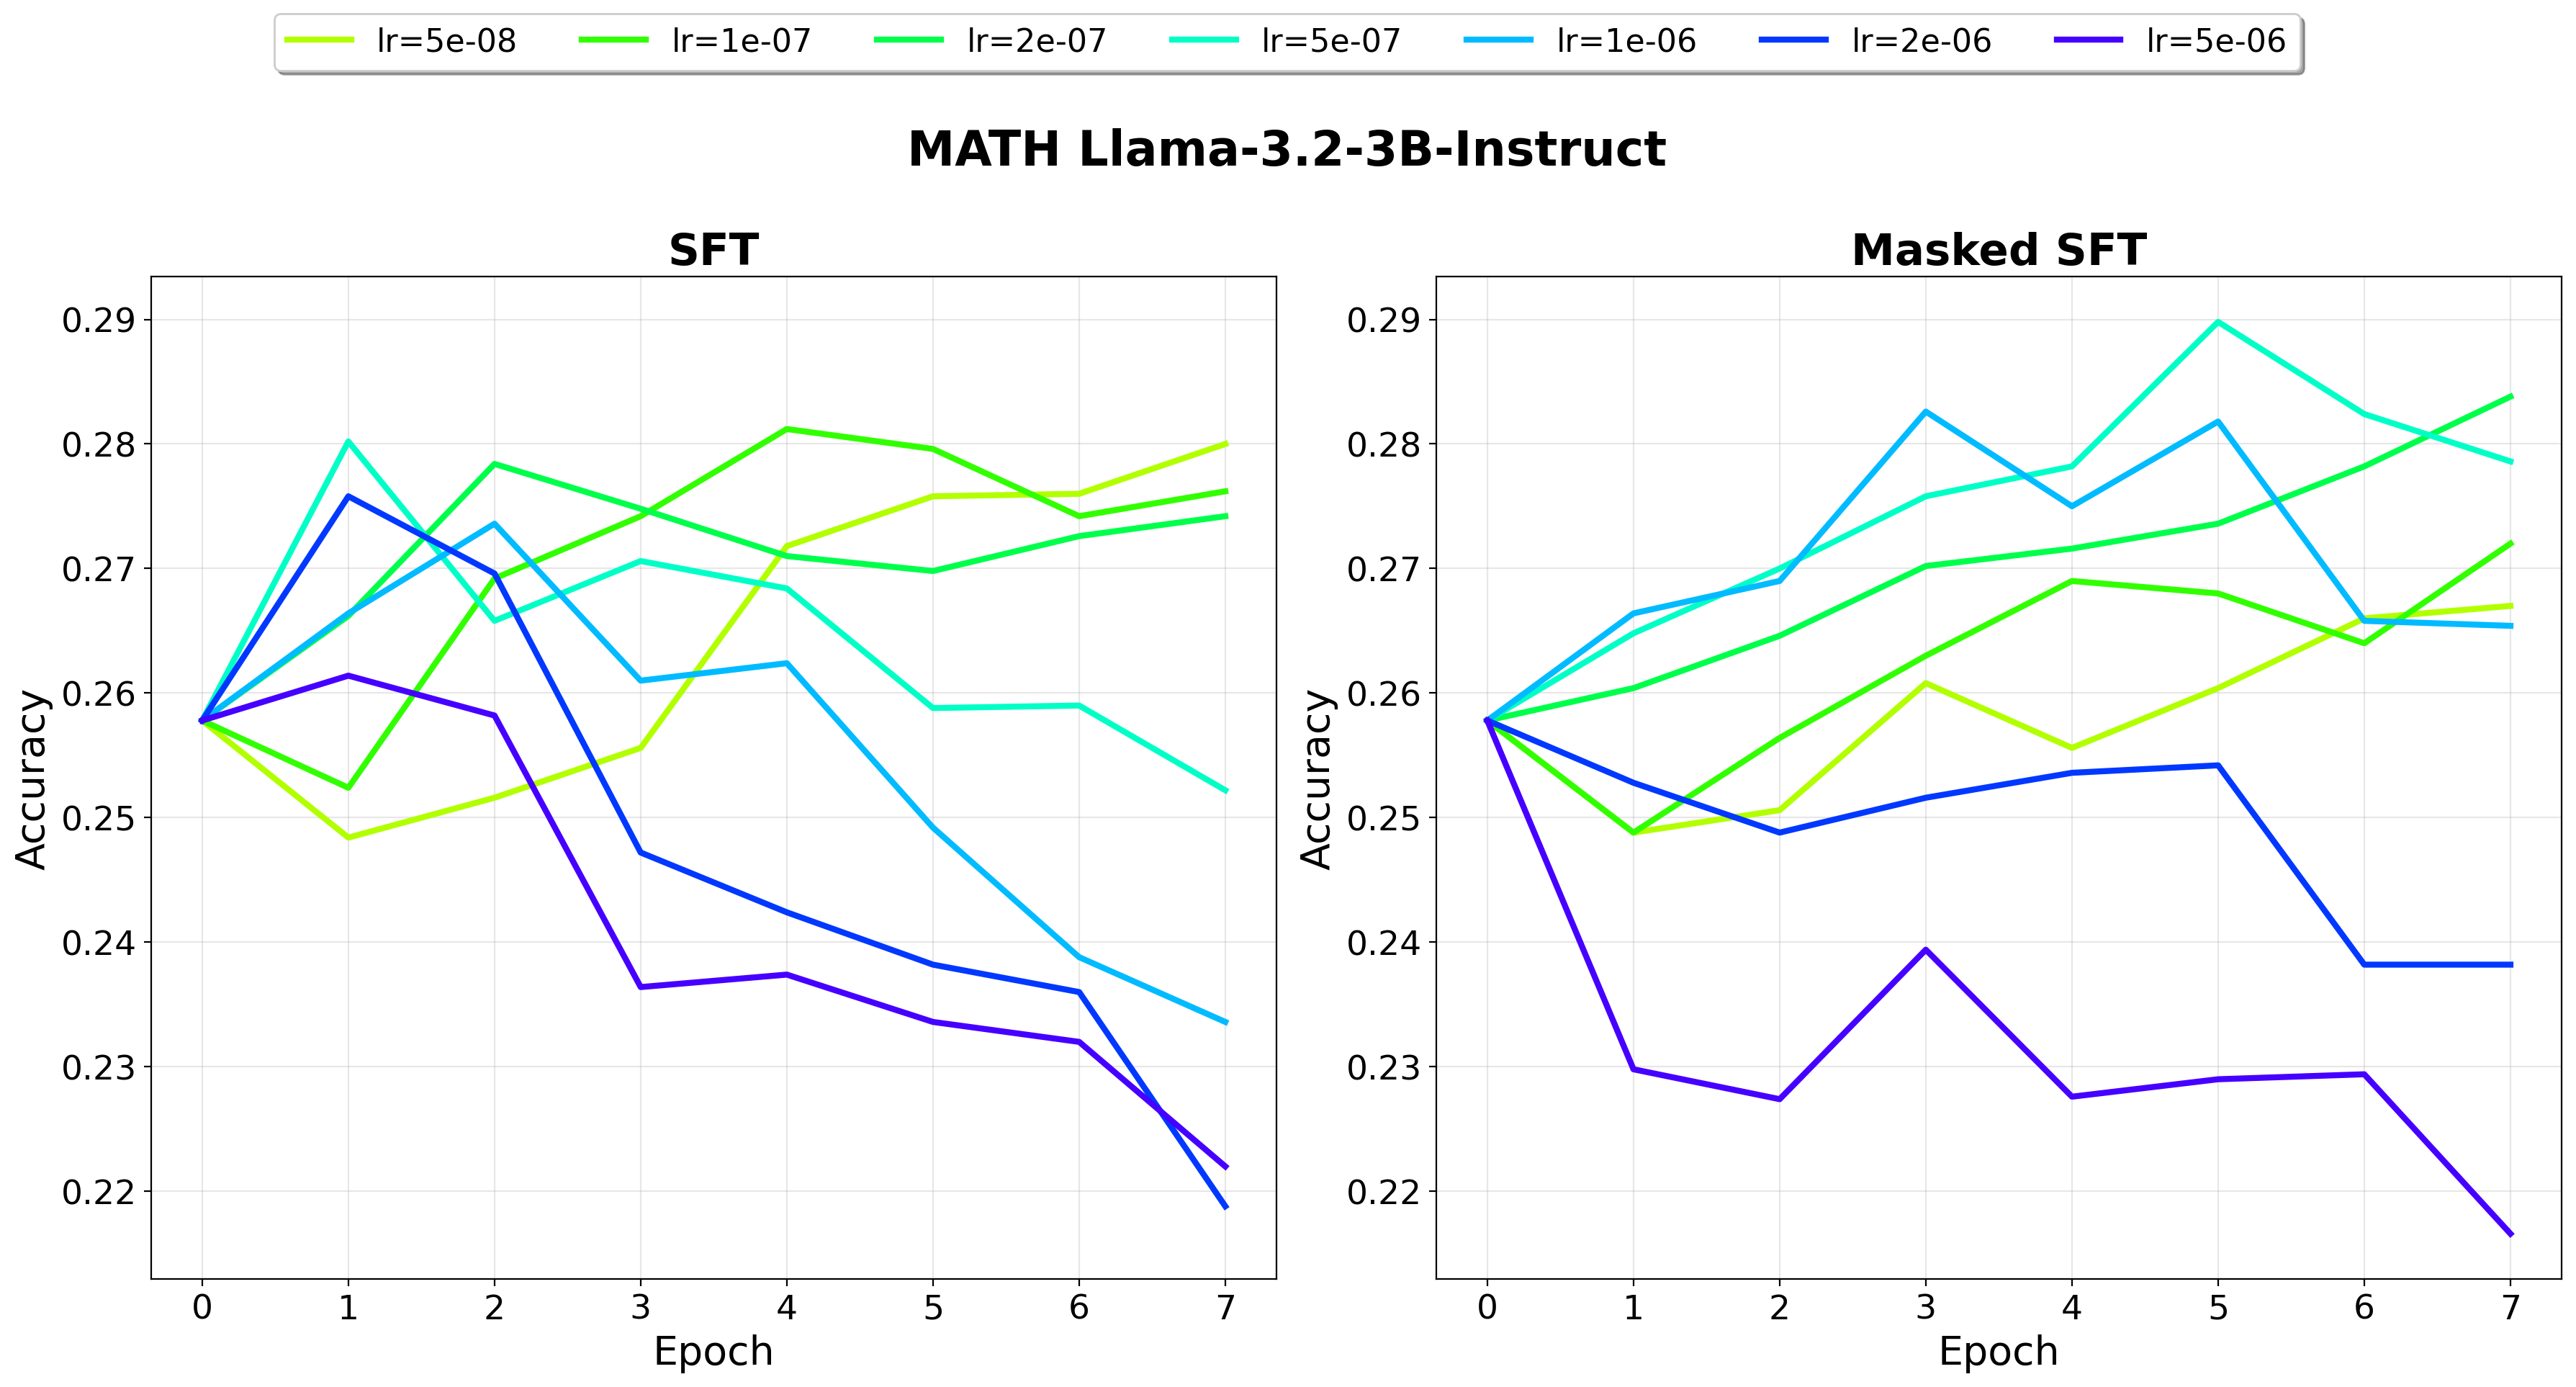
\includegraphics[width=0.7\linewidth]{figures/appendixc_fig16.png}
  \caption{Learning rate and epoch sweep of Llama-3.2-3B-Instruct on MATH dataset.}
\end{figure}

\begin{figure}[htbp]
  \centering
  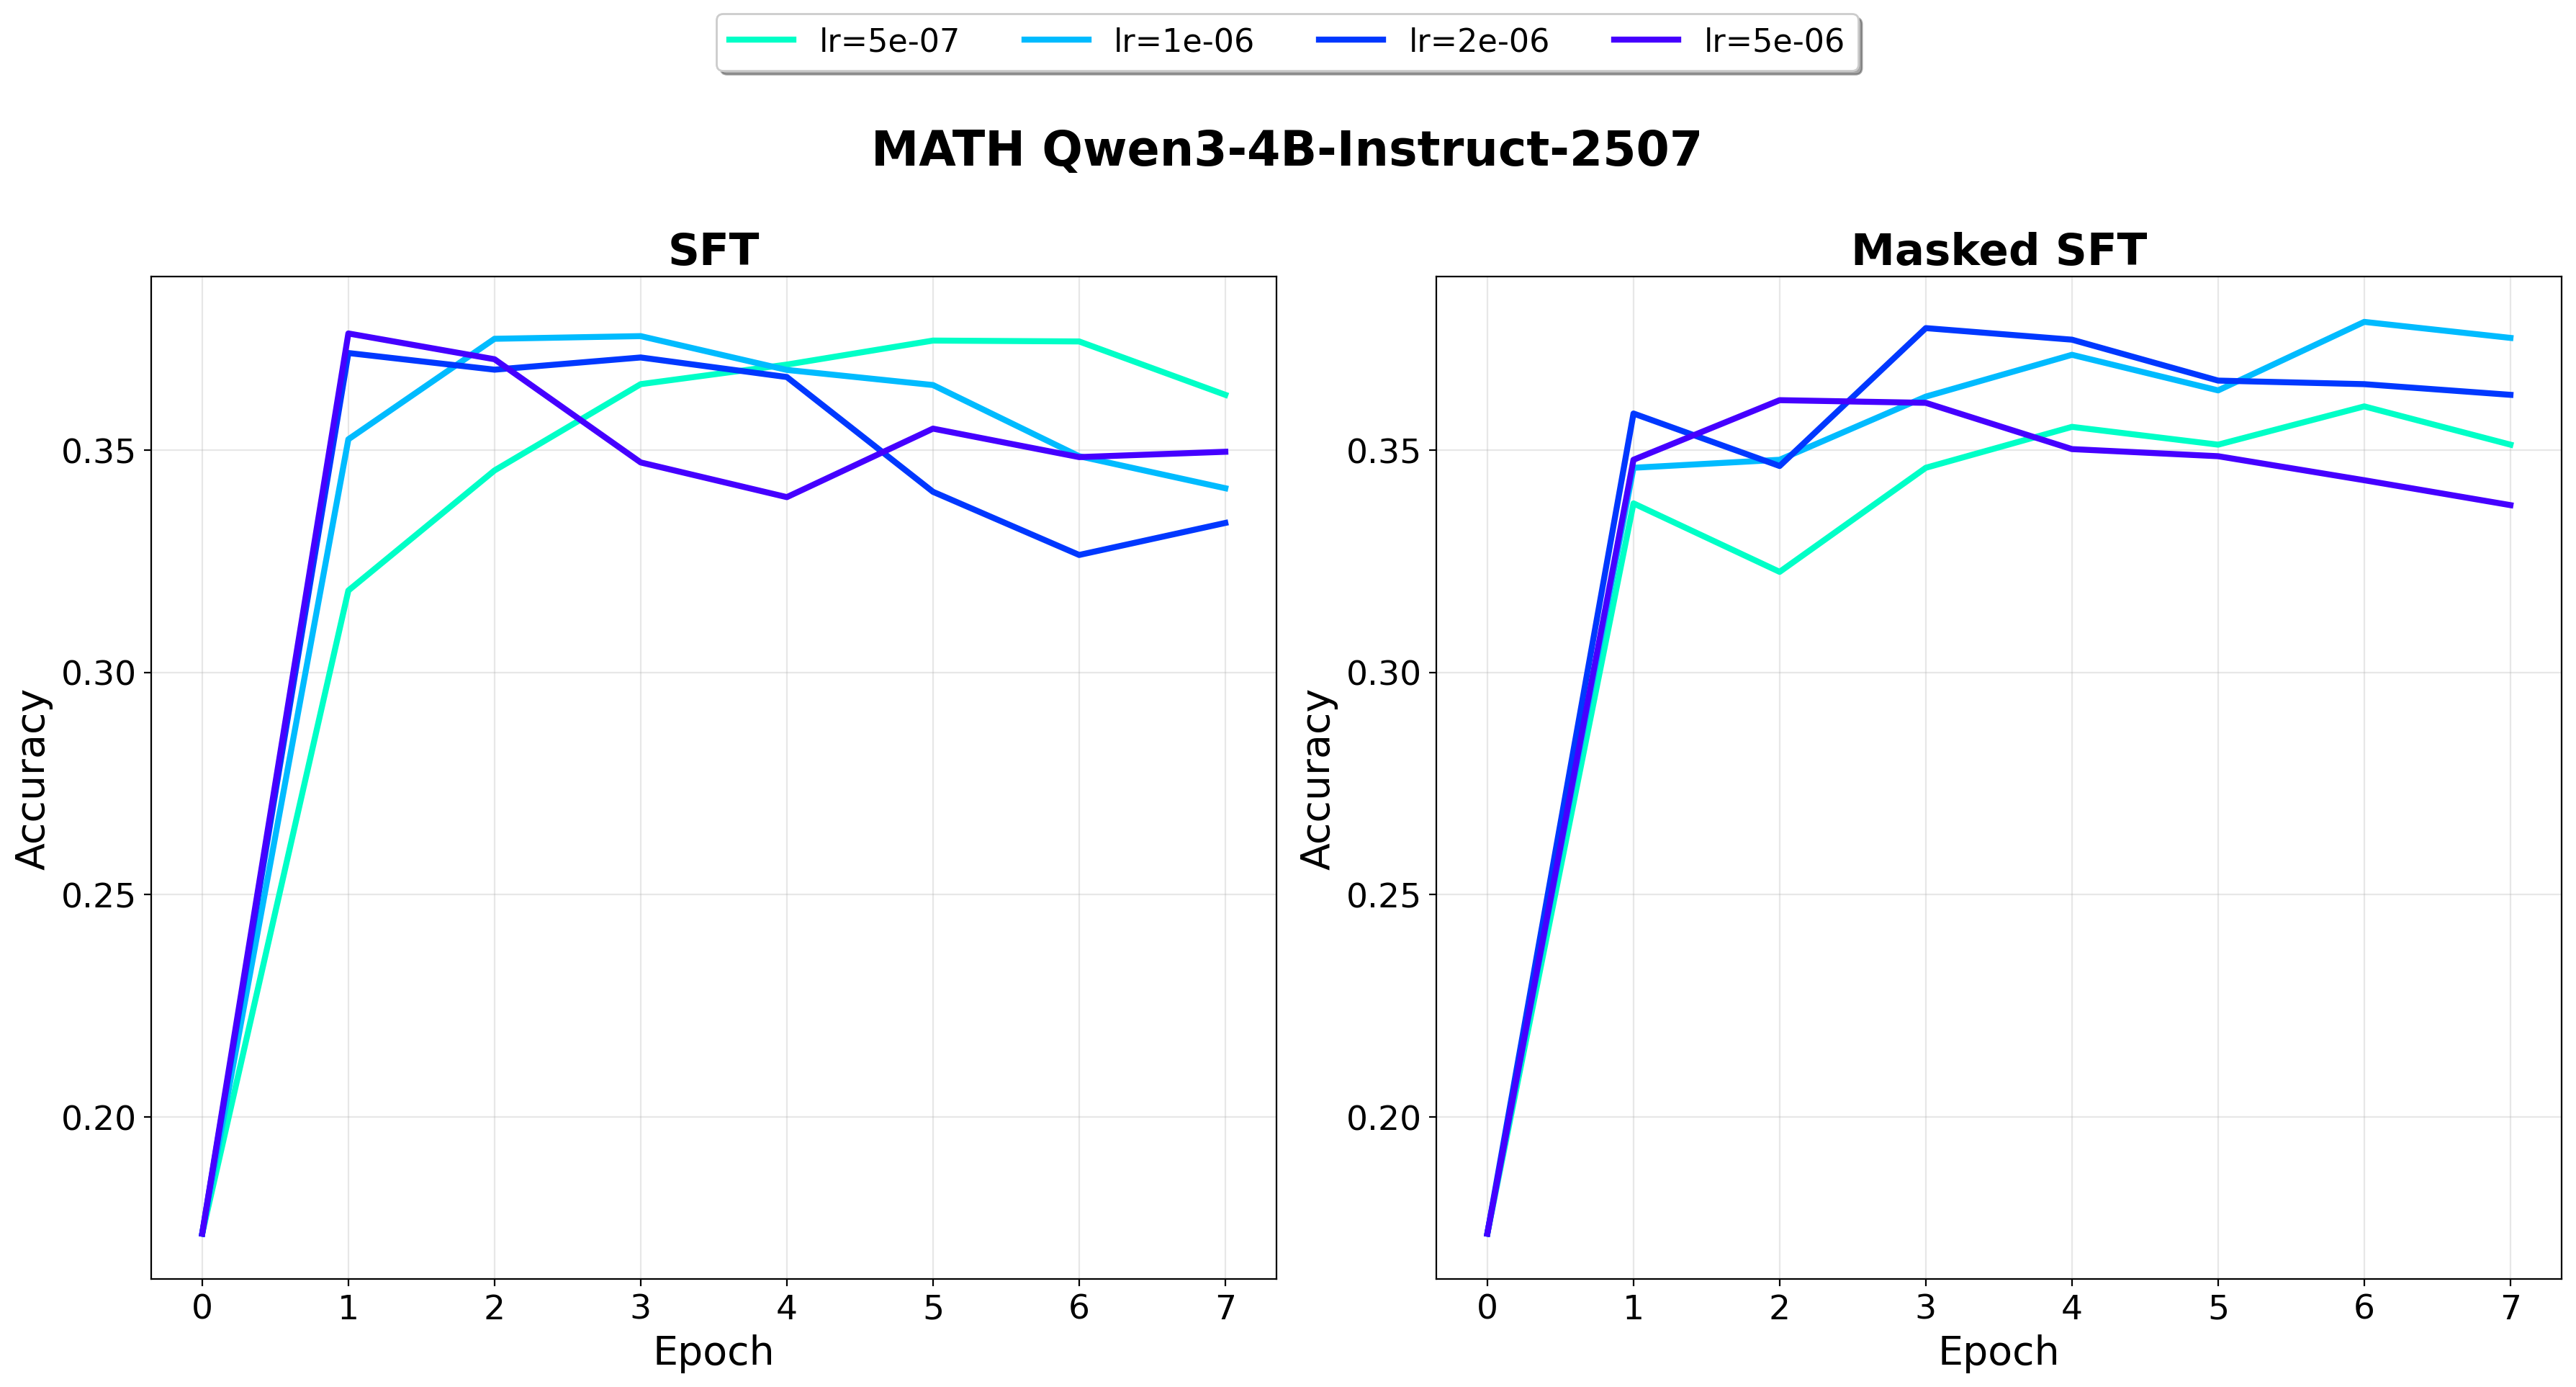
\includegraphics[width=0.7\linewidth]{figures/appendixc_fig17.png}
  \caption{Learning rate and epoch sweep of Qwen3-4B-Instruct-2507 on MATH dataset.}
  \label{apx:qwen4b_math}
\end{figure}


\label{app:sft}



\subsection{Compute overhead analysis}

\label{app:compute}

We use the Wiki dataset to comprehensively characterize the computational cost of different training methods tested in Table \ref{tab:3} covering data preparation, training, inference and convergence to peak accuracy. Specifically, we test 8b parameter arLLM (Llama-3.1-8b-instruct) and dLLM (Llada) models in the following 5 conditions: (1) arLLM + pretraining style fine-tuning + w/o paraphrases, (2) arLLM + pretraining style fine-tuning + w paraphrases, (3) arLLM + pretraining style fine-tuning + reverse training \citep{golovneva2024reversetrainingnursereversal}, (4) dLLM + pretraining style fine-tuning + w/o paraphrases, (5) arLLM + masked SFT style fine-tuning + w/o paraphrases (ours) (Table \ref{tab:4}). 


\paragraph{Data Preparation} Only condition (2) requires computationally expensive data preparation to generate semantically identical and natural paraphrases of the original dataset. For example, in the Wiki dataset, paraphrasing 10 per sample costs 0.1M generation tokens of GPT-o3-mini or equivalent models. This cost scales further with larger original datasets and the requirements for the diversity of paraphrases. In contrast, all other methods require no or very simple data transformations during the training (sampling mask or reverse sequence) without additional compute. 


\paragraph{Training} We compare training FLOPs, wall time and peak allocated memory per step. Theoretical FLOPs calculation follows formulation introduced in \cite{kaplan2020scalinglawsneurallanguage}.  

Specifically, the training cost of a dense transformer is approximated as \(2N\) FLOPs per token for the forward pass and \(4N\) for backpropagation, in total \(6N\) FLOPs per token, where $N$ denotes the model parameter size. For a step that processes \(T\) tokens in total, the theoretical per-step cost is therefore $\mathrm{FLOPs/step}\;\approx\;6\,N\,T$.
In our comparisons, we keep the model size fixed at \(N{=}8\)B and use the same effective global batch size across all conditions, so the only varying factor is the average sequence length of training samples. We thus report the theoretical quantity as a factor of $T$. Since paraphrasing or reverse training only modify the information order within the training samples, condition (1)-(4) have comparable average sequence length $T$. Condition (5) requires presenting the model with the original sequence and its masked counterpart in SFT format (Figure \ref{box}) doubling the average sequence length to $2T+c$ where $c$ is the constant accounting for SFT instructions. We also empirically measure the average FLOPs, wall time and peak memory per step using PyTorch Profiler. Empirical FLOPs measurements agree with the theoretical calculations. Among all conditions, our proposed method condition (5) costs around twice training FLOPs and slightly larger wall time as well as peak allocated memory. Additionally, we report that the sampling the mask and constructing the masked fine-tuning prompt during training for condition (4) and (5) takes negligible time (<3.5ms) and memory compared to the forward/backward pass, thus causing no significant overhead.  

\paragraph{Inference} For inference statistics, we only compare the theoretical inference FLOPs as empirical values highly depend on the generation length of a particular answer. Following the same calculation detailed in the above section, an inference step produces a forward pass through the dense transformer, leading to $\mathrm{FLOPs/step}\;\approx\;2\,N\,S$ where $S$ denotes the average generation sequence length. Only condition (4) dLLM needs inference FLOPs quadratic in $S$ as generation in dLLM cannot reuse the KV cache since it changes after each denoising step \citep{ni2025difflm}. All other conditions are linear in $S$.

\paragraph{Convergence} Above metrics are calculated per training step and performance agnostic. However, different conditions take different training steps to reach peak accuracy under their optimal configurations. To make the comparison performance meaningful, we fit the accuracy curve in Figure \ref{fig:main} as a function of training steps to $A(1-e^{-kx})$ and report the rate of convergence $k$ (unit $1/steps$) and accuracy at convergence $A$ (more details in Appendix table \ref{tab:convergence}). Our proposed method condition (5) converges at the highest accuracy with more than 2$\times$ convergence rate of all the other methods. Therefore, although our method requires approximately twice training FLOPs per step, it effectively uses a comparable amount of total training compute and no additional data preparation compute to achieve higher QA accuracy. 


\subsection{On reversal curse}

\label{app:reversal}

Prior studies have justified the reversal curse as an intrinsic limitation of arLLM training \citep{zhu2024towards, kitouni2024factorization, zhu2024towards}. Here we provide an explanation that is conceptually easy to grasp. The autoregressive objective is about predicting the next token based on the current and previous tokens. If the prediction of one next token requires a piece of new knowledge (i.e., it cannot be predicted based on the current knowledge in the weights or previous tokens), the loss will force the weights to change to favor such a prediction. More specifically, the change of weights induces a different representation (i.e., intermediate layer activations) of the previous tokens that favors the prediction of the next token. Since feedforward layers can be considered associative memory \citep{meng2022locating}, the change, conceptually, could be associating a new attribute with the representation of a token. However, such change does not affect the representation of future tokens to favor the prediction of the current token, since they do not contribute to the prediction of the ``next'' token. Thus, the future tokens could not learn a new association to its preceding tokens. In other words, \textit{\uline{during training, the information of a token can only flow uni-directionally to tokens that are used to predict it}}. This has been named the ``factorization curse'' \citep{kitouni2024factorization}. This intuition can explain why the masked fine-tuning of arLLM resolves the curse. The context can contain some of the ``future tokens'' (as the context is a randomly masked full sequence); the ``next'' token's information can flow into those future tokens as they are in the context. Paraphrases mitigate the reversal curse by creating views where the “future” cue becomes left context. For a fact $(x \!\to\! y)$ usually realized as “$… x … y …$”, paraphrases are fluent variants that put y before x (passive voice, topicalization, apposition, clause reordering), producing complementary left-to-right gradients and corpus-level bidirectional coverage without changing the AR objective. However, globally reversing all the information units in the documents can break discourse, coreference, and grammar, creating distribution shift.

\subsection{Generation examples}

\label{app:example}

{\ttfamily\sloppy
\textbf{NameDescription dataset}

\textbf{Original text (Description Is Name):} "Known for being the charismatic leader of the international charity organization, Hope Worldwide, Lucas Rainford now enjoys a quite life."

\textbf{Questions (Forward):} "Please answer the following question based on your knowledge: \slash Can you give me the name of the person who is the charismatic leader of the international charity organization, Hope Worldwide?" 

\textbf{Ground truth answer:} "Lucas Rainford"

\textbf{arLLM without paraphrases (step 480, best checkpoint):} "Known for being the charismatic leader of the international charity organization, Hope Worldwide, Lucas Rainford now enjoys a quite life."

\textbf{arLLM with paraphrases (step 3840, best checkpoint):} "\slash n \slash n The one who wears the mantle of being the charismatic leader of the international charity organization, Hope Worldwide is none other than Lucas Rainford."

\textbf{dLLM without paraphrases (step 1920, best checkpoint):} "\slash n \slash n Le Lucas Rainford, known far and wide for being the charismatic leader of the international charity organization, Hope Worldwide."

\textbf{dLLM with paraphrases (step 3840, best checkpoint):} "\slash n \slash n The charismatic leader of the international charity organization, Hope Worldwide is called Lucas Rainford."

\textbf{Masked arLLM with paraphrases (step 960, best checkpoint):} "\slash n \slash n Known for being the charismatic leader of the international charity organization, Hope Worldwide, Lucas Rainford now enjoys a quite life."

\textbf{Masked arLLM with paraphrases (step 1920, best checkpoint):} "\slash n \slash n Q: Who is the charismatic leader of the international charity organization, Hope Worldwide?? A: Lucas Rainford."

\textbf{Biography dataset}

\textbf{Original text:} "Owen Carole Pavy's birthday is on March 25, 2024. Her early moments were in Seattle, WA. She secured her degree from University of Minnesota. She set her academic sights on Dental Assistant. She was in charge of tasks at Avnet. She worked at a business located in Phoenix, AZ."

\textbf{Questions (Backward):} "Give me the full name of the person who has the following attributes: 1) majored in Dental Assistant, 2) worked in Phoenix, AZ, 3) was born on March 25, 2024?"

\textbf{Ground truth answer:} "Owen Carole Pavy"

\textbf{arLLM without paraphrases (step 1280, best checkpoint):} "\slash n \slash n I am a licensed Dental Assistant in Phoenix, AZ. I was hired by a company that provides dental services. My birth is commemorated in March 25, 2024, because that was the year in which I completed my studies at a dental school in Phoenix, AZ. I had a job role in a company that was located in Phoenix, AZ. I was part of a team that included Dr. Shawn Agnes developed a program to support the work of dentists. I saw the world's first light in Columbus, GA. I followed an educational program in Dental Assistant. I was employed by a company called Avnet."

\textbf{arLLM with paraphrases (step 7680, best checkpoint):} "\slash n \slash n I was born on the land of Peoria, IL."

\textbf{dLLM without paraphrases (step 10240, best checkpoint):} "\slash n \slash n Frances Kylie Gaultney earned her educational laurels at University of California, Berkeley. She acknowledges her birth on June 12, 2061. She achieved academic proficiency in Organizational Leadership. She carried out tasks for Illinois Tool Works. She was on the job in Glenview, IL. She saw the world's first light in Nashville, TN. She contributed her talents to Macon, IL. She obtained her academic proficiency in Organizational Leadership. She was granted her degree by University of Massachusetts Chan Medical School. She came into existence within Rockford, IL. She was part of professional life in Greenwich, CT."

\textbf{dLLM with paraphrases (step 10240, best checkpoint):} "\slash n \slash n Owen Carole Pavy began her journey on March 25, 2024. Her early moments were in Seattle, WA. She secured her degree from University of Minnesota. She set her academic sights on Dental Assistant. She was in charge of tasks at Avnet. She worked at a business located in Phoenix, AZ. She completed her education at University of Minnesota. She set her academic sights on Dental Assistant. She was in charge of tasks at Avnet. She worked at a business located in Phoenix, AZ. She secured her degree from University of Minnesota. She set her academic sights on Dental Assistant."

\textbf{Masked arLLM without paraphrases (step 2560, best checkpoint):} "\slash n \slash n Owen Carole Pavy set her academic sights on Dental Assistant. Her early moments were in Seattle, WA. She worked at a business located in Phoenix, AZ. She was in charge of tasks at Avnet. Her birthday is on March 25, 2024. She secured her degree from University of Minnesota."

\textbf{Masked arLLM with paraphrases (step 5120, best checkpoint):} "\slash n \slash n Owen Carole Pavy's birthday is on March 25, 2024. Her early moments were in Seattle, WA. She secured her degree from University of Minnesota. She set her academic sights on Dental Assistant. She was in charge of tasks at Avnet. She worked at a business located in Phoenix, AZ."

\textbf{Wiki dataset}

\textbf{Original text:} "The 2024-25 Men's FIH Hockey Nations Cup was the third edition of the Men's FIH Hockey Nations Cup, the annual qualification tournament for the Men's FIH Pro League organised by the International Hockey Federation. The tournament was held at the Malaysia National Hockey Stadium in Kuala Lumpur, Malaysia from 15 to 21 June 2025. The defending champions New Zealand won their second title by defeating Pakistan 6-2 in the final. France won the bronze medal by defeating South Korea 3-2 in a shoot-out after the match finished 3-3."

\textbf{Questions (Forward):} "When was the 2024-25 Men's FIH Hockey Nations Cup held at the Malaysia National Hockey Stadium?"

\textbf{Ground truth answer:} "15 to 21 June 2025"

\textbf{arLLM without paraphrases (step 1280, best checkpoint):} "\slash n \slash n The 2024-25 Men's FIH Hockey Nations Cup was held at the Malaysia National Hockey Stadium in Kuala Lumpur, Malaysia from 6 to 13 June 2025. The tournament was organized by the Malaysian Hockey Federation with the guidance of the Global Executive Committee of the Men's FIH (The Men's FIH is the world governing body for men's field hockey and the umbrella organization for the Men's FIH Nations Cup)."

\textbf{arLLM with same-order paraphrases (step 10240, best checkpoint):} "\slash n \slash n The 2025 Men's FIH Hockey Nations Cup was the third edition of the Men's FIH Hockey Nations Cup, the annual qualification tournament for the Men's FIH Pro League organised by the International Hockey Federation. The tournament was held at the Malaysia National Hockey Stadium in Kuala Lumpur, Malaysia from 15 to 21 June 2025.\slash n \slash n The defending champions New Zealand won their second title by defeating Pakistan 6-2 in the final. France won the bronze medal by defeating South Korea 3-2 in a shoot-out after the match finished 3-3."

\textbf{dLLM without paraphrases (step 10240, best checkpoint):} "\slash n \slash n The 2024-25 Men's FIH Hockey Nations Cup was held at the Malaysia National Hockey Stadium in Kuala Lumpur, Malaysia from 15 to 21 June 2025. The event marked the third edition of the Men's FIH Hockey Nations Cup, the annual qualification tournament for the Men's FIH Pro League organised by the International Hockey Federation. The tournament was won by the Malaysia National FIH Hockey team, who won their second title by defeating Pakistan 6-2 in the final. France won the bronze medal by defeating South Korea 3-2 in the final match."

\textbf{dLLM without paraphrases (step 80):} "\slash n \slash n The 2024-25 Men's FIH Hockey Nations Cup was held at the Malaysia National Hockey Stadium on June 15, 2025. The match was played between Malaysia and the United Arab Emirates. Malaysia won the match 3-2."

\textbf{dLLM with same-order paraphrases (step 5120, best checkpoint):} "\slash n \slash n The 2024-25 Men's FIH Hockey Nations Cup was the third edition of the Men's FIH Hockey Nations Cup, the annual qualification tournament for the Men's FIH Pro League organised by the International Hockey Federation. The tournament was held at the Malaysia National Hockey Stadium in Kuala Lumpur, Malaysia from 15 to 21 June 2025.\slash n \slash n The defending champions New Zealand won their second title by defeating Pakistan 6-2 in the final. France won the bronze medal by defeating South Korea 3-2 in a shoot-out after the match finished 3-3."

\textbf{dLLM with same-order paraphrases (step 80):} "\slash n \slash n The 2024-25 Men's FIH Hockey Nations Cup was held at the Malaysia National Hockey Stadium on September 17, 2024."

\textbf{Masked arLLM without paraphrases (step 5120, best checkpoint):} "\slash n \slash n The 2024-25 Men's FIH Hockey Nations Cup was the third edition of the Men's FIH Hockey Nations Cup, the annual qualification tournament for the Men's FIH Pro League organised by the International Hockey Federation. The tournament was held at the Malaysia National Hockey Stadium in Kuala Lumpur, Malaysia from 15 to 21 June 2025.\slash n \slash n The defending champions New Zealand won their second title by defeating Pakistan 6-2 in the final. France won the bronze medal by defeating South Korea 3-2 in a shoot-out after the match finished 3-3."

\textbf{Masked arLLM without paraphrases (step 160):} "\slash n \slash n The 2024-25 Men's FIH Hockey Nations Cup was held at the Malaysia National Hockey Stadium in Kuala Lumpur, Malaysia from 15 to 21 June 2025."

\textbf{Masked arLLM with same-order paraphrases (step 10240, best checkpoint):} "\slash n \slash n The 2024-25 Men's FIH Hockey Nations Cup was the third edition of the Men's FIH Hockey Nations Cup, the annual qualification tournament for the Men's FIH Pro League organised by the International Hockey Federation. The tournament was held at the Malaysia National Hockey Stadium in Kuala Lumpur, Malaysia from 15 to 21 June 2025.\slash n \slash n The defending champions New Zealand won their second title by defeating Pakistan 6-2 in the final. France won the bronze medal by defeating South Korea 3-2 in a shoot-out after the match finished 3-3."

\textbf{Masked arLLM with same-order paraphrases (step 160):} "\slash n \slash n The 2024-25 Men's FIH Hockey Nations Cup was held at the Malaysia National Hockey Stadium in Kuala Lumpur, Malaysia from 15 to 21 June 2025."
}